\documentclass[a4paper,pdftex,12pt]{book}
\usepackage[pdftex]{graphicx}
\usepackage[portuguese]{babel}
%\usepackage[activeacute,spanish, portuguese]{babel}
% \usepackage[T1]{fontenc}
% \usepackage[protrusion=true,expansion=true]{microtype}
 \usepackage{enumitem}
% \usepackage{libertine}
% \usepackage[latin1]{inputenc}
 \usepackage{geometry}
% % \geometry{verbose,dvips,,tmargin=.65in,bmargin=.9in, left=0.80in, right=0.65in}
 \geometry{verbose,dvips,tmargin=2cm,bmargin=2cm, left=2.5cm, right=3.5cm}
% \usepackage{lettrine}
 \usepackage[raggedright]{titlesec}
 \usepackage{booktabs}
 \usepackage[all]{nowidow}
% %\usepackage{soul}
 \usepackage{bookmark}

% \newcommand{\degree}{\ensuremath{^\circ}}
% Substituído por \textdegree 

% %\renewcommand{\textbf}[1]{\ul{#1}}

\setcounter{secnumdepth}{0} 
\setcounter{tocdepth}{2}

\titleformat{\section}
  {\raggedright\normalfont\scshape}{\thesection}{1em}{}
	
\titleformat{\subsection}
  {\raggedright\normalfont\slshape}{\thesection}{1em}{}	
	
\brokenpenalty=10000\relax

% \setlist[itemize]{leftmargin=*, noitemsep}

\makeatletter
\def\@makechapterhead#1{%
  \vspace*{20\p@}%
  {\parindent \z@ \raggedright
    \Large
    \ifnum \c@secnumdepth >\m@ne
        \textsc{\Large#1}
        \par\nobreak    
    \fi
    \interlinepenalty\@M
    \vskip 110\p@
  }}
  
  \def\notesname{}%


\def\@makeschapterhead#1{%
  \vspace*{20\p@}%
  {\parindent \z@ \raggedright
    \Large
    \ifnum \c@secnumdepth >\m@ne
        \textsc{\Large#1}
        \par\nobreak    
    \fi
    \interlinepenalty\@M
    \vskip 110\p@
  }}
  
  \def\notesname{}%

\makeatletter

 \usepackage{fancyhdr}
 \fancyhead[LE,RO]{}
 \fancyhead[CE,CO]{}
 \fancyhead[RE,LO]{}
 \fancyfoot[LO,RE]{}
 \fancyfoot[CE,CO]{}
 \fancyfoot[LE,RO]{\thepage}

 \usepackage{hyperref}

\begin{document}

 \renewcommand{\headrulewidth}{0pt}

 \normalsize

  % \newpage
  % \thispagestyle{empty}
  % \mbox{}

  % \newpage
  % \thispagestyle{empty}
  % \mbox{}

\begin{frontmatter}
\pagestyle{empty}

\vspace*{3cm}
\begin{center}
  
  \Large{\textit{Introdução aos SIG}  } \\
  \Large{\textit{Introducción a los SIG}}
\end{center}
\cleardoublepage


\makeatletter
\newlength\drop
\newcommand*{\titleGM}{%
  \thispagestyle{empty}
  \begingroup% Gentle Madness
    \drop = 0.05\textheight
    \vspace*{\baselineskip}
    \vfill
     \hbox{%
       \hspace*{0.1\textwidth}%
       \rule{1pt}{\dimexpr\textheight-28pt\relax}%
       \hspace*{0.05\textwidth}% 
       \parbox[b]{0.75\textwidth}{%
         \vbox{%
             \vspace{\drop}
             {\Large\textsc{Víctor Olaya}\par}\vskip3.5\baselineskip
             {\Huge\raggedright{\textsc{Introducción}\\\textsc{a los SIG}}\par}
             \vspace{0.62\textheight}
         }% end of vbox
       }% end of parbox
    }% end of hbox

    \vfill
    \null
  \endgroup}
\makeatother
\titleGM

\null
\vfill
\scriptsize
\noindent
Introducción a los SIG.\\ 
Copyright \copyright 2016 Víctor Olaya.\\
Imagen de cubierta: The Art Journal; \textit{The Industry of All Nations Illustrated Catalogue} (London, England: Bradbury and Evans, 1851)

\cleardoublepage

 \normalsize

  \chapter*{Prefácio}

Por anos temos utilizado o livro do Victor em nosso curso de Especialização em Geoprocessamento aqui na Universidade Federal de São Carlos. Entretanto, muitos de nossos alunos não o usam por terem dificuldade de ler tanto a versão em Inglês quanto a versão em Espanhol.

Assim, decidi iniciar uma versão traduzida para o portugues, com o objetivo de disseminar este excelente livro entre meus alunos de graduação e de pós-graduação, bem como para toda a comunidade de falantes da lingua portuguesa.

A tradução será feita inicialmente com apoio de ferramentas baseadas em Inteligência Artificial, seguida por minha revisão. No decorrer do processo deixarei explícito o estado da tradução (IA ou revisado).

Como a \textsc{Gretchen Peterson} Co-autora do \textit{QGIS Map Design} diz em seu prefácio em inglês, Victor generozamente disponibiliza este livro para todos os usuários, de maneira gratuíta. 



\begin{flushright}
    \textsc{Edson Augusto Melanda}\\
    Diretor do NGeo-UFSCar \\
    Universidade Federal de São Carlos\\
    Brasil
    \end{flushright}
 \chapter*{Prólogo}

Hace ahora más de cinco anos que se publicó la primera versión de \textit{Sistemas de Información Geográfica}, un libro libre sobre fundamentos de SIG en español, y apenas unos meses desde que apareció la segunda. El libro ha tenido una acogida excelente, y mi intención es seguir manteniéndolo actualizado en la medida que sea posible, reflejando los avances que, a buen seguro, van a producirse en el campo de los SIG.

Existe, no obstante, un obstáculo importante para que el libro alcance a todos los públicos: su tamaño. Por su completitud, y por la complejidad propia de la disciplina, el libro es un volumen de más de 800 páginas cargadas de detalle. La segunda versión se presenta en un único tomo, frente a los dos en que consistía la primera, pero aún así sigue quedando como una obra de consulta demasiado extensa para leerse de principio a fin. Para el lector que comienza a introducirse en el ambito de los SIG y no busca especializarse, resulta un volumen intimidante y es, no hay duda, difícil de abordar.

Este libro intenta ser una alternativa a la obra completa, de tal forma que resulte más accesible para quienes desean tener una perspectiva global de la disciplina de los SIG, sin entrar en detalles demasiado específicos. Es, basicamente, una versión resumida de aquel, pensada con la idea de usarse no como libro de consulta, sino como libro de lectura. Además de ser más breve, se presenta en un formato más adecuado para esta clase de propósito, con algunas modificaciones en su enfoque y con menos contenido gráfico.

He respetado en líneas generales la estructura de los capítulos, de modo que es fácil para el lector que desee profundizar en uno de ellos encontrar este en el libro completo. Desde ese punto de vista, puede entenderse este libro como una especie de <<índice>> de su hermano mayor, un índice, no obstante, prolijo y con suficiente información como ofrecer al lector una visión detallada del mundo de los SIG.

Este es también, por supuesto, un libro libre, que espero que progrese de una forma dinámica gracias a la contribución de sus lectores. Si encuentras cualquier error o quieres colaborar en mejorar estas páginas, no dudes en escribirme a \\ \texttt{volayaf@gmail.com}.
  \chapter*{Foreword}\label{foreword}

I first met Victor when we were working at the same company. During that time I learned a few interesting things about him. Like how he works at such a rapid pace that if you blink you might find that he's written a new plugin for QGIS or even that he's written a book like this one. Aside from these great qualities, the thing I most remember about him is that he helped direct me to the last packet of hot chocolate in the office kitchen, after a day full of meetings when I needed it the most. It's helpful things like that which make a difference to people. And in this book you will find so many helpful things, akin to that hot chocolate but for Geographic Information Systems (GIS), organized in a thoughtful manner which will help you get through that sometimes-long GIS slog.


This book is an excellent reference text regarding the history and basics of GIS. It includes clear examples of concepts illustrating choices the geospatial professional must make in design and layout and how those choices affect a map product. The reader can literally see how decisions about line, color, shape, and other qualities will render a map that is the most useful and the most aesthetic. It also includes important information about the various ways in which GIS data is obtained, how it is stored, and a great overview of GIS software.

The book begins with the history of GIS and proceeds into sections that discuss and define such topics as spatial analysis, data visualization, web mapping and data sources, among many others. I envision the book being used as a teaching tool, both in a formal setting and for self-learners. Additionally, for more experienced geospatial professionals, this book can be used in the initial ideation phase of creating a map, reminding us of the elements we need to consider and prioritize to meet the objectives for a particular map or analysis. It is really a digital pocket guide to GIS.

Victor is generously making his book available to all, free, for users. Knowing the hours of work that go into any book, I appreciate his attitude of community and contribution to the field of GIS. Learning and continually revisiting the fundamentals is paramount for success in our field. So pour yourself a good cup of hot chocolate and get started.  



\begin{flushright}
\textsc{Gretchen Peterson}\\
Co-author of QGIS Map Design
\end{flushright}

\end{frontmatter} 
\pagestyle{empty}

\cleardoublepage
\vspace*{3cm}
\begin{center} 
{\Large\scshape Introdução aos SIG}

\end{center}

\begin{mainmatter}

  \tableofcontents

   
\chapter{O que é um SIG?}

\pagestyle{fancy}

A maior parte das informações que manipulamos em qualquer tipo de disciplina está georreferenciada. Ou seja, trata-se de informação à qual pode ser atribuída uma posição geográfica, e que, portanto, vem acompanhada de dados adicionais relativos à sua localização.

Um \textbf{Sistema de Informação Geográfica} (SIG) é uma ferramenta para trabalhar com informações georreferenciadas. Em particular, um SIG é um sistema que permite a realização das seguintes operações:

\begin{itemize}
	\item \textbf{Leitura, edição, armazenamento} e, em termos gerais, \textbf{gestão} de dados espaciais.
	\item \textbf{Análise} desses dados. Isso pode incluir desde consultas simples até a elaboração de modelos complexos, e pode ser realizado tanto sobre a \textbf{componente espacial} dos dados (a localização de cada valor ou elemento), quanto sobre a \textbf{componente temática} (o valor ou o elemento em si).
	\item Geração de \textbf{documentos} como mapas, relatórios, gráficos etc.
\end{itemize}

Um SIG representa um avanço em relação aos mapas clássicos. Enquanto um mapa é uma representação de um conjunto de dados espaciais — representação essa de enorme importância —, no ambiente de um SIG ele é apenas um dos elementos do sistema. O SIG inclui não só os dados e sua representação, mas também as operações que podem ser realizadas sobre eles, que fazem parte integrante desse sistema.

O SIG é uma ferramenta versátil e de amplo alcance, e atualmente a grande maioria das disciplinas se beneficia do seu uso de alguma forma. Uma das principais razões para isso é o \textbf{caráter integrador} dos SIG. Abaixo estão alguns dos contextos principais em que o SIG exerce tal função integradora:

\begin{itemize}
\item \textbf{SIG como integrador de informações}. Um ponto comum entre muitas disciplinas é o fato de que seus objetos de estudo estão associados a uma localização no espaço. Isso permite combiná-los e obter resultados por meio de uma análise conjunta. Nesse contexto, o SIG é o ambiente necessário para incorporar essa informação georreferenciada e trabalhar com ela.

\item \textbf{SIG como integrador de tecnologias}. Muitas das tecnologias que surgiram nos últimos anos (e certamente muitas das que ainda surgirão) estão focadas no aproveitamento da informação espacial, e estão conectadas, em maior ou menor grau, a um SIG para ampliar seu alcance e capacidades. Por sua posição central entre essas tecnologias, os SIG também atuam como elo entre elas, conectando-as e permitindo uma interação fluida por meio de suas funcionalidades.

\item \textbf{SIG como integrador de pessoas}. As funções básicas que um SIG deve cumprir abrangem uma ampla gama de atividades e atendem às necessidades de usuários que anteriormente não possuíam um ambiente de trabalho comum tão bem definido. Isso resulta em melhor coordenação entre esses usuários, pois é a própria ferramenta que define as características das relações estabelecidas, deixando de depender exclusivamente do contexto de aplicação.

\item \textbf{SIG como integrador de teorias e fundamentos}. Inicialmente, podemos entender um SIG como a união entre duas ciências: a geografia e a informática. Contudo, uma análise mais aprofundada revela que o SIG incorpora elementos de diversas outras áreas, como as relacionadas à tecnologia e ao tratamento da informação (informática, banco de dados, processamento digital de imagens), ciências que estudam a Terra sob uma perspectiva física (geologia, oceanografia, ecologia), ciências humanas e sociais (antropologia, geografia, sociologia), ciências do conhecimento e cognição (psicologia, epistemologia), além das disciplinas que tradicionalmente integram saberes de diferentes domínios — com destaque para a própria geografia.

O termo \textbf{geomática}, formado a partir das palavras \emph{geografia} e \emph{informática}, é frequentemente utilizado para se referir a esse conjunto de ciências relacionadas aos SIG.
\end{itemize}

Com base em tudo isso, entende-se que um SIG é um sistema que integra tecnologia da informação, pessoas e dados geográficos, cuja principal função é capturar, analisar, armazenar, editar e representar dados georreferenciados.

Sob outra perspectiva, um SIG pode ser considerado composto por cinco blocos fundamentais:

\begin{itemize}
 \item \textbf{Dados.} Os dados são essenciais para que os demais componentes do SIG façam sentido e possam cumprir seu papel no sistema. A informação geográfica — razão de ser dos SIG — está contida nos dados. Por isso, conhecer detalhadamente sua natureza, origem, qualidade, bem como sua gestão e armazenamento, é indispensável para compreender adequadamente o funcionamento dos SIG.

 \item \textbf{Análise.} A análise é uma das funcionalidades básicas dos SIG, e uma das principais razões que motivaram seu desenvolvimento. O computador é uma ferramenta com grande capacidade de processamento, e isso pode ser aplicado aos dados espaciais para gerar resultados dos mais diversos tipos.

 Em algum grau, todo SIG incorpora procedimentos que permitem obter resultados a partir da análise dos dados espaciais. As vantagens de incluir esses processos em uma única ferramenta — o SIG — vão desde a \textbf{automação de tarefas} até a criação de novos processos, cujos resultados não poderiam ser obtidos de outra forma.

 \item \textbf{Visualização.} Qualquer tipo de informação pode ser representada graficamente, o que facilita sua interpretação. No caso específico da informação geográfica, a visualização não é apenas uma forma adicional de trabalhar com os dados — é a principal, pois estamos habituados a isso por meio dos mapas.

 Diferentemente de um mapa, que é por natureza gráfico, um SIG lida com dados puramente numéricos. Para apresentar uma utilidade semelhante à de um mapa, o SIG deve incluir recursos para gerar representações visuais a partir desses dados.

 A visualização de dados geográficos segue os mesmos princípios utilizados na cartografia impressa, e esses princípios devem ser dominados pelo usuário do SIG, uma vez que ele será responsável pelo design cartográfico e pela preparação dos elementos visuais para trabalhar com as representações criadas.

 \item \textbf{Tecnologia.} Este componente inclui tanto o \emph{hardware} onde as aplicações SIG são executadas, quanto o \emph{software} SIG em si. Além da plataforma, o \emph{hardware} também abrange periféricos comuns no trabalho com SIG, como os utilizados para entrada de dados geográficos e produção cartográfica.

 \item \textbf{Fator organizacional.} Refere-se aos aspectos ligados à coordenação entre pessoas, dados e tecnologia, bem como à comunicação entre esses elementos. Com a crescente complexidade dos SIG, a gestão das interações entre seus componentes torna-se cada vez mais importante.
\end{itemize}

Ao longo deste livro, detalharemos cada um desses blocos nos capítulos correspondentes.

\pagestyle{empty}


  %  \chapter{História dos SIG}

\pagestyle{fancy}

O desenvolvimento dos SIG desde sua origem até os dias atuais é notável. A popularização das tecnologias e os esforços de desenvolvimento realizados por um amplo leque de ciências beneficiárias dos SIG contribuíram para redefinir a disciplina e incorporar elementos que, na época, eram impensáveis.

Podemos situar a origem dos SIG no início da década de \textbf{1960}, como resultado da convergência de dois fatores principais: a \textbf{necessidade crescente de informação geográfica} e sua gestão eficiente, e o \textbf{surgimento dos primeiros computadores}.

As bases para o futuro surgimento dos SIG encontram-se alguns anos antes dessa década, com o desenvolvimento de novos enfoques em cartografia, como a \textbf{geografia quantitativa}, que antecipavam necessidades futuras que a informatização traria.

A primeira experiência relevante que combina geografia e informática ocorre em 1959, quando Waldo Tobler define os princípios de um sistema chamado MIMO (map in--map out), com o objetivo de aplicar os computadores ao campo da cartografia. Nesse sistema, ele estabelece os princípios básicos para a criação, codificação, análise e representação de dados geográficos em um ambiente computacional.

O primeiro Sistema de Informação Geográfica formalmente desenvolvido surge no Canadá. Esse sistema, chamado CGIS (Canadian Geographical Information Systems), foi desenvolvido no início da década de 1960 por Roger Tomlinson, amplamente conhecido como o <<pai do SIG>>.

Em meados dos anos 60, os aplicativos SYMAP e GRID estabelecem, respectivamente, as bases dos dois principais enfoques para manipulação de informação geográfica: o enfoque \textbf{raster} e o enfoque \textbf{vetorial}. Ambos serão explicados em detalhes mais adiante neste livro. Os conceitos fundamentais para análise raster foram estabelecidos pouco depois por Dana Tomlin, ao desenvolver a chamada \textbf{álgebra de mapas}.

Durante os anos 1960, os SIG se desenvolvem a partir desses elementos iniciais e passam a ser incorporados à comunidade cartográfica, deixando de ser apenas uma ferramenta experimental.

A evolução dos SIG percorre, desde então, várias etapas, avançando rapidamente sob influência de diversos fatores externos. Essa evolução ocorre na própria disciplina dos SIG, nas tecnologias de apoio, nos dados e nas técnicas e formulações utilizadas.

\section{A evolução dos SIG como disciplina}

Inicialmente, os SIG eram apenas uma combinação de elementos da cartografia quantitativa aliados aos sistemas computacionais da época. Eram um campo dominado por cartógrafos e geógrafos que buscavam adaptar seus conhecimentos às tecnologias emergentes. Com o tempo, no entanto, os SIG passaram a incorporar um \textbf{grande número de outras disciplinas}, cujas contribuições e influências se tornaram tão relevantes quanto — ou até mais — que as da cartografia ou geografia.

Coincidindo com os primeiros estágios de desenvolvimento dos SIG, surge uma preocupação crescente com o meio ambiente, o que favorece o desenvolvimento das ciências relacionadas — a maioria das quais se tornariam usuárias diretas dos SIG. O SIG passa a ser gradualmente integrado às atividades de \textbf{gestão ambiental}, como apoio essencial à sua análise.

No início da década de 1970, já é evidente que os SIG são ferramentas promissoras, e surgem não apenas esforços para seu desenvolvimento e consolidação, mas também conferências, simpósios e a inclusão da temática em \emph{currículos} universitários. Nos anos 1980, consolidam-se revistas e fóruns especializados que levarão a disciplina a um público mais amplo.

No setor comercial, a indústria dos SIG também se consolida nos anos 70. A \textbf{ESRI} (Environmental Systems Research Institute), empresa pioneira e líder do setor até hoje, é fundada em 1969, e seus produtos são fundamentais na transformação dos SIG em ferramentas amplamente adotadas. O primeiro SIG de código aberto, \textbf{GRASS} (Geographic Resources Analysis Support System), surge em 1985.

O maior avanço na incorporação dos SIG a contextos não profissionais ocorre na primeira década do século XXI, com o surgimento de serviços de mapeamento como o \textbf{Google Maps}. A popularização dos \textbf{navegadores GPS}, que incorporam elementos de representação e análise típicos dos SIG, é outro exemplo da sua disseminação junto ao público geral.

\section{A evolução da tecnologia}

Três são os principais blocos de desenvolvimento tecnológico que mais influenciaram os Sistemas de Informação Geográfica:

\begin{itemize}
 \item \textbf{Saídas gráficas.} A evolução das capacidades gráficas — intensa desde o início e ainda em curso — foi acompanhada de perto pelos SIG, que passaram a incorporar progressivamente melhorias tanto na visualização em tela quanto na geração de mapas impressos.

 \item \textbf{Armazenamento e acesso aos dados.} O crescimento do volume de dados geográficos exigiu avanços em capacidade de armazenamento e velocidade de leitura, para garantir uma operação fluida dos sistemas.

 \item \textbf{Entrada de dados.} Nos primeiros anos dos SIG, os dados geográficos eram obtidos de documentos em papel, digitalizados manualmente e armazenados em cartões perfurados. Desde esses sistemas mecânicos até os equipamentos atuais — com \emph{scanners} de alta precisão e técnicas de digitalização automatizada — o processo de entrada de dados evoluiu radicalmente.
\end{itemize}

Além desses fatores, a evolução dos computadores impactou todos os elementos de \emph{software}. Passou-se dos grandes computadores aos computadores pessoais, e os programas — como os próprios SIG — também fizeram essa transição.

A partir do final dos anos 1980, a elaboração e análise de cartografia se torna possível em PCs de baixo custo, afastando-se das grandes máquinas e sistemas dedicados de alto custo.

A evolução das plataformas segue adiante. Atualmente, há uma tendência de levar os SIG para \textbf{plataformas móveis}, como celulares e tablets, especialmente úteis para coleta de dados em campo. A integração com tecnologias de posicionamento global, como o GPS, torna essa prática ainda mais eficaz.

O surgimento da Internet transformou toda a sociedade, incluindo o campo dos SIG. O primeiro uso relevante é registrado em 1993 com o \emph{Xerox PARC}, o primeiro \textbf{servidor de mapas}. Em 1994, é lançado o primeiro atlas digital online — o Atlas Nacional do Canadá. Mais recentemente, os conceitos da Web 2.0 são aplicados aos SIG, possibilitando o surgimento do \textbf{Web Mapping}.

\section{A evolução dos dados}

As primeiras bases de dados geográficas continham \textbf{mapas digitalizados} ou elementos vetoriais derivados desses. A partir daí, novas fontes de dados com estruturas mais adequadas ao processamento digital começaram a surgir, criando uma relação bidirecional entre SIG e dados.

Um marco importante é o lançamento dos primeiros \textbf{satélites de observação da Terra}. As técnicas de fotografia aérea, originalmente militares e iniciadas no século XIX com balões, passam a ser utilizadas em escala global com os satélites. Em 1980, é criada a SPOT, primeira empresa comercial a fornecer imagens de satélite para toda a superfície terrestre.

As \textbf{tecnologias de posicionamento e localização} também representam fontes primárias de dados. O sistema GPS torna-se totalmente operacional em 1981, e em 2000 sua precisão é ampliada para uso civil.

Como as aplicações, os tipos de dados geográficos digitais tornam-se mais populares e recebem maior atenção. Em 1976, o USGS (Serviço Geológico dos EUA) publica os primeiros \textbf{Modelos Digitais de Elevação} (MDE). Em 2000, são divulgados os dados da \emph{Shuttle Radar Topographic Mission} (SRTM), cobrindo 80\% da superfície terrestre com resolução de aproximadamente 30 metros.

O surgimento de novas tecnologias, como o \textbf{LiDAR}, possibilita níveis de precisão antes inatingíveis e abre novas possibilidades de análise.

A evolução dos dados não é apenas técnica, mas também \textbf{social e organizacional}. Passa-se a entender a importância de estratégias adequadas para a gestão de dados espaciais, surgindo as chamadas \textbf{Infraestruturas de Dados Espaciais} (IDE). O maior exemplo é a NSDI, dos EUA (1994). Na Europa, destaca-se a diretiva INSPIRE, de 2007.

Muitos desses avanços seguem as diretrizes do \emph{Open GIS Consortium} (OGC), fundado em 1994 para \textbf{padronizar} o uso e disseminação de dados geográficos.

\section{A evolução das técnicas e formulações}

Após os primeiros SIG serem implementados, surgem novas técnicas e abordagens que ampliam as possibilidades de análise.

Um dos primeiros antecedentes da análise espacial ocorre em 1854, quando John Snow utiliza mapas de pontos para localizar a origem de um surto de cólera na Inglaterra — um exemplo clássico de cartografia analítica.

Em seu livro \emph{Design with Nature} (1969), Ian McHarg define os elementos fundamentais da \textbf{sobreposição e combinação de mapas} — base do funcionamento das \emph{camadas} em um SIG.

Destaca-se também o desenvolvimento do \textbf{análise do relevo}, que se transforma com o SIG. A antiga orografia dá lugar a uma ciência quantitativa centrada na análise morfométrica.

Outros elementos da cartografia evoluem da mesma forma. Em 1819, Pierre Charles Dupin cria o primeiro \textbf{mapa de coropletas}, que se tornaria uma representação comum com os SIG.

O avanço em sistemas de desenho assistido por computador (CAD) e gráficos digitais impulsiona a \textbf{geometria computacional}, base do modelo vetorial nos SIG e também das representações gráficas.

\pagestyle{empty}

  %  \chapter{Fundamentos geodésicos e cartográficos}

Como os SIG herdam conceitos utilizados anteriormente na elaboração de mapas, é necessário conhecer esses fundamentos para fazer bom uso das ferramentas que um SIG oferece. Nesse sentido, os elementos da geodésia e da cartografia são fundamentais, pois sem eles não é possível compreender o contexto de um SIG.

\section{Conceitos geodésicos básicos}
\pagestyle{fancy}

A principal característica da informação georreferenciada é que ela possui uma \textbf{localização no espaço}, particularmente no espaço terrestre. Essa localização deve ser expressa por meio de \textbf{coordenadas}, o que exige o estabelecimento de um sistema apropriado para tal. 

A \textbf{geodésia} é a ciência que fornece a base teórica para isso e tem como objeto de estudo \textbf{a forma da Terra}. Através de seus diversos ramos, a geodésia oferece métodos e conceitos que permitem o uso rigoroso de coordenadas.

A necessidade da geodésia surge do fato de que a Terra não é plana. Quando se trabalha com áreas suficientemente extensas, sua curvatura não pode ser ignorada. Esse é o caso típico em um SIG, e por isso os SIG implementam os elementos necessários para lidar rigorosamente com a informação geográfica, conforme os conceitos geodésicos.

Um dos principais objetivos da geodésia é estabelecer um sistema de referência e definir um conjunto de pontos (conhecidos como \textbf{vértices geodésicos}) cujas coordenadas nesse sistema sejam conhecidas com elevada precisão. A partir desses pontos, que formam uma \textbf{rede geodésica}, é possível calcular as coordenadas de qualquer outro ponto no sistema de referência.

\subsection{Superfícies de referência}

Dois conceitos básicos são fundamentais aqui: o \textbf{elipsoide de referência} e o \textbf{geoide}.

A Terra possui forma esferoide, mas não é uma esfera perfeita: é achatada nos polos, formando um \textbf{elipsoide}. Nesse modelo, o raio da Terra varia com a localização. Assumir a Terra como um elipsoide é mais preciso do que considerá-la perfeitamente esférica, sendo essencial na elaboração de cartografia de áreas extensas.

Após definir teoricamente a forma da Terra, é necessário determinar os parâmetros que a caracterizam. Para uma esfera, calcula-se o raio. Para um elipsoide, determinam-se os comprimentos dos semieixos maior e menor.

Por razões históricas, existem diversos elipsoides definidos por geodestas ao longo do tempo e em diferentes regiões. Os primeiros elipsoides de uso global surgiram há cerca de um século com o intuito de criar uma referência internacional. O \textbf{elipsoide WGS--84} é atualmente um dos mais utilizados, sendo adotado pelo sistema GPS.

O \textbf{geoide} é outra superfície de referência, definida como a superfície tridimensional em que a força da gravidade é constante. Corresponde a uma superfície equipotencial obtida ao se imaginar os oceanos em repouso e em nível médio, estendendo-se por baixo da superfície terrestre.

Assim como os elipsoides, há diversos geoides de referência, que evoluem ao longo do tempo para se adaptar às mudanças na superfície da Terra.

A Figura~\ref{Fig:Tres_superficies} apresenta uma comparação esquemática entre as três superfícies: a real, o geoide e o elipsoide.

\begin{figure}
\centering
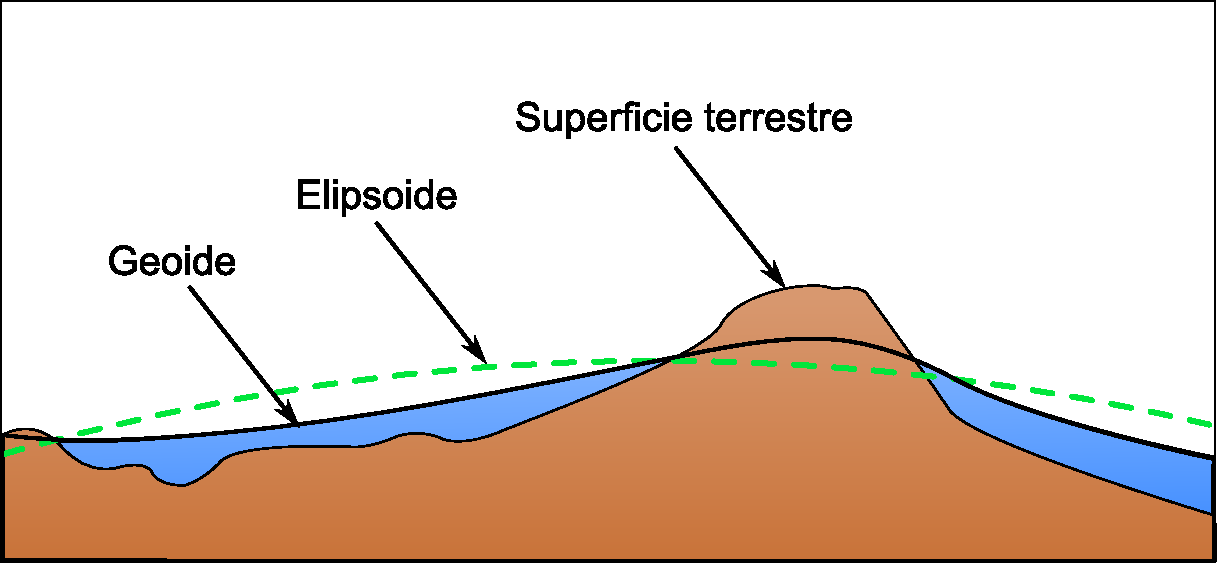
\includegraphics[width=.7\columnwidth]{Fundamentos_cartograficos/Tres_superficies.pdf}
\caption{\small Três superfícies fundamentais: superfície real da Terra, geoide e elipsoide (Adaptado da Wikipédia).}
\label{Fig:Tres_superficies} 
\end{figure}

Num elipsoide \textbf{global}, tanto o centro de gravidade quanto o plano equatorial coincidem com os da Terra. Já num elipsoide \textbf{local}, essas coincidências não são garantidas, sendo necessário mais informação sobre sua posição em relação à superfície terrestre.

Surge então o conceito de \textbf{datum}, que é a combinação de uma superfície de referência (elipsoide) e um ponto que o conecta ao geoide. Esse ponto é chamado de \textbf{ponto fundamental}, onde o elipsoide é tangente ao geoide. As verticais do geoide e do elipsoide coincidem nesse ponto.

Para um mesmo elipsoide, diferentes pontos fundamentais originam diferentes datums e, portanto, diferentes coordenadas para um mesmo ponto.

\subsection{Sistemas de coordenadas}

Após definir um modelo para a forma da Terra, podemos estabelecer um sistema para codificar posições em sua superfície e atribuir coordenadas a cada ponto. Há duas opções principais: utilizar \textbf{geometria esférica} para definir um sistema de coordenadas esféricas, ou utilizar \textbf{geometria plana}, o que exige uma \textbf{projeção cartográfica} da superfície curva para um plano.

O sistema de \textbf{coordenadas geográficas} é baseado em esferas, localizando pontos por meio de dois valores angulares: \textbf{latitude} e \textbf{longitude}. As linhas de mesma latitude e longitude são chamadas de \textbf{paralelos} e \textbf{meridianos}, respectivamente.

As coordenadas geográficas são muito úteis para grandes áreas, mas não constituem um sistema cartesiano. Tarefas como \textbf{medição de áreas ou distâncias} são complicadas com elas. Para facilitar tais operações e gerar cartografia, utilizamos coordenadas cartesianas, obtidas por meio da \textbf{projeção cartográfica}.

Como a superfície da esfera não é \textbf{desenvolvível} (isto é, não pode ser transformada em plano sem distorções), é necessário um método para converter seus pontos a um plano, conforme ilustra a Figura~\ref{Fig:Proyeccion}.

\begin{figure}
\centering
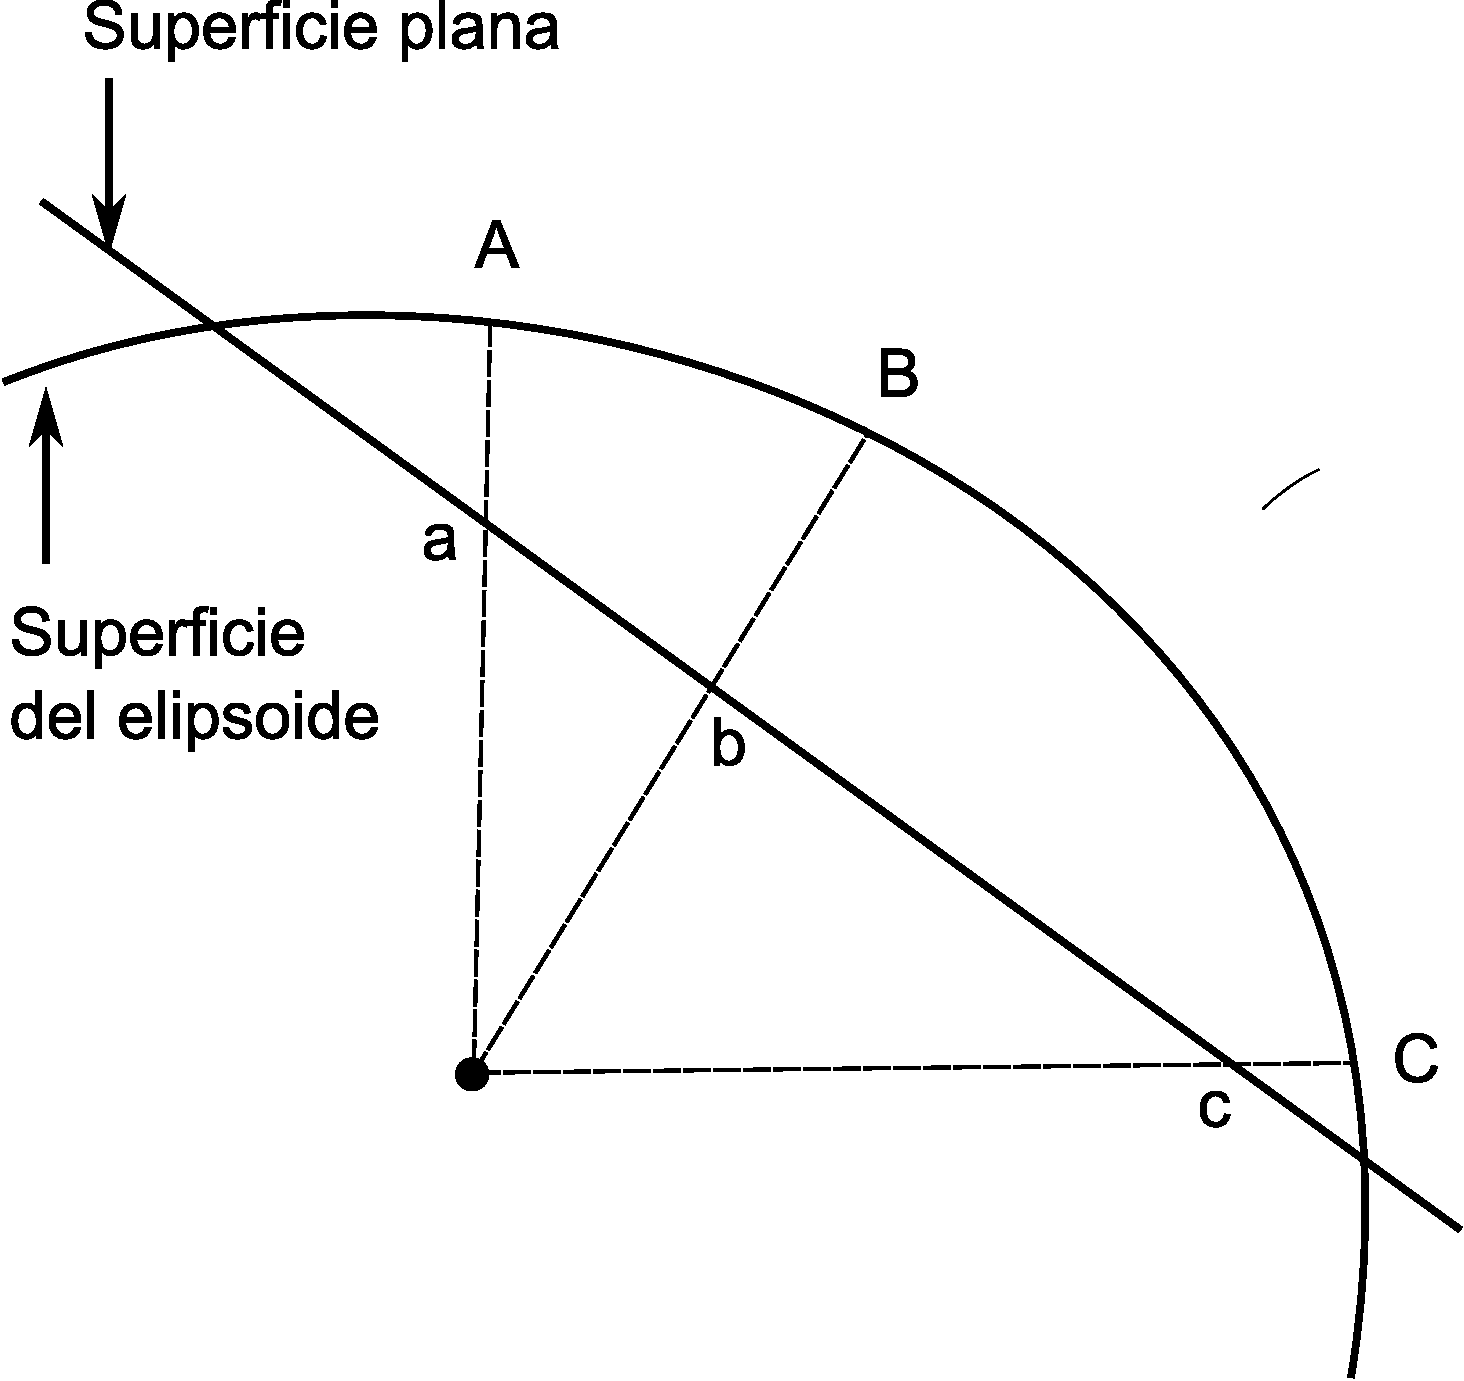
\includegraphics[width=.5\columnwidth]{Fundamentos_cartograficos/Proyeccion.pdf}
\caption{\small Esquema do conceito de projeção. Os pontos $A, B$ e $C$ na superfície do elipsoide têm equivalentes $a, b$ e $c$ no plano.}
\label{Fig:Proyeccion} 
\end{figure}

Além da projeção direta sobre um plano, pode-se usar superfícies desenvolvíveis, como cilindros ou cones, originando \textbf{projeções cônicas} ou \textbf{cilíndricas}.

Como mostra a figura, todas as projeções produzem \textbf{distorções}, chamadas de \textbf{anamorfoses}. A distância entre $A$ e $B$ na superfície não é igual à entre $a$ e $b$ no plano.

Conforme as propriedades métricas que preservam, as projeções podem ser:

\begin{itemize}
 \item \textbf{Equiárea} — preservam áreas;
 \item \textbf{Conformes} — preservam ângulos e formas;
 \item \textbf{Equidistantes} — preservam distâncias.
\end{itemize}

A escolha da projeção depende das \textbf{necessidades específicas} da aplicação.

Atualmente, uma das mais utilizadas é a \textbf{projeção transversa de Mercator}, que dá origem ao \textbf{sistema de coordenadas UTM}. Esse sistema divide a Terra em zonas e aplica parâmetros geodésicos específicos a cada uma. Usa o elipsoide WGS--84.

No sistema UTM, as coordenadas são expressas por meio de \textbf{zona + coordenadas relativas}. A Terra é dividida em 60 \textbf{fusos} de 6° de longitude cada, numerados de 1 a 60, de oeste para leste. Cada fuso é subdividido em 20 zonas latitudinais (C a X, exceto I e O), cada uma com 8° de latitude, exceto a zona X (12°).

As coordenadas são dadas em metros, com origem no cruzamento entre o meridiano central do fuso e o equador. Para evitar valores negativos, define-se a coordenada X inicial como 500.000 m, e a Y como 10.000.000 m (no hemisfério sul).

\subsection{Transformação e conversão de coordenadas}

É comum em SIG lidar com \textbf{diferentes sistemas de coordenadas} ou datums. Para unificar a informação, torna-se necessário \textbf{converter} os dados para um sistema comum. Se os datums forem diferentes, falamos em \textbf{transformação de coordenadas}.

SIGs oferecem funcionalidades para modificar as coordenadas dos dados geográficos ou para representá-los \textbf{em tempo real} em outro sistema (conversão \emph{on-the-fly}).

Sistemas de referência são padronizados com códigos. O mais comum é o \textbf{EPSG}.

\section{Conceitos cartográficos básicos}

Entre os conceitos fundamentais da cartografia destaca-se a \textbf{escala}, que expressa a \textbf{relação de tamanho} entre a representação no mapa e a realidade. Com ela, podemos converter medições do mapa em valores reais.

A escala é expressa como uma razão, por exemplo, 1:50.000 significa que 1 cm no mapa representa 500 m na realidade — isso é a \textbf{escala numérica}.

A escala só é exata em certas partes do mapa. Fora delas, varia. A razão entre a escala local e a numérica é o \textbf{fator de escala}.

Embora associada à representação, a escala também está ligada à \textbf{resolução dos dados} — ou seja, ao \textbf{tamanho mínimo cartografado} —, o que define a chamada \textbf{escala operacional} dos dados.

Em SIG, é possível aumentar a escala de visualização (\textbf{escala cartográfica}), mas isso não revela mais detalhes. Para isso, seria necessário coletar novos dados.

No caso de dados \emph{ráster}, o parâmetro relevante é o \textbf{tamanho da célula}, relacionado à escala.

O conceito de \textbf{generalização cartográfica} está ligado à representação simplificada de dados. É essencial para representar dados em escalas menores do que a escala de coleta. A Figura~\ref{Fig:Generalizacion_agregacion} mostra um exemplo.

\begin{figure}[!hbt]
\centering
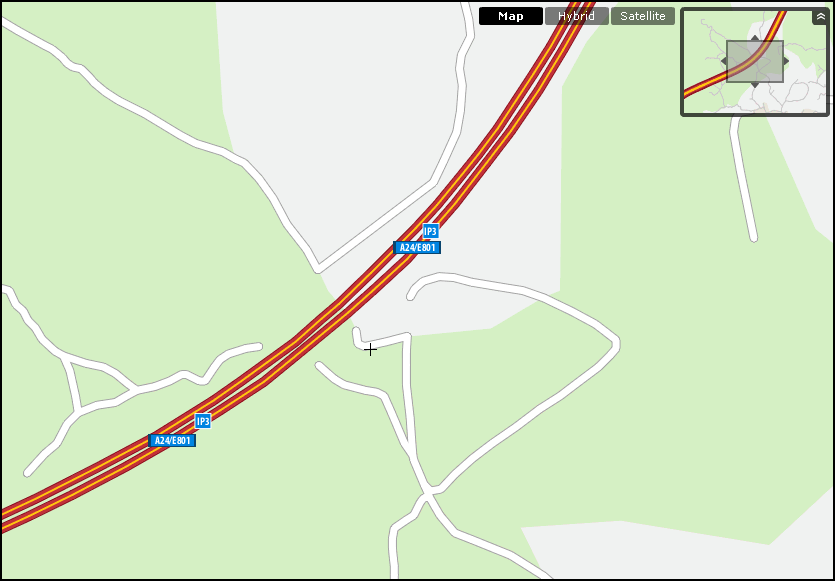
\includegraphics[width=.75\columnwidth]{Fundamentos_cartograficos/Generalizacion_agregacion.png}
\caption{\small Exemplo de generalização por agregação. Duas vias paralelas representadas como uma única via em escala menor (Fonte: Yahoo Maps).}
\label{Fig:Generalizacion_agregacion} 
\end{figure}

Outras operações de generalização incluem: 
\textbf{simplificação}, \textbf{agregação}, \textbf{exageração} (aumentar tamanho), e \textbf{deslocamento} (ajustar posição para legibilidade).

Em SIGs, a generalização pode ser feita em tempo real, mas isso consome muitos recursos e pode gerar resultados ruins.

Uma alternativa melhor é o uso de um \textbf{modelo multi-escalar} (Figura~\ref{Fig:SIG_multi_escala}), onde se mantém versões dos dados em diferentes escalas.

\begin{figure}[!hbt]
\centering
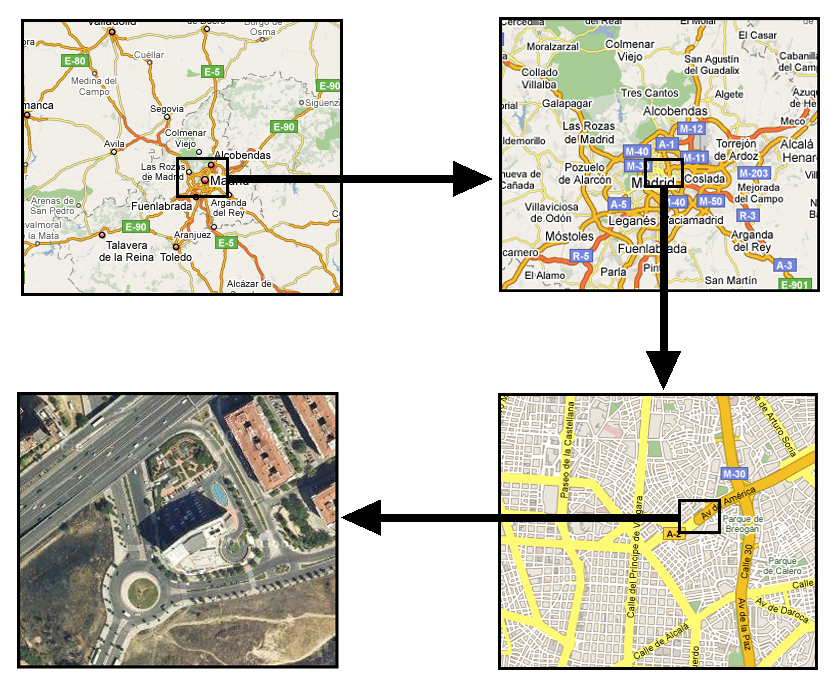
\includegraphics[width=\textwidth]{Fundamentos_cartograficos/SIG_multi_escala.png}
\caption{\small Em um SIG, é comum trabalhar com dados em diferentes escalas. A informação exibida depende da escala.}
\label{Fig:SIG_multi_escala} 
\end{figure}

O conceito de \emph{camada}, fundamental em SIGs, permite gerenciar dados em múltiplas escalas.

Para imagens, isso se traduz na criação de \textbf{pirâmides}, ou seja, conjuntos de imagens em diferentes resoluções, escolhidas conforme a escala de visualização.

\pagestyle{empty}

  %  \chapter{O dado geográfico e seu armazenamento}

De todos os subsistemas de um SIG, o relacionado aos dados é o pilar fundamental que impulsiona os demais. Os dados são o combustível que alimenta o SIG. Esse subsistema é também o mais inter-relacionado, estando inseparavelmente conectado a todos os outros.

\pagestyle{fancy}

\section{Dados e informação. Tipos de informação.}

Há uma diferença importante entre os conceitos de \textbf{dados} e \textbf{informação}. Um SIG é um Sistema de \emph{Informações} Geográficas, mas trabalha com \emph{dados} geográficos — conceitos distintos.

Dado é simplesmente um \textbf{conjunto de valores ou elementos} usados para representar algo. Por exemplo, o código 502132N é um dado.

Esse dado pode ser interpretado como uma coordenada geográfica (latitude 50\textdegree $21'$ $32''$ Norte) ou como um número de identificação. A informação muda, apesar de o dado ser o mesmo.

Assim, \textbf{informação é o resultado da interpretação de um dado}. O trabalho com dados visa, muitas vezes, extrair o máximo de informação possível.

Diferentes dados podem ter volumes diferentes mas conter a mesma informação. Por exemplo, os textos “502132NORTE” ou “CINQUENTA VINTE E UM TRINTA E DOIS NORTE” têm maior volume, mas expressam a mesma informação que “502132N”.

Na informação geográfica, distinguimos duas componentes: \textbf{espacial} (responde a "onde?") e \textbf{temática} (responde a "o quê?").

A componente espacial é geralmente numérica (coordenadas). Já a componente temática pode ser \textbf{numérica} ou \textbf{alfanumérica} (texto). Variáveis numéricas podem ser classificadas como:

\begin{itemize}
\item \textbf{Nominal}
\item \textbf{Ordinal}
\item \textbf{Intervalar}
\item \textbf{De razão}
\end{itemize}

O tipo de variável determina as operações possíveis em um SIG.

Outro conceito importante é a \textbf{dimensão} dos elementos (ponto = 0D, linha = 1D, polígono = 2D, volume = 3D), como mostrado na Figura~\ref{Fig:Dimensiones}.

\begin{figure}[!hbt] 
\centering
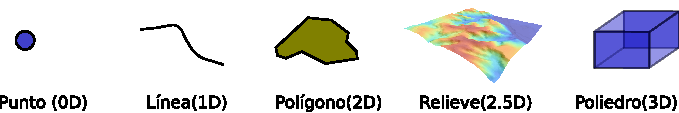
\includegraphics[width=\textwidth]{dados/Dimensiones.pdf}
\caption{\small Dimensões da componente geográfica.}
\label{Fig:Dimensiones} 
\end{figure}

\section{Divisão da informação: Camadas}

Em SIG, a informação espacial de uma região é \textbf{dividida em camadas} temáticas independentes (Figura~\ref{Fig:Concepto_capa}).

\begin{figure}[!hbt] 
\centering
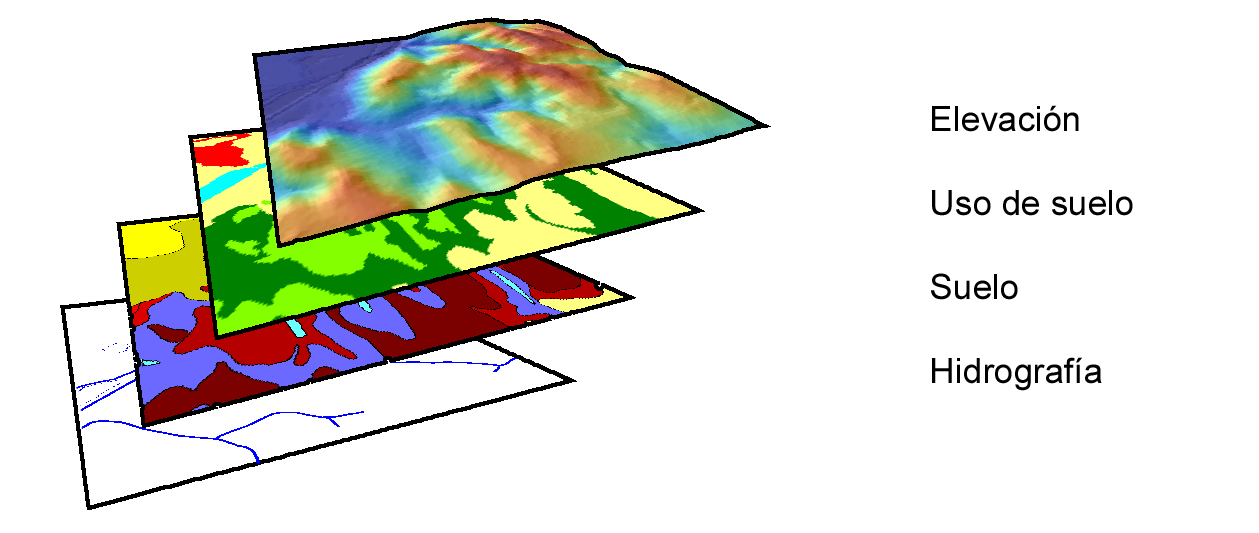
\includegraphics[width=\textwidth]{dados/Concepto_capa.png}
\caption{\small Conceito de \emph{camada} de informação geográfica em um SIG.}
\label{Fig:Concepto_capa} 
\end{figure}

O conceito de camada é essencial. Cada camada pode ser visualizada e manipulada separadamente. Diferentes tipos de informação são combinados facilmente, ao contrário da cartografia impressa.

Camadas também permitem versões de dados para diferentes escalas. Evitam redundância, já que cada camada armazena apenas um tipo de informação.

Além da divisão temática, os dados podem ser subdivididos espacialmente — como folhas de mapas impressos. A separação entre \textbf{dados e visualização} permite montar mosaicos a partir de diferentes fontes.

\section{Modelos de informação geográfica}

Transformar uma área geográfica em dados SIG envolve:

\begin{itemize}
\item \textbf{Modelo geográfico} — representação conceitual da realidade.
\item \textbf{Modelo de representação} — forma de descrever o modelo geográfico.
\item \textbf{Modelo de armazenamento} — estrutura para guardar os dados.
\end{itemize}

Os modelos de representação mais comuns em SIG são:

\begin{itemize}
\item \textbf{Raster}
\item \textbf{Vetorial}
\end{itemize}

\subsection{Modelo raster}

Divide o espaço em uma \textbf{malha regular} de células (Figura~\ref{Fig:Raster_closeup}).

\begin{figure}[!hbt]   
\centering
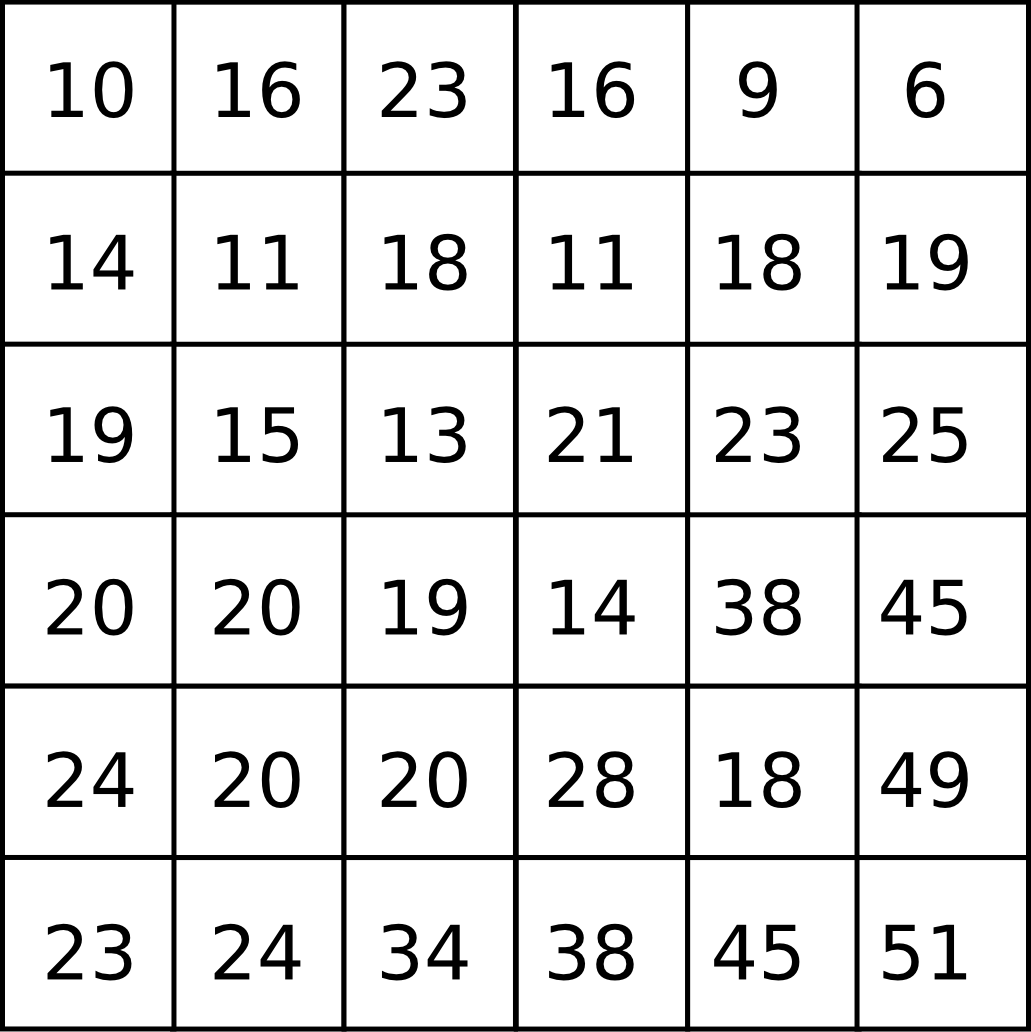
\includegraphics[width=.4\textwidth]{dados/Raster_closeup.png}
\caption{\small Células de uma malha raster com seus valores.}
\label{Fig:Raster_closeup} 
\end{figure}

Cada célula tem um valor numérico, geralmente em uma ou mais \textbf{bandas}. Imagens digitais e Modelos Digitais de Elevação (MDE) são exemplos de uso do modelo raster.

Cada raster pode ser tratado como uma \textbf{matriz}, facilitando análises matemáticas.

\subsection{Modelo vetorial}

Baseia-se em \textbf{entidades geométricas} (ponto, linha, polígono) — ver Figura~\ref{Fig:Primitivas_vectoriales}.

\begin{figure}[!hbt]   
\centering
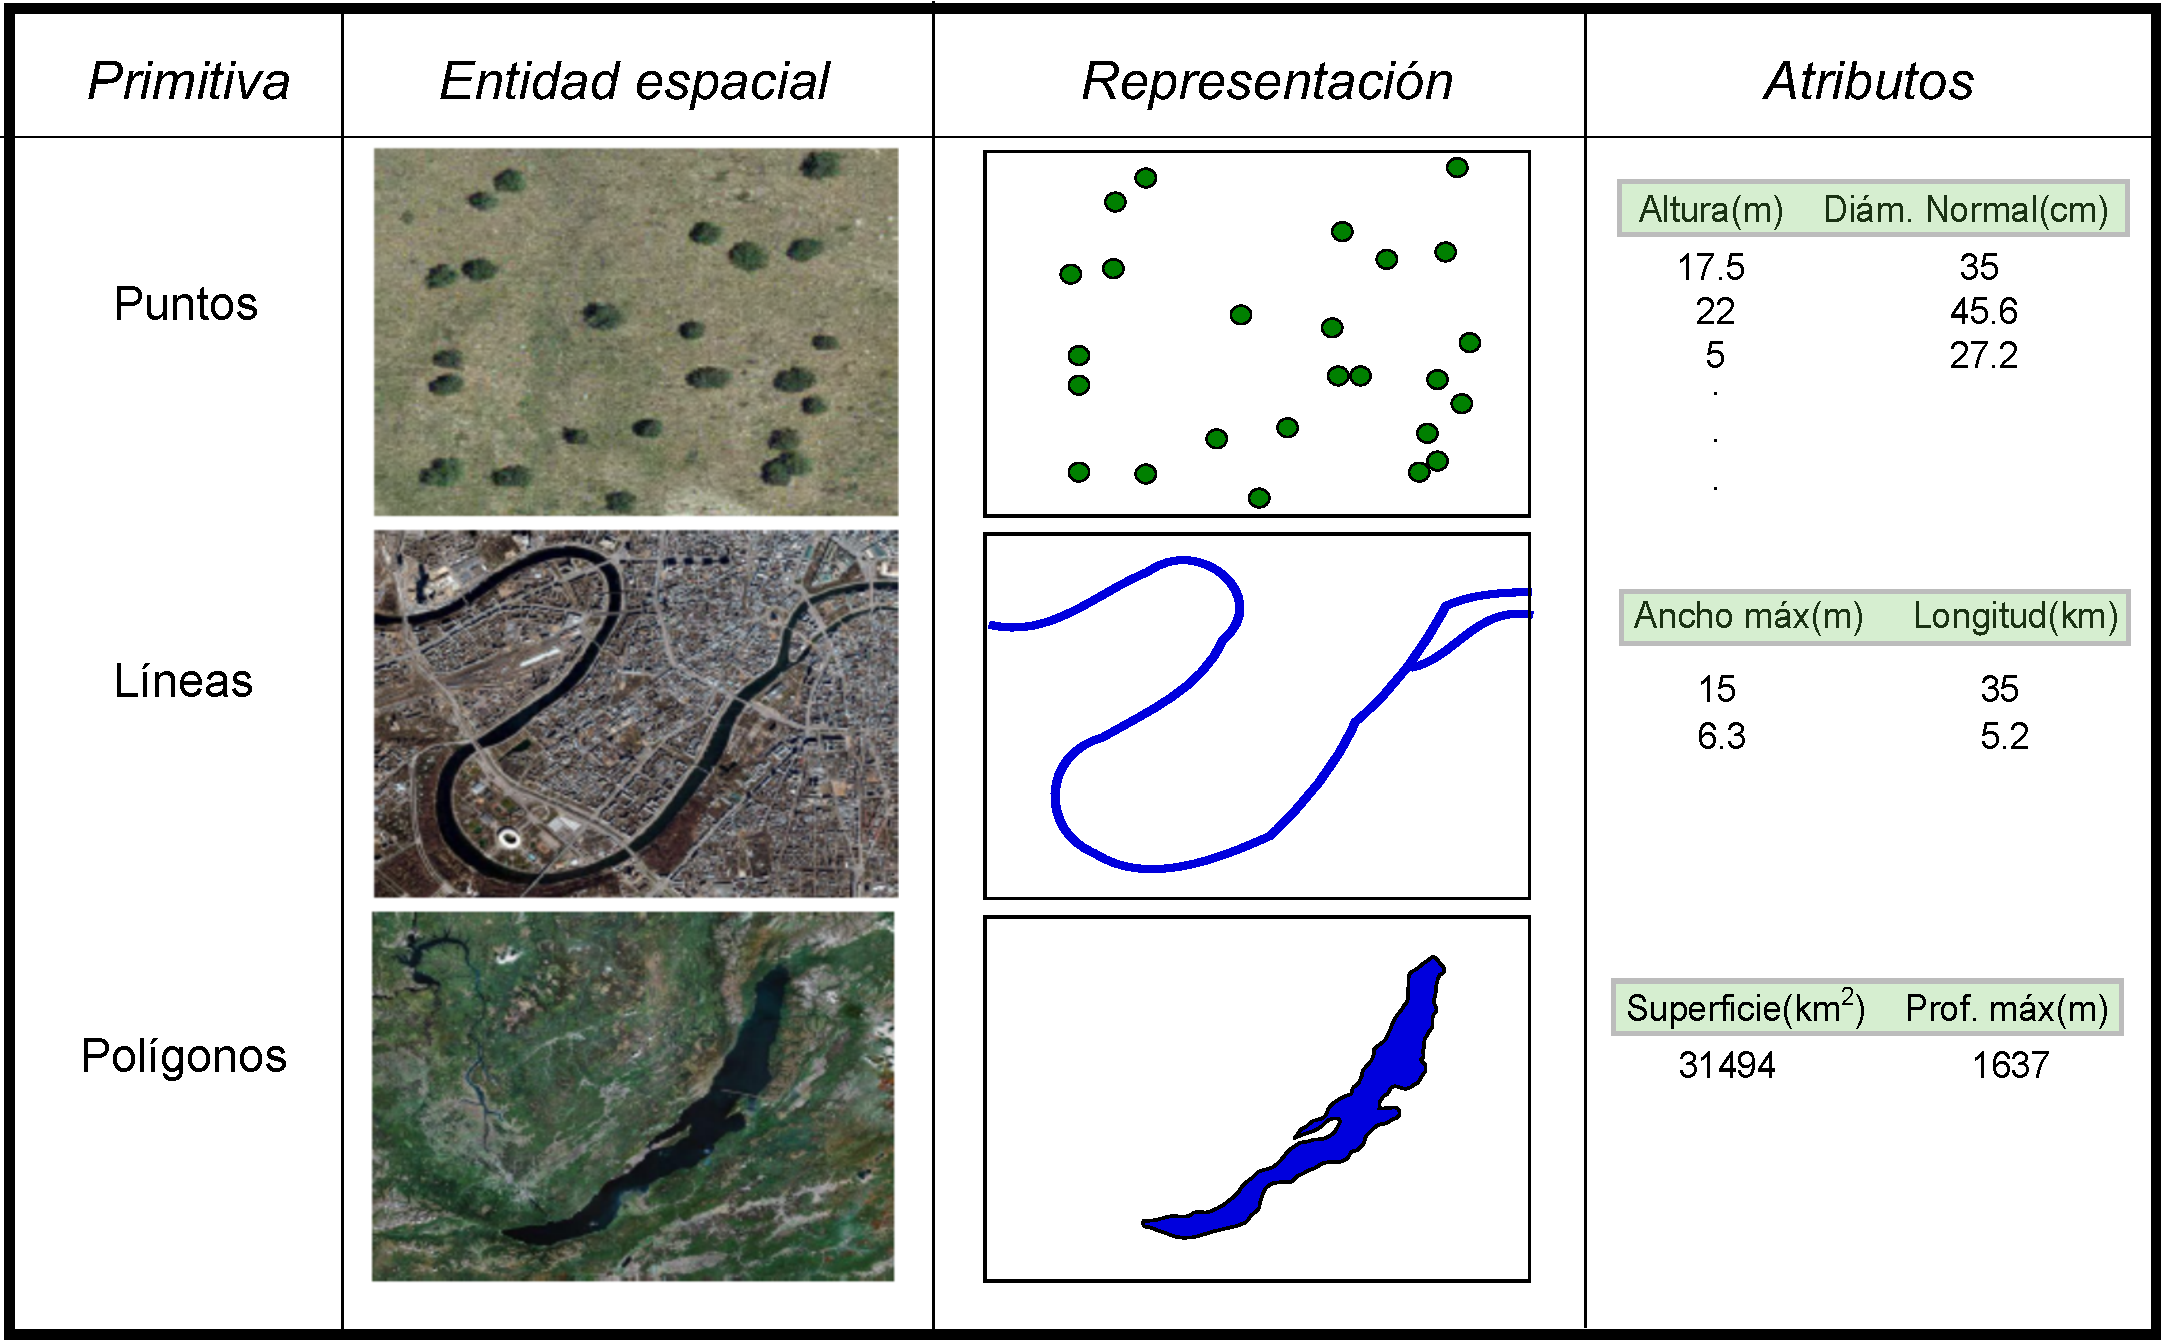
\includegraphics[width=\textwidth]{dados/Primitivas_vectoriales.pdf}
\caption{\small Primitivas geométricas e exemplos de atributos.}
\label{Fig:Primitivas_vectoriales} 
\end{figure}

Cada entidade pode ter múltiplas primitivas e diversos \textbf{atributos}, armazenados em tabelas (bancos de dados). Esses atributos podem ser analisados independentemente da geometria.

A \textbf{topologia} armazena relações espaciais entre entidades, sendo essencial em análises como redes viárias (Figura~\ref{Fig:Topologia_vias}).

\begin{figure}[!hbt]   
\centering
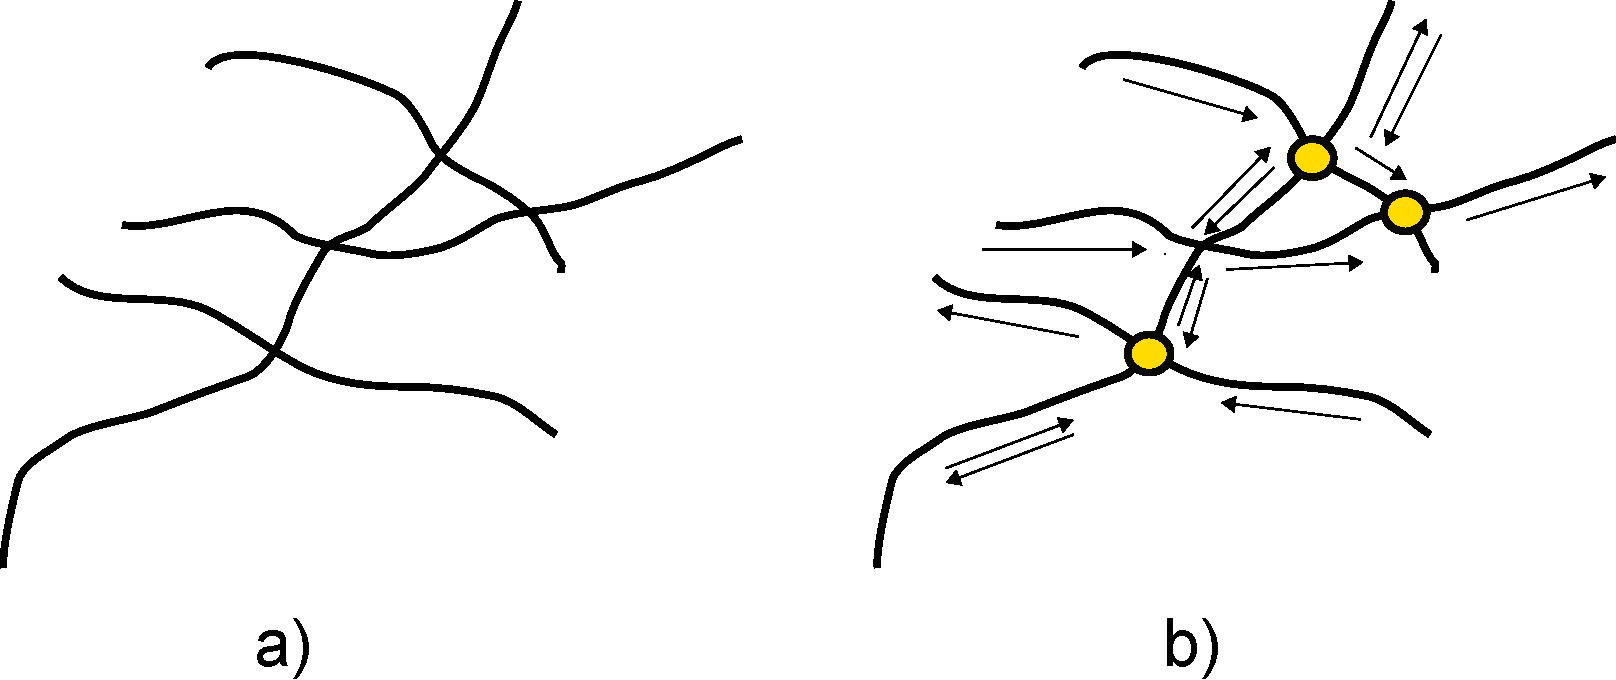
\includegraphics[width=.8\columnwidth]{dados/Topologia_vias.pdf}
\caption{\small Camada de vias sem (a) e com (b) topologia.}
\label{Fig:Topologia_vias} 
\end{figure}

Sem topologia, as entidades vetoriais são tratadas como um \emph{espaguete} — sem relações entre si.

\subsection{Raster \emph{vs} Vetorial}

Ambos os modelos podem representar qualquer tipo de informação (Figura~\ref{Fig:Esquemas_modelos_representacion}).

\begin{figure}[!hbt]   
\centering
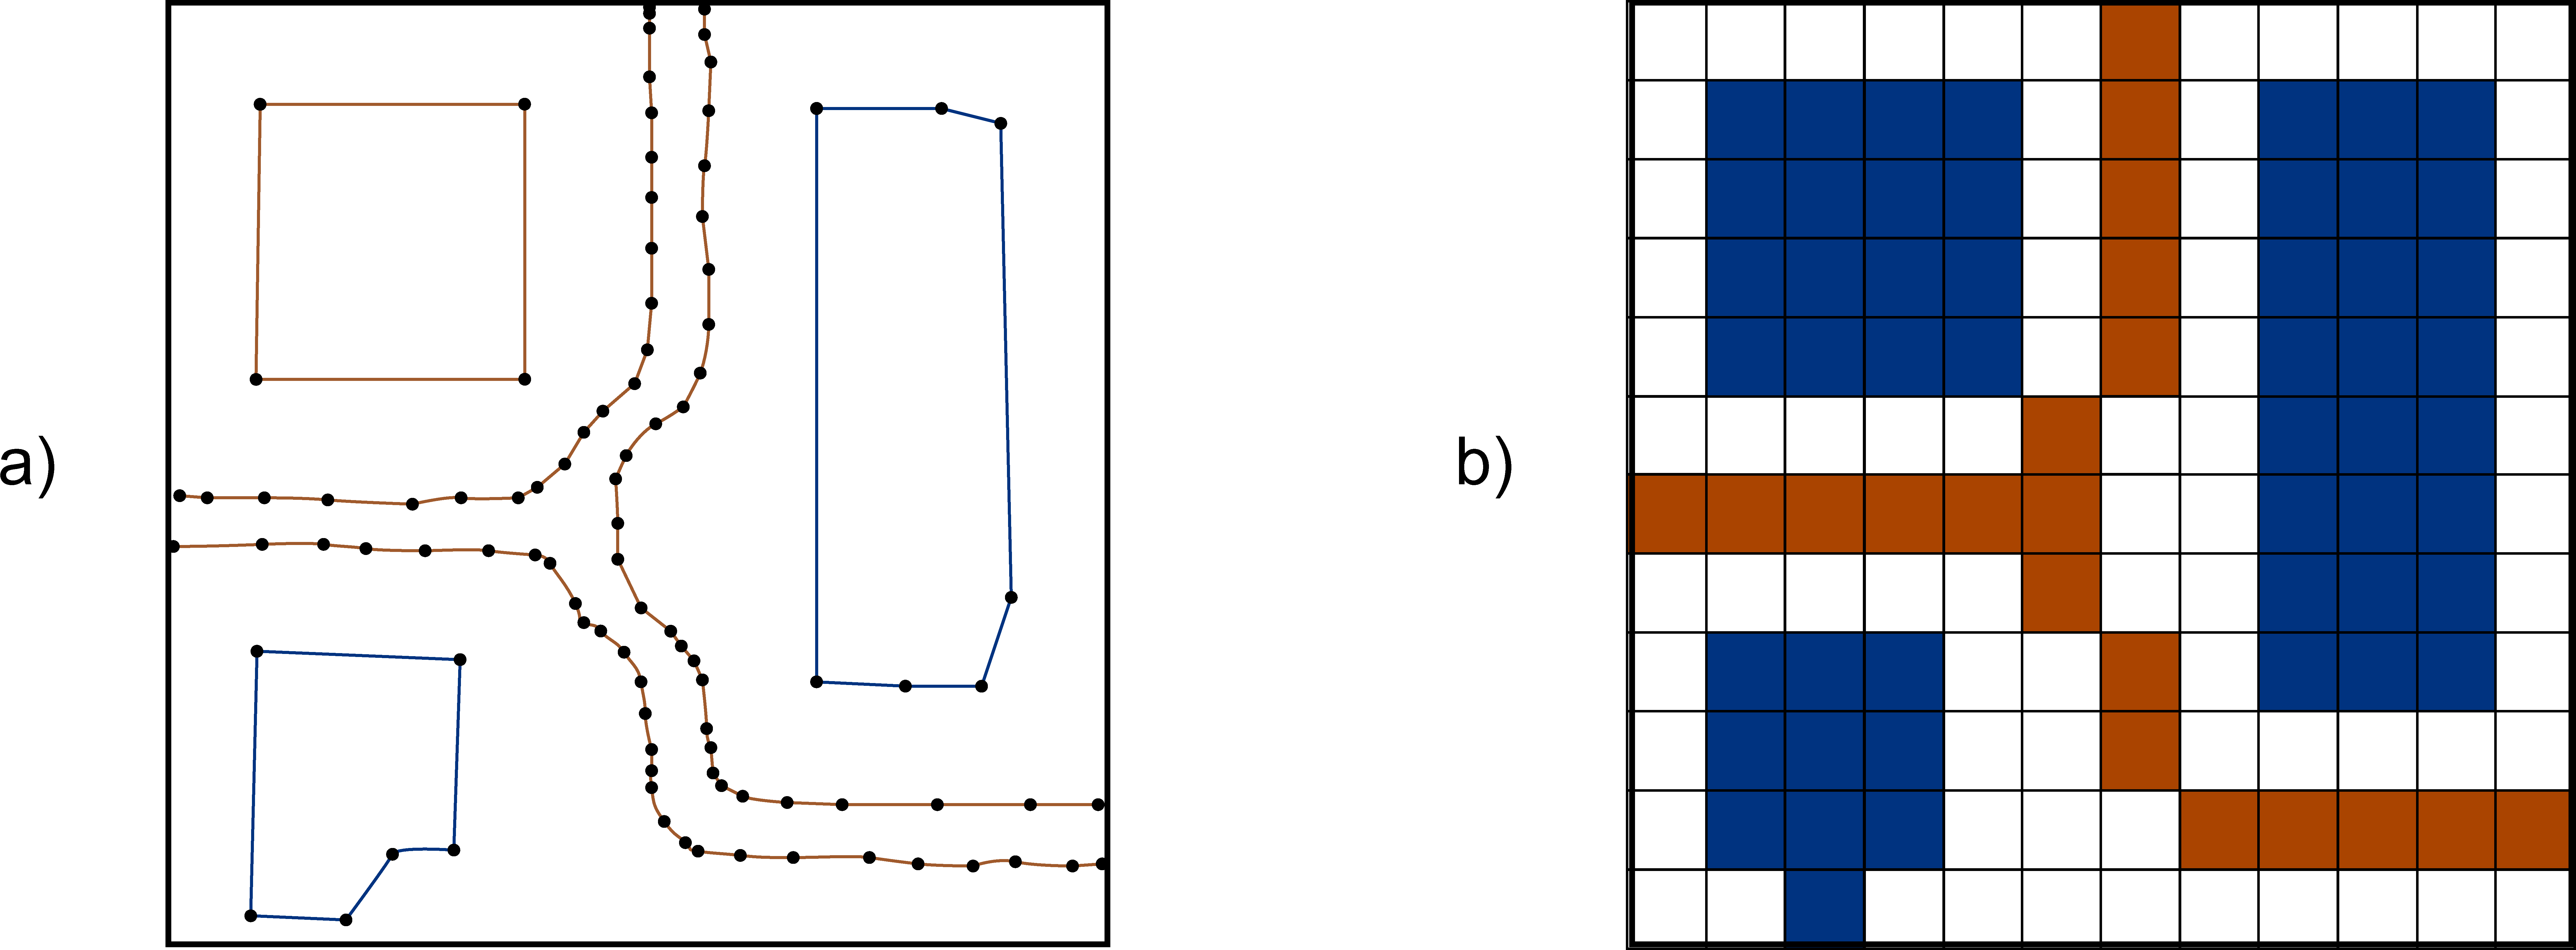
\includegraphics[width=\textwidth]{dados/Esquemas_modelos_representacion.pdf}
\caption{\small Comparação entre representação vetorial (a) e raster (b).}
\label{Fig:Esquemas_modelos_representacion} 
\end{figure}

Comparação:

\begin{itemize}
\item \textbf{Enfoque}: Raster enfatiza o \emph{o quê}, vetorial o \emph{onde}.
\item \textbf{Precisão}: Raster é limitado pelo tamanho da célula (Figura~\ref{Fig:Imprecision_raster}); vetorial tem maior precisão nas formas.

\begin{figure}[!hbt]   
\centering
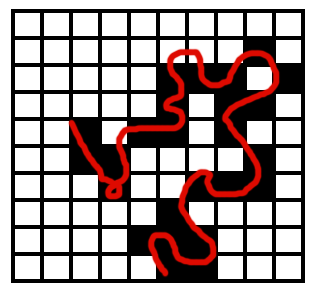
\includegraphics[width=.4\columnwidth]{dados/Imprecision_raster.png}
\caption{\small Limitação de forma no modelo raster.}
\label{Fig:Imprecision_raster} 
\end{figure}

\item \textbf{Complexidade}: Algoritmos de análise são mais fáceis de implementar em raster.
\end{itemize}

Não há modelo ideal absoluto. A escolha depende de:

\begin{itemize}
\item \textbf{Tipo de variável}: contínua (ex: elevação) → raster; discreta → vetorial.
\item \textbf{Tipo de análise}: raster para cálculos, vetorial para visualização.
\item \textbf{Contexto}: imagens sempre em raster.
\end{itemize}

É possível \textbf{converter} entre modelos conforme a necessidade da aplicação.

\pagestyle{empty}

  %  \chapter{Fontes principais de dados espaciais}

\pagestyle{fancy}

Até pouco tempo atrás, toda informação manipulada em um SIG tinha origem em um mapa em papel, que precisava ser \emph{preparado} para se adaptar à natureza digital do SIG. O dado geográfico era obtido por meio da \textbf{digitalização} da cartografia, ou seja, a conversão dos dados impressos em formato digital compatível com SIG.

Como aplicação computacional, um SIG depende exclusivamente de dados digitais. Os dados geográficos digitais oferecem várias vantagens em relação aos analógicos, além do simples fato de poderem ser incorporados ao SIG. Entre essas vantagens destacam-se: facilidade de atualização, distribuição simplificada (especialmente com a Internet), menor espaço de armazenamento físico, facilidade e precisão de análise, e manutenção eficiente (o dado digital não se degrada, apenas seu suporte, o que permite sua replicação sem perda de qualidade).

Atualmente, as técnicas de aquisição de dados evoluíram e permitem criar dados diretamente integráveis em um SIG. Assim, distinguimos \textbf{fontes primárias} e \textbf{fontes secundárias} de dados.

As \textbf{fontes primárias} geram dados que, em sua forma original, já podem ser utilizados em SIG, enquanto as \textbf{fontes secundárias} produzem dados que precisam de adaptação antes de serem usados.

Neste capítulo, exploraremos as diversas fontes de dados utilizáveis em um SIG.

\section{Sensoriamento remoto}\index{Sensoriamento remoto}

Sensoriamento remoto é o \textbf{estudo e medição das características de um objeto sem contato físico direto}. Mede-se, geralmente, a radiação eletromagnética refletida ou emitida pelos objetos na superfície terrestre.

Um sistema de sensoriamento remoto é composto pelos elementos da Figura~\ref{Fig:Elementos_teledeteccion}:

\begin{figure}[!hbt]   
\centering
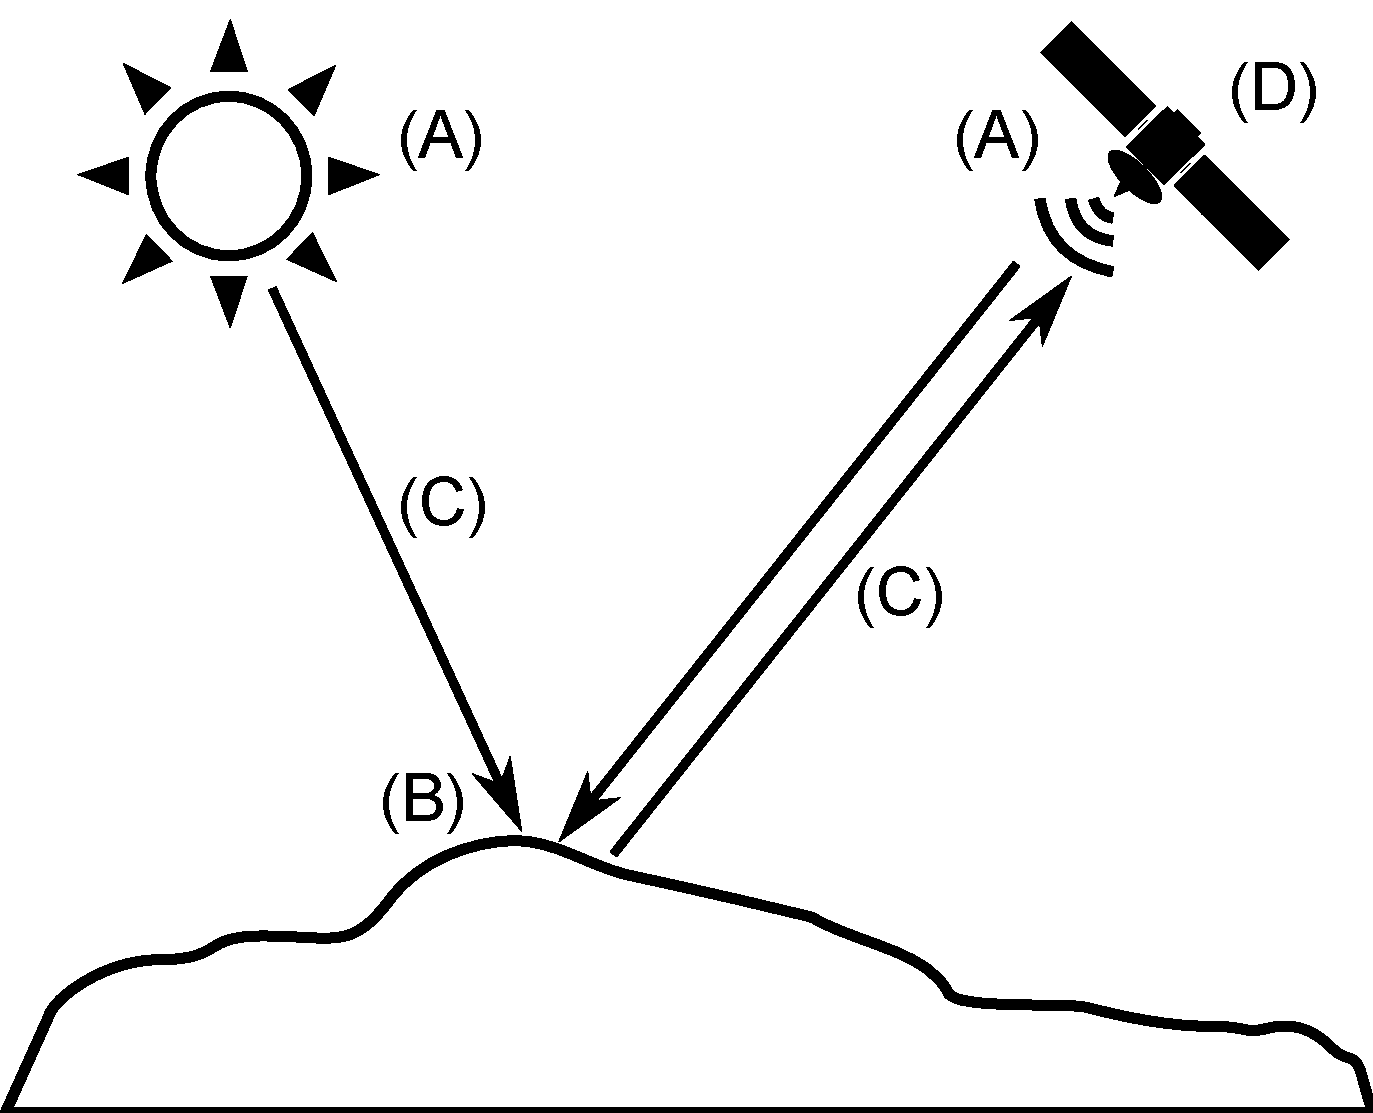
\includegraphics[width=.6\textwidth]{Fontes_dados/Elementos_teledeteccion.pdf}
\caption{\small Esquema de um sistema de sensoriamento remoto.}
\label{Fig:Elementos_teledeteccion} 
\end{figure}

\begin{itemize}
	\item \textbf{Fonte de radiação (A)}: natural ou artificial. A radiação interage com a superfície terrestre, sendo alterada por ela.
	\item \textbf{Objetos (B)}: refletem ou emitem radiação.
	\item \textbf{Atmosfera (C)}: atravessada pela radiação, podendo também alterá-la.
	\item \textbf{Receptor (D)}: capta a radiação refletida e gera uma imagem (camada raster), com valores de intensidade registrados em \textbf{Níveis Digitais} (geralmente entre 1 e 256).
\end{itemize}

A seguir, veremos detalhes desses elementos: fundamentos físicos (radiação e interação com a matéria) e análise dos receptores (sensores e plataformas).

\subsection{Fundamentos físicos}

A radiação eletromagnética resulta de alterações nos campos elétrico e magnético. Suas ondas propagam-se à velocidade da luz e são descritas por parâmetros como comprimento de onda e frequência. O conjunto dessas radiações compõe o \textbf{espectro eletromagnético}.

As principais interações dos objetos com a radiação são: \textbf{absorção, transmissão e reflexão}. Para o sensoriamento remoto, a \textbf{reflexão} é a mais relevante, pois é a radiação refletida que será captada para gerar imagens.

Cada objeto reflete radiações de diferentes comprimentos de onda de modo específico. Isso define sua \textbf{assinatura espectral}.

Imagens geradas possuem múltiplas bandas (valores por pixel), cada uma associada a uma faixa do espectro. Os Níveis Digitais em cada banda representam a intensidade da radiação naquela faixa específica.

\subsection{Sensores e plataformas}

Os principais elementos tecnológicos de um sistema de sensoriamento remoto são o \textbf{sensor} e a \textbf{plataforma}.

\begin{itemize}
\item \textbf{Sensores passivos} captam radiação natural (como a solar).
\item \textbf{Sensores ativos} emitem radiação (como radar e LiDAR) e captam sua reflexão.
\end{itemize}

O \textbf{LiDAR}, por exemplo, utiliza pulsos de laser e fornece dados sobre a \textbf{elevação}, sendo útil para mapear o relevo.

A \textbf{plataforma} é onde o sensor está instalado, podendo ser:
\begin{itemize}
\item \textbf{Atmosférica} (aviões) — oferecem flexibilidade de uso.
\item \textbf{Orbital} (satélites) — possuem órbitas definidas por parâmetros chamados de \textbf{parâmetros orbitais}.
\end{itemize}

Órbitas especiais incluem:
\begin{itemize}
\item \textbf{Geoestacionária} — acompanha a rotação da Terra.
\item \textbf{Heliossincrônica} — passa sempre pelo mesmo ponto à mesma hora solar.
\end{itemize}

\subsubsection{Resoluções}

Quatro tipos principais de resolução:

\begin{itemize}
\item \textbf{Espacial}: tamanho mínimo do objeto detectável (tamanho real do pixel).
\item \textbf{Espectral}: número e largura das bandas no espectro.
\item \textbf{Radiométrica}: profundidade dos Níveis Digitais (detalhe de intensidade).
\item \textbf{Temporal}: tempo entre duas aquisições de uma mesma área.
\end{itemize}

Nenhum sensor possui alta resolução em todos os aspectos. A escolha da imagem depende da aplicação.

\subsection{Fotogrametria}

Técnica que mede e define forma, dimensão e posição de objetos a partir de imagens, em especial \textbf{fotografias aéreas}. Utiliza \textbf{pares estereoscópicos} para criar \textbf{restituições 3D} do terreno.

Com imagens de satélite, pares são obtidos variando-se o \textbf{ângulo de visão} do sensor na mesma passagem.

Modalidades:
\begin{itemize}
\item \textbf{Analógica}
\item \textbf{Analítica}
\item \textbf{Digital} — base dos SIG.
\end{itemize}

Requer uma \textbf{estação fotogramétrica} digital com visualização estereoscópica, podendo incluir periféricos como \textbf{mouse 3D}.

\section{Cartografia impressa e digitalização}

Cartografia em papel (mapas, fotos antigas) precisa ser digitalizada para uso em SIG.

\begin{itemize}
\item \textbf{Raster}: via escaneamento.
\item \textbf{Vetorial}: exige registro geográfico, digitalização da geometria e dos atributos.
\end{itemize}

Digitalização pode ser:
\begin{itemize}
\item \textbf{Manual} — operador desenha entidades.
\item \textbf{Automática} — processo automatizado.
\end{itemize}

Dispositivos:

\begin{itemize}
\item \textbf{Tablet digitalizador}
\item \textbf{Editor SIG com mouse}
\end{itemize}

\textbf{Vectorização} é a digitalização automática para criar camadas vetoriais. A qualidade depende da preparação do documento.

Também é possível criar camadas a partir de \textbf{dados tabulares com coordenadas} (\textbf{geocodificação}). Se digitais, podem vir em planilhas, arquivos de texto, ou anexos de fotos (\emph{geotagging}).

\subsection{Qualidade da digitalização}

Erros podem surgir no processo, inclusive devido à fonte original (mapa degradado, linhas apagadas etc.). A Figura~\ref{Fig:Imprecisiones_digitalizacion} mostra exemplos.

\begin{figure}[!hbt]   
\centering
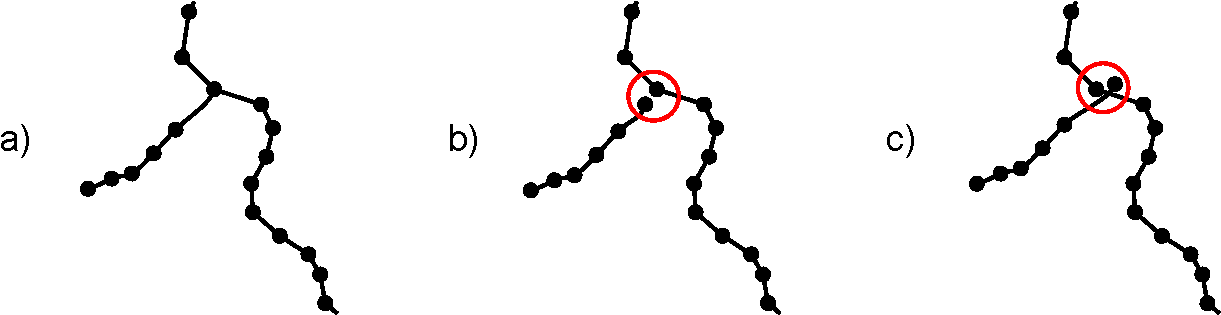
\includegraphics[width=\textwidth]{Fontes_dados/Imprecisiones_digitalizacion.pdf}
\caption{\small Erros na digitalização. a) Correto, b) e c) com nós desconectados.}
\label{Fig:Imprecisiones_digitalizacion} 
\end{figure}

SIGs modernos oferecem recursos de \textbf{snapping} e validação topológica para corrigir imprecisões durante a digitalização.

\section{GPS}

\textbf{Sistemas Globais de Navegação por Satélite (GNSS)} permitem determinar a posição de qualquer ponto na Terra com precisão de poucos metros.

O mais popular é o \textbf{GPS}, com 24 satélites operacionais. Usa \textbf{triangulação} e o datum \textbf{WGS84}.

Erros podem vir de:
\begin{itemize}
\item posição dos satélites,
\item reflexão do sinal,
\item interferência atmosférica,
\item imprecisão dos relógios.
\end{itemize}

\textbf{GPS diferencial} melhora a precisão usando um receptor fixo como referência. Isso permite alcançar:
\begin{itemize}
\item \textbf{2 m de precisão com correção}
\item \textbf{10–20 m sem correção}
\end{itemize}

Tipos de GPS:
\begin{itemize}
\item \textbf{Portátil} — para uso geral.
\item \textbf{Topográfico} — maior precisão e uso profissional.
\end{itemize}

Elementos coletados:
\begin{itemize}
\item \textbf{Waypoint} — ponto único.
\item \textbf{Track} — percurso contínuo.
\item \textbf{Route} — sequência de \emph{waypoints}.
\end{itemize}

\section{Informação Geográfica Voluntária (VGI)}

A \textbf{VGI} é a criação, gestão e compartilhamento de dados espaciais voluntários por usuários da Internet. Isso representa um \textbf{paradigma social e participativo}, rompendo com o monopólio estatal da cartografia.

Exemplo principal: \textbf{OpenStreetMap} (OSM).

Conceitos-chave:
\begin{itemize}
\item \textbf{Democratização da cartografia}
\item Cidadãos como \textbf{sensores ativos}
\item Redução do "mistério" da produção cartográfica
\end{itemize}

\section{Metadados}

\textbf{Metadados} são \textbf{dados sobre os dados}. Eles explicam, contextualizam e viabilizam o uso correto das informações geográficas.

Importância:
\begin{itemize}
\item Avaliar adequação dos dados.
\item Evitar uso indevido.
\item Facilitar busca, localização e catalogação.
\end{itemize}

Devem conter:
\begin{itemize}
\item \textbf{Identificação}
\item \textbf{Qualidade e linhagem dos dados}
\item \textbf{Componentes espaciais e temáticos}
\item \textbf{Distribuição e licenciamento}
\end{itemize}

Metadados podem ser:
\begin{itemize}
\item \textbf{Gerados na origem}
\item \textbf{Acrescentados depois} por distribuidores ou usuários
\end{itemize}

Formato:
\begin{itemize}
\item \textbf{Arquivos separados}
\item \textbf{Entradas em banco de dados}
\end{itemize}

\pagestyle{empty}

  %  \chapter{Software e tecnologia}

\pagestyle{fancy}

O conceito clássico de um SIG é o de uma aplicação completa que implementa ferramentas para realizar tarefas essenciais com dados geográficos: criação ou edição, manipulação e análise. Com o tempo, surgiram outras formas de aplicações que também se enquadram no âmbito dos SIG.

Neste capítulo, veremos as características dos aplicativos SIG, divididos em três grupos principais: ferramentas de desktop, cartografia na Web (\emph{Web mapping}) e SIG móvel. Também abordaremos aspectos tecnológicos relacionados.

\section{Ferramentas de desktop}

As funções básicas de um SIG de desktop podem ser divididas em cinco blocos: \textbf{entrada e saída de dados, visualização, edição, análise e geração de cartografia}. Um aplicativo de desktop geralmente possui todas essas funcionalidades, embora nem sempre com o mesmo nível de implementação.

\subsection{Entrada e saída de dados}

Um SIG de desktop deve ter capacidade para \textbf{ler} e, opcionalmente, \textbf{gravar dados}. A gravação é essencial quando o SIG permite gerar novas camadas. Em aplicações sem edição ou análise, essa funcionalidade pode não ser necessária.

Graças a bibliotecas e componentes de acesso a dados, os SIG de desktop podem lidar com \textbf{diversos formatos de dados}, ampliando sua \textbf{conectividade}.

Além de arquivos locais, é cada vez mais comum o acesso a \textbf{bancos de dados} e \textbf{serviços remotos}, que veremos adiante neste capítulo.

\subsection{Visualização}

Visualizar dados é uma função central dos SIG — essencial para interpretação, edição e análise. O ambiente visual se baseia em um \textbf{quadro de visualização} (ou canvas) no qual o usuário organiza camadas e ajusta a \textbf{simbologia} (forma de representação).

A ordem das camadas define a \textbf{hierarquia visual}. Ferramentas de navegação (zoom, pan) permitem explorar a visualização (Figura~\ref{Fig:Herramientas_navegacion}).

\begin{figure}[!hbt]
\centering
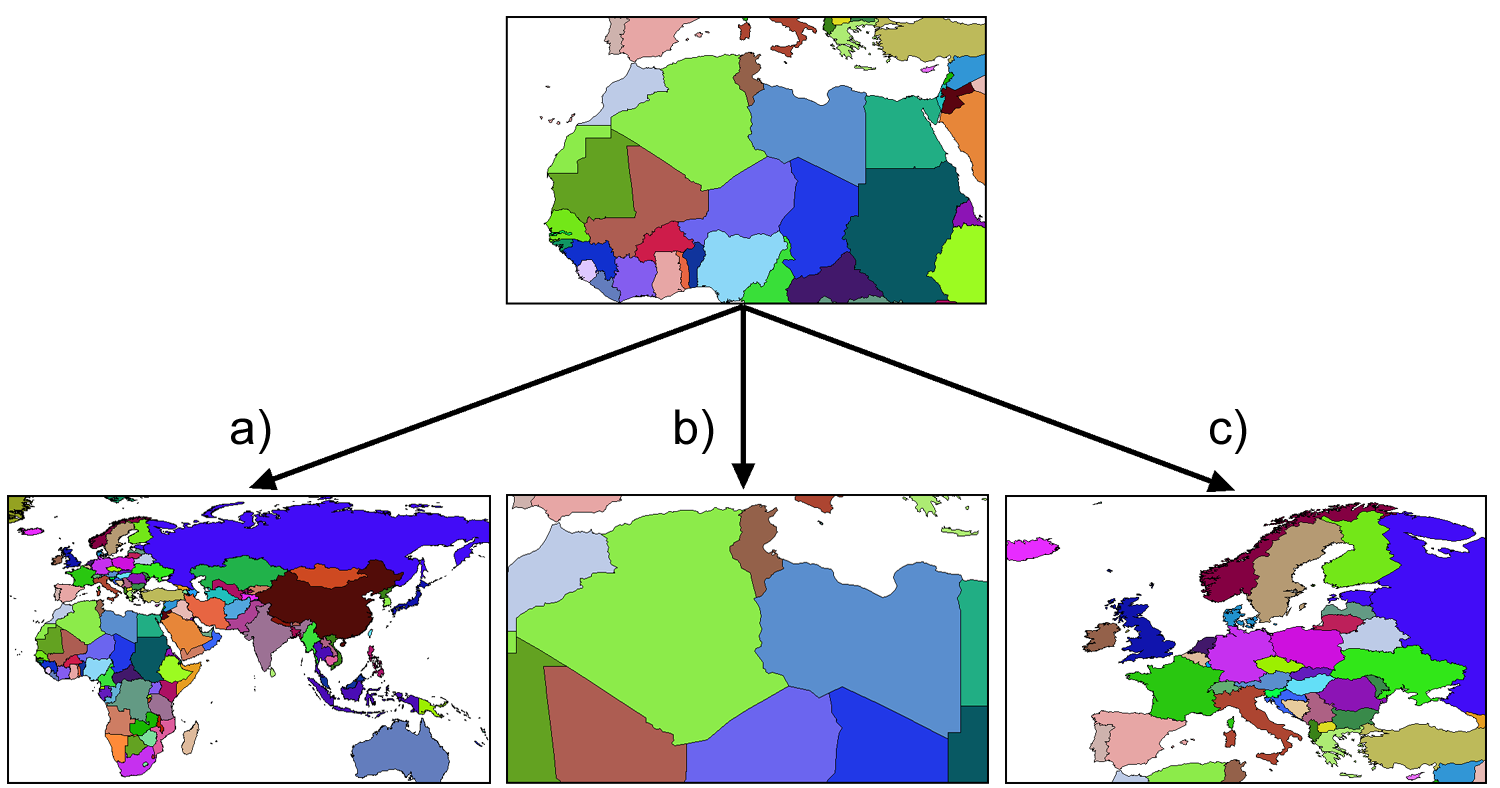
\includegraphics[width=.99\textwidth]{Software/Herramientas_navegacion.png}
\caption{\small Ferramentas básicas de navegação em um SIG de desktop: a) zoom out, b) zoom in, c) deslocamento (pan).}
\label{Fig:Herramientas_navegacion} 
\end{figure}

Diferente de mapas impressos, no SIG o usuário escolhe o que e como visualizar. Dados espaciais são \textbf{independentes de sua simbologia}, e podem ser representados de várias formas — especialmente vetoriais e ráster não visuais.

SIGs também podem ter \textbf{visualização tridimensional}, com controles adicionais para perspectiva, ângulos e relevo.

\subsection{Análise}

Desde o início dos SIG, a \textbf{análise} é uma das funções mais importantes.

Hoje, ferramentas de análise são vistas como \textbf{módulos} sobre uma plataforma base. Elas funcionam de forma \textbf{independente}, mas podem ser combinadas em fluxos de trabalho mais complexos.

Em análises interativas, o usuário interage com o visualizador (por exemplo, clicando num ponto) para fornecer parâmetros.

Na ausência de interação, os módulos funcionam como \textbf{processos automáticos} que recebem dados e retornam um resultado.

SIGs modernos permitem a \textbf{automação} de tarefas complexas por meio de \textbf{modelos de geoprocessamento}, combinando várias etapas em um fluxo.

Além disso, muitos SIG oferecem acesso via \emph{linguagens de script}, o que permite automatizar rotinas e personalizar análises mais sofisticadas.

\subsection{Edição}

Dados geográficos podem ser \textbf{modificados ou atualizados}. A edição é uma funcionalidade essencial em SIGs de desktop.

Podemos editar:

\begin{itemize}
 \item Geometrias vetoriais
 \item Atributos vetoriais
 \item Valores em camadas ráster
\end{itemize}

Ferramentas de edição são inspiradas em softwares CAD. Em alguns casos, também há suporte à edição com \textbf{topologia}.

\subsection{Geração de cartografia}

SIGs de desktop permitem \textbf{gerar mapas para impressão}, com controle sobre layout, legendas, escalas e outros elementos gráficos.

Eles incluem ferramentas para \textbf{automação cartográfica}, como modelos de impressão e geração de séries de mapas (Figura~\ref{Fig:Serie_mapas}).

\begin{figure}[!hbt]
\centering
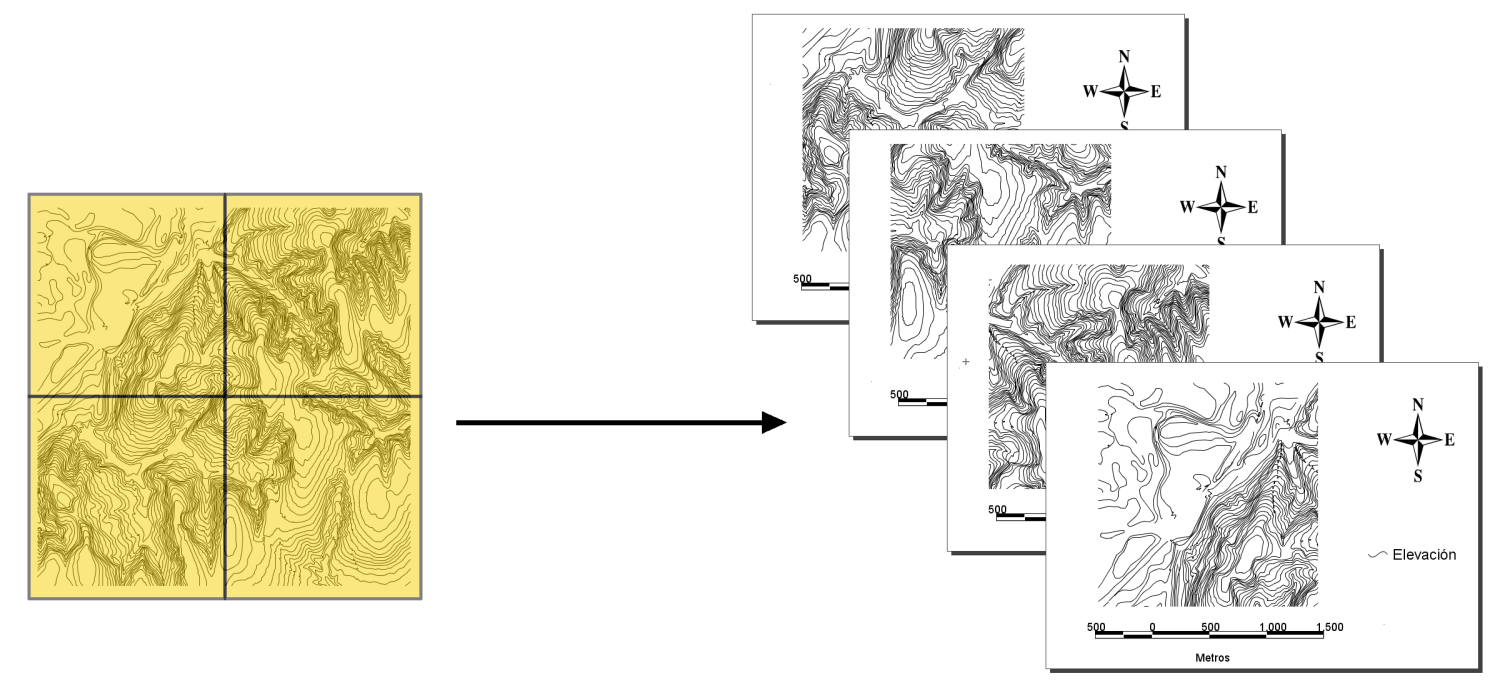
\includegraphics[width=\textwidth]{Software/Serie_mapas.png}
\caption{\small Automação de mapas: divisão de uma área em múltiplas páginas.}
\label{Fig:Serie_mapas} 
\end{figure}

Essa automação é possível porque os dados espaciais são \textbf{separados do design do mapa}.

\section{Cartografia na Web (\emph{Web Mapping}): clientes e servidores}

O \emph{Web Mapping} trouxe os SIG para o ambiente Web. Usa o navegador como plataforma e se baseia na \textbf{arquitetura cliente–servidor}.

O \textbf{servidor} armazena e fornece os dados. O \textbf{cliente} (navegador, app etc.) solicita e usa esses dados.

Exemplo de endereço Web:

\begin{center}
\small\texttt{http://victorolaya.com/writing}
\end{center}

Estrutura:

\begin{itemize}
 \item \texttt{http} — protocolo
 \item \texttt{victorolaya.com} — servidor
 \item \texttt{writing} — recurso (página)
\end{itemize}

Funcionamento básico:

\begin{enumerate}
 \item Cliente faz a requisição
 \item Ela é enviada pela rede até o servidor
 \item O servidor retorna os dados (ou erro)
 \item O cliente renderiza o resultado
\end{enumerate}

Ver Figura~\ref{Fig:Asi_funciona_internet}.

\begin{figure}[!hbt]   
\centering
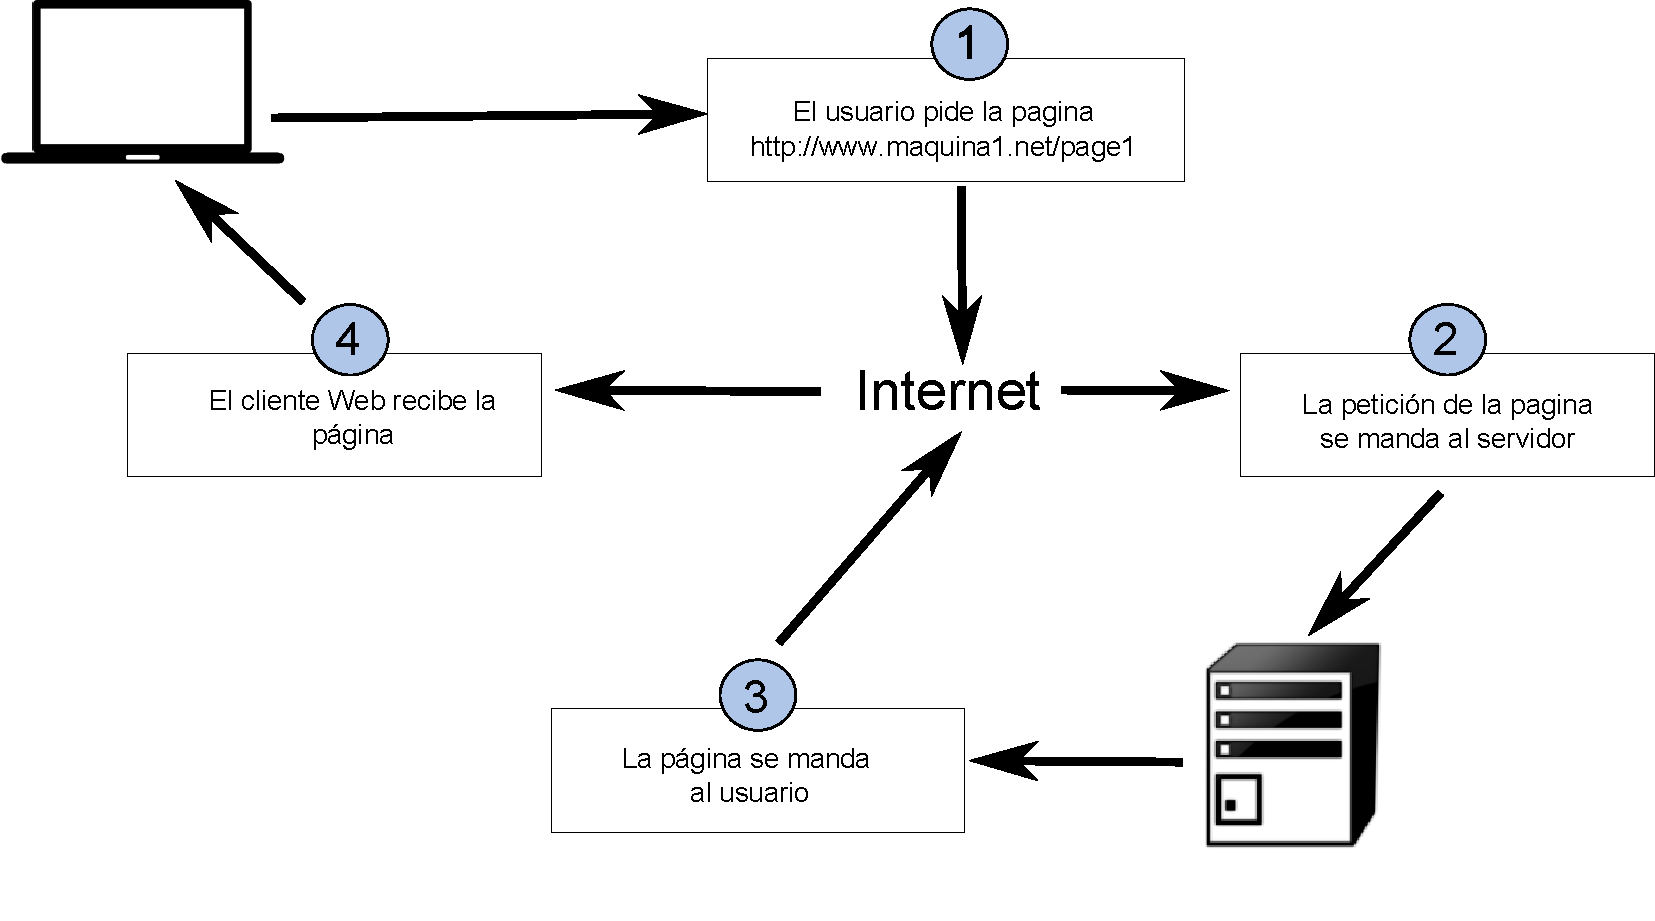
\includegraphics[width=\columnwidth]{Software/Asi_funciona_internet.pdf}
\caption{\small Funcionamento da Web: cliente e servidor.}
\label{Fig:Asi_funciona_internet} 
\end{figure}

Serviços SIG baseados em servidor:

\begin{itemize}
 \item \textbf{Representações gráficas}: imagens geradas pelo servidor
 \item \textbf{Dados brutos}: o cliente recebe os dados e faz a representação ou análise
 \item \textbf{Consultas}: o cliente faz perguntas, e o servidor responde com subconjuntos ou metadados
 \item \textbf{Processos remotos}: o servidor executa análises ou cálculos e retorna os resultados (ver Figura~\ref{Fig:Datos_y_procesos_remotos})
\end{itemize}

\begin{figure}[!hbt]   
\centering
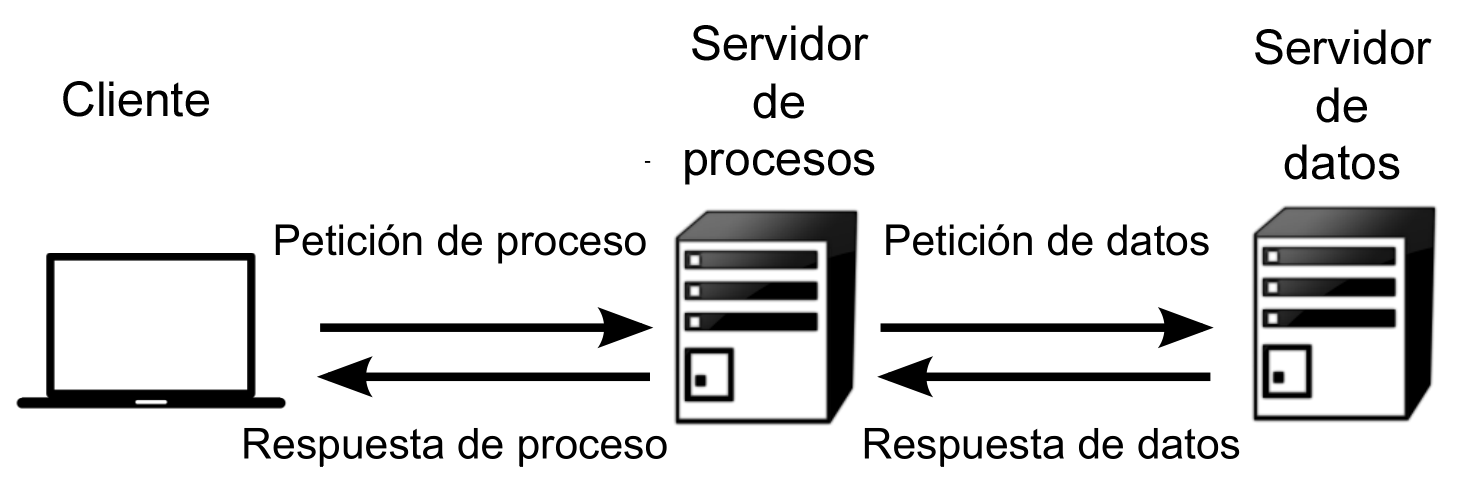
\includegraphics[width=0.95\textwidth]{Software/Datos_y_procesos_remotos.png}
\caption{\small Processamento remoto com acesso a dados em outros servidores.}
\label{Fig:Datos_y_procesos_remotos} 
\end{figure}

Tipos de clientes:

\begin{itemize}
 \item \textbf{Cliente pesado}: software completo (ex: SIG de desktop)
 \item \textbf{Cliente leve}: Web mapping em navegador; simples, mas cada vez mais avançado
\end{itemize}

SIGs Web mais modernos oferecem funcionalidades como edição de camadas, análise e acesso a serviços — formando o chamado \textbf{Web GIS}.

\section{Técnicas para serviços SIG: \emph{Tiling} e \emph{Cache}}

\index{Tiling}\index{Cache}

Essas técnicas são aplicadas principalmente em clientes Web que usam imagens.

\begin{itemize}
 \item \textbf{Tiling}: divide a imagem em mosaicos menores (teselas), otimizando o carregamento
 \item \textbf{Cache}: armazena localmente as teselas já carregadas, evitando downloads repetidos
\end{itemize}

Ver Figura~\ref{Fig:Tiling} para exemplo de economia de dados ao movimentar o mapa.

\begin{figure}[!hbt]   
\centering
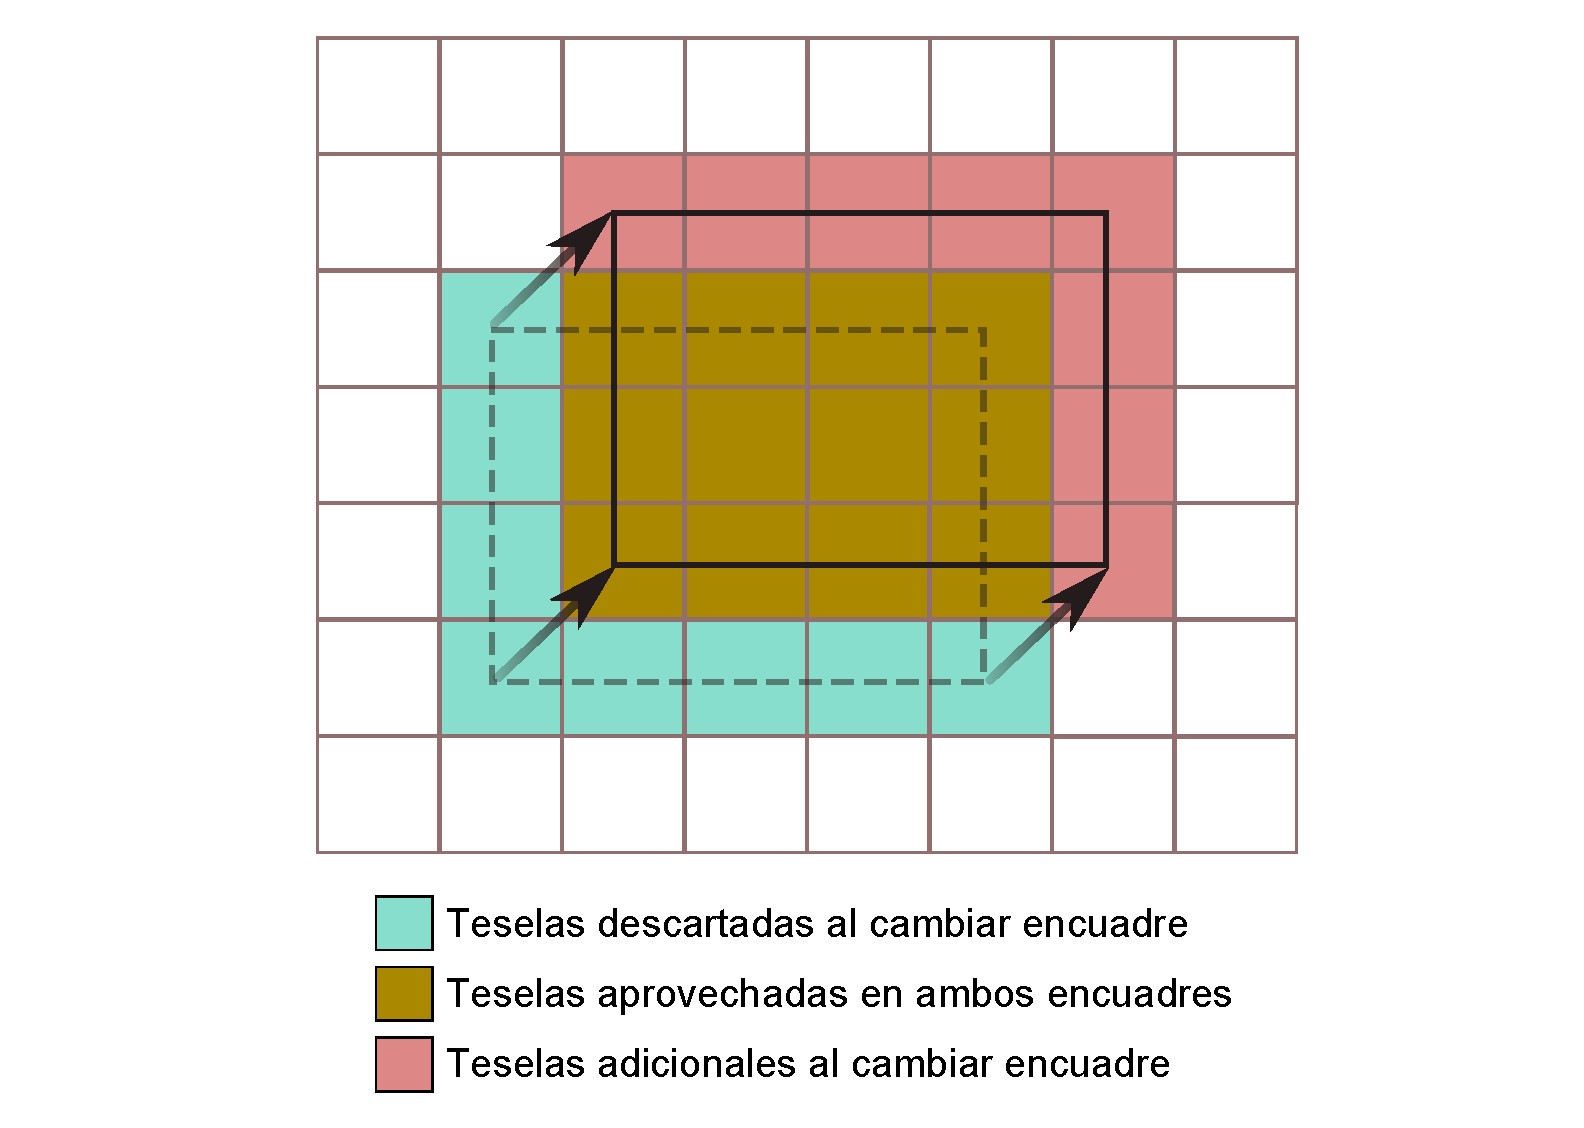
\includegraphics[width=\textwidth]{Software/Tiling.pdf}
\caption{\small Uso combinado de \emph{tiling} e \emph{cache} em um cliente SIG Web.}
\label{Fig:Tiling} 
\end{figure}

Outra técnica recente: \textbf{tiling vetorial}, onde:

\begin{itemize}
 \item Envia-se apenas os dados vetoriais da região visível
 \item O cliente aplica a simbologia localmente
\end{itemize}

Vantagens:

\begin{itemize}
 \item Menor volume de dados
 \item Transições suaves ao mudar de escala
\end{itemize}

\section{Padrões}

Para funcionar corretamente, o sistema cliente–servidor precisa de \textbf{padrões abertos} que garantam \textbf{interoperabilidade}.

Padrões garantem que diferentes sistemas possam se comunicar mesmo se desenvolvidos por fornecedores distintos.

Tipos:

\begin{itemize}
 \item \textbf{De fato} — aceitos na prática
 \item \textbf{De jure} — formalizados por instituições (ex: ISO)
 \item \textbf{Abertos} — disponíveis publicamente, gratuitos e neutros
\end{itemize}

Ver Figura~\ref{Fig:Esquema_no_interoperable} (sem padrões) e Figura~\ref{Fig:Esquema_interoperable} (com padrões).

\begin{figure}[!hbt]   
\centering
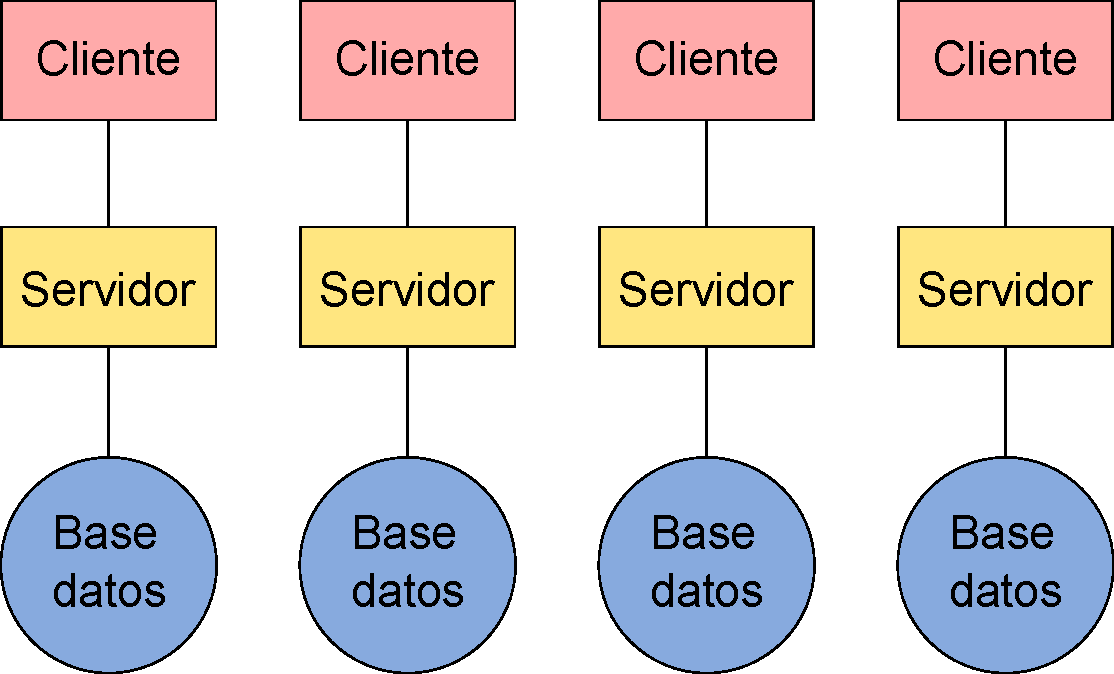
\includegraphics[width=.7\columnwidth]{Software/Esquema_no_interoperable.pdf}
\caption{\small Arquitetura não interoperável.}
\label{Fig:Esquema_no_interoperable} 
\end{figure}

\begin{figure}[!hbt]   
\centering
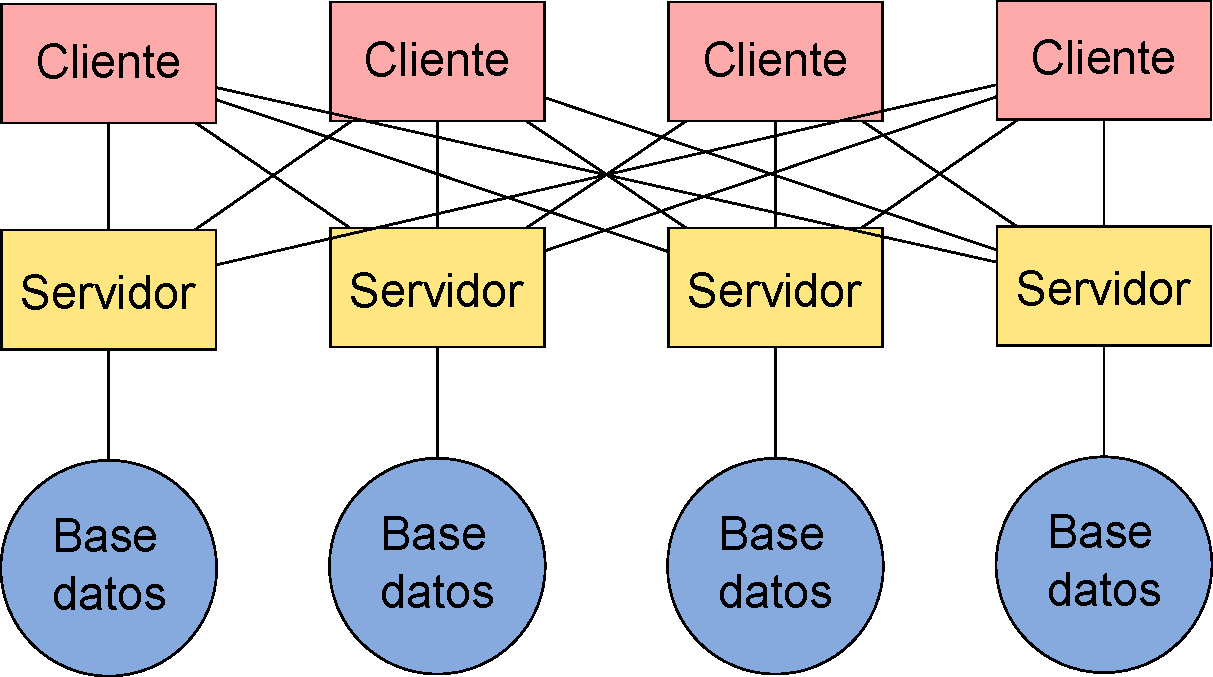
\includegraphics[width=.7\columnwidth]{Software/Esquema_interoperable.pdf}
\caption{\small Arquitetura interoperável baseada em padrões abertos.}
\label{Fig:Esquema_interoperable} 
\end{figure}

Desvantagens da falta de interoperabilidade:

\begin{itemize}
 \item Redundância de dados e alto custo
 \item Múltiplos clientes necessários
 \item Dados e funcionalidades não podem ser combinados
\end{itemize}

\subsection{Principais padrões}

Desenvolvidos pelo \textbf{Open Geospatial Consortium (OGC)}:

\begin{itemize}
 \item \textbf{WMS}: imagens de mapas
 \item \textbf{WCS}: camadas ráster
 \item \textbf{WFS}: camadas vetoriais
 \item \textbf{WPS}: serviços de processamento
 \item \textbf{GML}: formato para armazenamento
 \item \textbf{CSW}: consulta em catálogos
\end{itemize}

Outros padrões relevantes:

\begin{itemize}
 \item \textbf{ISO}: formatos e metadados
 \item \textbf{W3C}: comunicação na Web
\end{itemize}

\section{SIG móvel}

SIGs móveis (celulares, tablets) combinam elementos do SIG tradicional com as funcionalidades dos dispositivos móveis.

Funcionalidades principais:

\begin{itemize}
 \item \textbf{Acesso à Internet}
 \item \textbf{Posicionamento} (manual, via rede ou GPS)
\end{itemize}

Mesmo com limitações, SIGs móveis possibilitam:

\begin{itemize}
 \item \textbf{Coleta de dados em campo}
 \item \textbf{Navegação baseada em localização}
 \item \textbf{Serviços contextuais}
\end{itemize}

Aplicações:

\begin{itemize}
 \item \textbf{Navegação}
 \item \textbf{Inventário geográfico}
 \item \textbf{Guias e informações locais}
 \item \textbf{Publicidade geolocalizada}
 \item \textbf{Monitoramento de pessoas ou objetos}
 \item \textbf{Gestão de ativos ou frotas}
\end{itemize}

Sensores embutidos (GPS, bússola, acelerômetro, luz etc.) expandem as possibilidades do SIG móvel.

\pagestyle{empty}

  %  \chapter{Bancos de dados}

\pagestyle{fancy}

Os bancos de dados são elementos fundamentais no ambiente computacional atual, com aplicação praticamente universal. Concebidos para um propósito geral, são úteis em qualquer disciplina que exija a gestão de dados — especialmente quando esses dados são volumosos.

No caso dos SIG, a quantidade de dados cresce constantemente, tanto em volume quanto em precisão. Além disso, há características específicas como múltiplos usos, necessidade de acesso eficiente e indexação, que recomendam o uso de bancos de dados e tecnologias próprias para sua gestão.

Entendemos por \emph{banco de dados} um \textbf{conjunto de dados estruturado e armazenado sistematicamente}, com o objetivo de facilitar seu uso posterior. A chave está na \textbf{estrutura} e \textbf{sistematização}, que tornam o banco de dados superior a uma simples coleção desorganizada de arquivos.

As vantagens diretas do uso de um banco de dados incluem:

\begin{itemize}
	\item \textbf{Maior independência}: os dados são independentes das aplicações e dos usuários.
	\item \textbf{Maior disponibilidade}: acesso facilitado a partir de diferentes sistemas e locais.
	\item \textbf{Maior segurança}: replicação e sincronização de dados mais confiáveis.
	\item \textbf{Menor redundância}: menos dados repetidos, maior rapidez.
	\item \textbf{Maior eficiência na entrada e codificação de dados}.
\end{itemize}

Isso se reflete diretamente nos resultados:

\begin{itemize}
	\item \textbf{Maior coerência}: melhor gestão → melhor qualidade dos dados.
	\item \textbf{Maior eficiência}: acesso rápido aos dados.
	\item \textbf{Maior valor informativo}: facilita a extração de informação relevante.
\end{itemize}

Para os usuários:

\begin{itemize}
	\item \textbf{Facilidade de acesso}: basta saber utilizar os dados, não gerenciá-los.
	\item \textbf{Reutilização de dados}: maior compartilhamento.
\end{itemize}

Resumidamente, a principal qualidade de um banco de dados é a \textbf{centralização} dos dados — o que melhora o gerenciamento, a estrutura e o acesso.

\section{Bancos de dados relacionais}

O modelo mais comum, tanto em SIG quanto em outras áreas, é o de \textbf{bancos de dados relacionais}, baseado em \textbf{tabelas}.

Cada tabela (ou \textbf{relação}) possui:

\begin{itemize}
 \item \textbf{Registros} (linhas)
 \item \textbf{Campos} (colunas)
\end{itemize}

Cada linha, chamada de \textbf{tupla}, representa uma entidade com atributos distintos.

Um banco de dados geralmente contém múltiplas tabelas interligadas. Para isso, utilizamos os \textbf{atributos-chave}, que são \textbf{únicos e invariáveis} para cada entidade (ex: número de CPF).

Em dados espaciais, a \textbf{geometria} pode ser usada como chave.

Relações entre tabelas podem ser:

\begin{itemize}
 \item \textbf{Um para um}
 \item \textbf{Um para muitos}
 \item \textbf{Muitos para muitos}
\end{itemize}

Exemplo: uma pessoa pode morar em uma cidade, mas uma cidade pode ter muitas pessoas.

\section{Sistemas gerenciadores de banco de dados (SGBD)}

O SGBD (ou DBMS — \emph{Database Management System}) é o \textbf{intermediário entre os dados e os aplicativos}, como o SIG.

Funções do SGBD:

\begin{itemize}
	\item \textbf{Acesso transparente}: o SGBD interpreta e executa consultas.
	\item \textbf{Proteção de dados}: controle de acesso e segurança.
	\item \textbf{Eficiência}: gerencia grandes volumes e acessos simultâneos.
	\item \textbf{Transações}: garante que as alterações sejam consistentes (\textbf{SGBD transacional}).
\end{itemize}

O principal \textbf{linguagem de consulta} é o \textbf{SQL} (Standard Query Language).

\subsection{Bancos de dados espaciais}

Para um banco de dados ser considerado \textbf{espacial}, ele precisa armazenar e entender dados espaciais nativamente.

\begin{itemize}
\item As geometrias são armazenadas diretamente como atributos.
\item O SGBD deve interpretar esses dados e responder a consultas espaciais.
\end{itemize}

Esse armazenamento é chamado de \textbf{transparente}. No armazenamento \textbf{opaco}, os dados são armazenados, mas não compreendidos.

Bases espaciais trabalham principalmente com \textbf{dados vetoriais}. A parte temática é armazenada como em qualquer banco relacional.

Também é necessário um \textbf{linguagem de consulta espacial}, com operadores próprios para lidar com relações espaciais.

\section{Consultas}

Consultas permitem "perguntar" algo aos dados — por exemplo: \emph{Quais rios passam por tal estado?}

Elas podem ser:

\begin{itemize}
 \item \textbf{Temáticas}: usam apenas os atributos.
 \item \textbf{Espaciais}: usam apenas a geometria.
 \item \textbf{Espacio-temáticas}: combinam ambos.
\end{itemize}

Exemplo visual: seleção por área retangular (Figura~\ref{Fig:Seleccion}).

\begin{figure}[!hbt]   
\centering
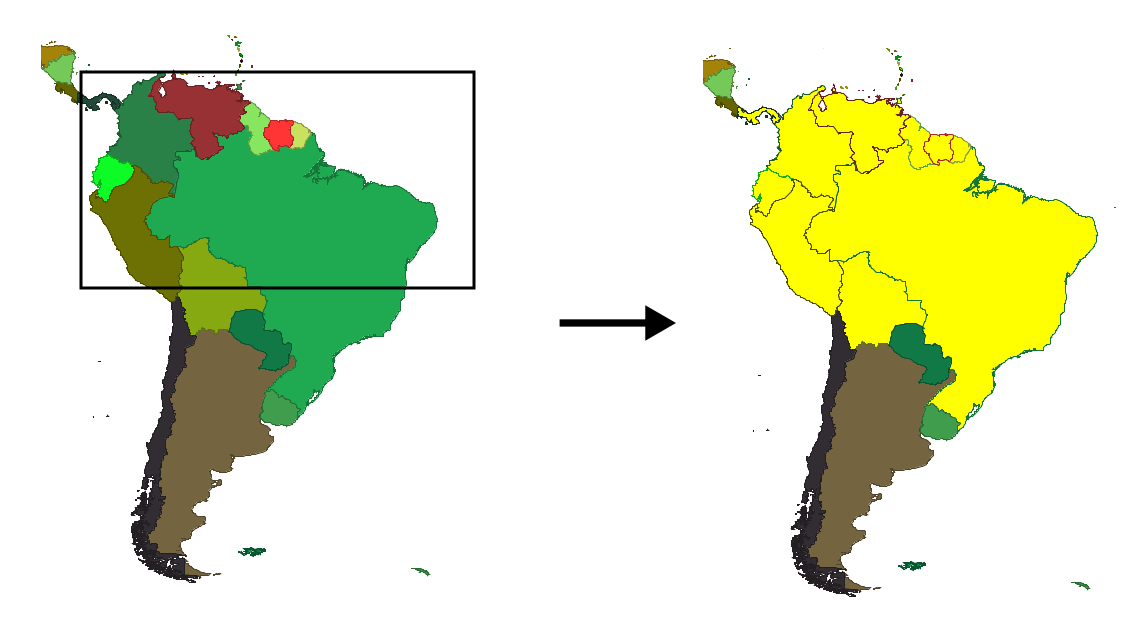
\includegraphics[width=\textwidth]{Bases_dados/Seleccion_rectangulo.png}
\caption{\small Consulta gráfica por seleção. Entidades dentro do retângulo são selecionadas.}
\label{Fig:Seleccion} 
\end{figure}

Exemplos de consultas temáticas:

\begin{itemize}
 \item Países com PIB maior que o do Brasil.
 \item Países com mais de 200 milhões de habitantes.
\end{itemize}

Consultas podem ser combinadas com \textbf{operadores booleanos}:

\begin{itemize}
 \item Países da zona do euro \emph{e} com mais de 40 milhões de habitantes.
 \item Países de língua inglesa \emph{e} com crescimento populacional.
\end{itemize}

Consultas espaciais:

\begin{itemize}
 \item Quais países fazem fronteira com a Argentina?
 \item Quantos países estão inteiramente no hemisfério sul?
 \item Quais países estão a menos de 2000 km do Brasil?
\end{itemize}

Consultas espacio-temáticas:

\begin{itemize}
 \item Países do hemisfério norte com densidade populacional maior que a do Peru.
 \item Países com mais de 10 milhões de habitantes a menos de 1000 km da Rússia.
\end{itemize}

Consultas entre \textbf{múltiplas camadas} também são possíveis. Exemplo: unir cidades com os países onde estão localizadas (por nome ou por localização espacial — \textbf{junção espacial}).

\subsection{Índices espaciais}

Consultas diretas exigem varrer toda a base — o que é ineficiente.

\textbf{Índices} permitem localizar registros rapidamente, sem precisar varrer tudo.

\textbf{Índices espaciais} funcionam de forma semelhante. Eles ajudam o SIG a identificar onde buscar, reduzindo operações desnecessárias.

Exemplo: para saber quais países estão a menos de 3000 km da Espanha, descartamos automaticamente as Américas. Isso é uma forma intuitiva de índice espacial.

O SGBD pode armazenar esses índices junto com os dados ou em arquivos adicionais.

\pagestyle{empty}

  %  \chapter{Análise espacial: Fundamentos}

\pagestyle{fancy}

A análise espacial é uma das tarefas fundamentais, sem a qual o conceito de SIG não atinge seu verdadeiro potencial.

A análise espacial é o \textbf{estudo quantitativo dos fenômenos que se manifestam no espaço}. Isso envolve aspectos cruciais como posição, área, distância e interação espacial.

Fora de um SIG, exemplos de análise espacial incluem: localizar o pico mais alto em um mapa, verificar a altitude de uma cidade, ou planejar uma rota turística considerando distância, tempo e melhores estradas. Todas essas ações são exemplos de análise geográfica — que também podem ser feitas em um SIG.

Através da análise, podemos gerar novos dados como \textbf{camadas geográficas, tabelas, valores escalares} ou \textbf{vetores}.

Às vezes o resultado expressa \textbf{a mesma variável} dos dados de origem (como a média), outras vezes, \textbf{a variável de entrada e saída são diferentes} (por exemplo, gerar uma camada de declividade a partir de uma de elevação).

A análise espacial pode combinar \textbf{diferentes tipos de dados}, como elevação + localização urbana = média de altitude da cidade. Em SIG, seriam duas camadas combinadas no processo.

A análise em SIG permite formular e responder a questões como:

\begin{itemize}
 \item Relacionadas à \textbf{posição e extensão}
 \item Relacionadas à \textbf{forma e distribuição}
 \item Relacionadas à \textbf{associação espacial}
 \item Relacionadas à \textbf{interação espacial}
 \item Relacionadas à \textbf{variação espacial}
\end{itemize}

\section{Exemplos de análise espacial}

\subsection{Consulta espacial}

Consultas, já vistas no capítulo de bancos de dados, podem ser integradas a outras análises — como seleção prévia de entidades a serem analisadas.

\subsection{Análise topológica}

Permite consultas baseadas em \textbf{relações entre elementos}, por exemplo:

\begin{itemize}
 \item Qual o caminho mais curto da minha posição até determinado ponto?
 \item Quais estados fazem fronteira com São Paulo?
\end{itemize}

\subsection{Medições}

Com a referência espacial, é possível \textbf{quantificar}:

\begin{itemize}
 \item Distâncias, áreas, perímetros, índices de forma
 \item Declividade, orientação, índices derivados
\end{itemize}

\subsection{Combinação de camadas}

Combinar ou \textbf{sobrepor camadas} é uma das operações mais características dos SIG.

No caso de camadas vetoriais, são comuns operações como \textbf{união, interseção, diferença e recorte}. Ver Figura~\ref{Fig:Interseccion}.

\begin{figure}[!hbt]   
\centering
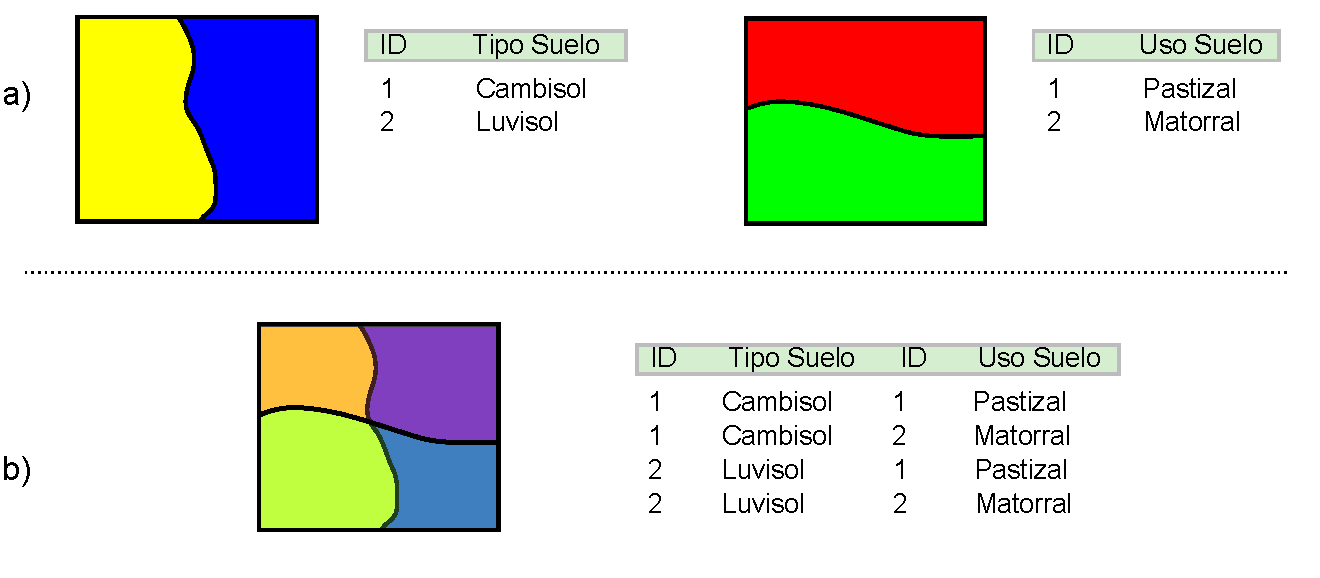
\includegraphics[width= \columnwidth]{Analises/Interseccion.pdf}
\caption{\small Interseção de duas camadas de polígonos.}
\label{Fig:Interseccion} 
\end{figure}

\subsection{Transformações}

Incluem processos como:

\begin{itemize}
 \item \textbf{Transformação de coordenadas}
 \item \textbf{Simplificação de geometria}
 \item \textbf{Áreas de influência}
 \item \textbf{Reclassificação de valores}
 \item \textbf{Conversão entre modelos raster e vetorial}
\end{itemize}

Ver Figura~\ref{Fig:Conversiones} para exemplo de conversão de curvas de nível (vetorial) para MDE (raster).

\begin{figure}[!hbt]   
\centering
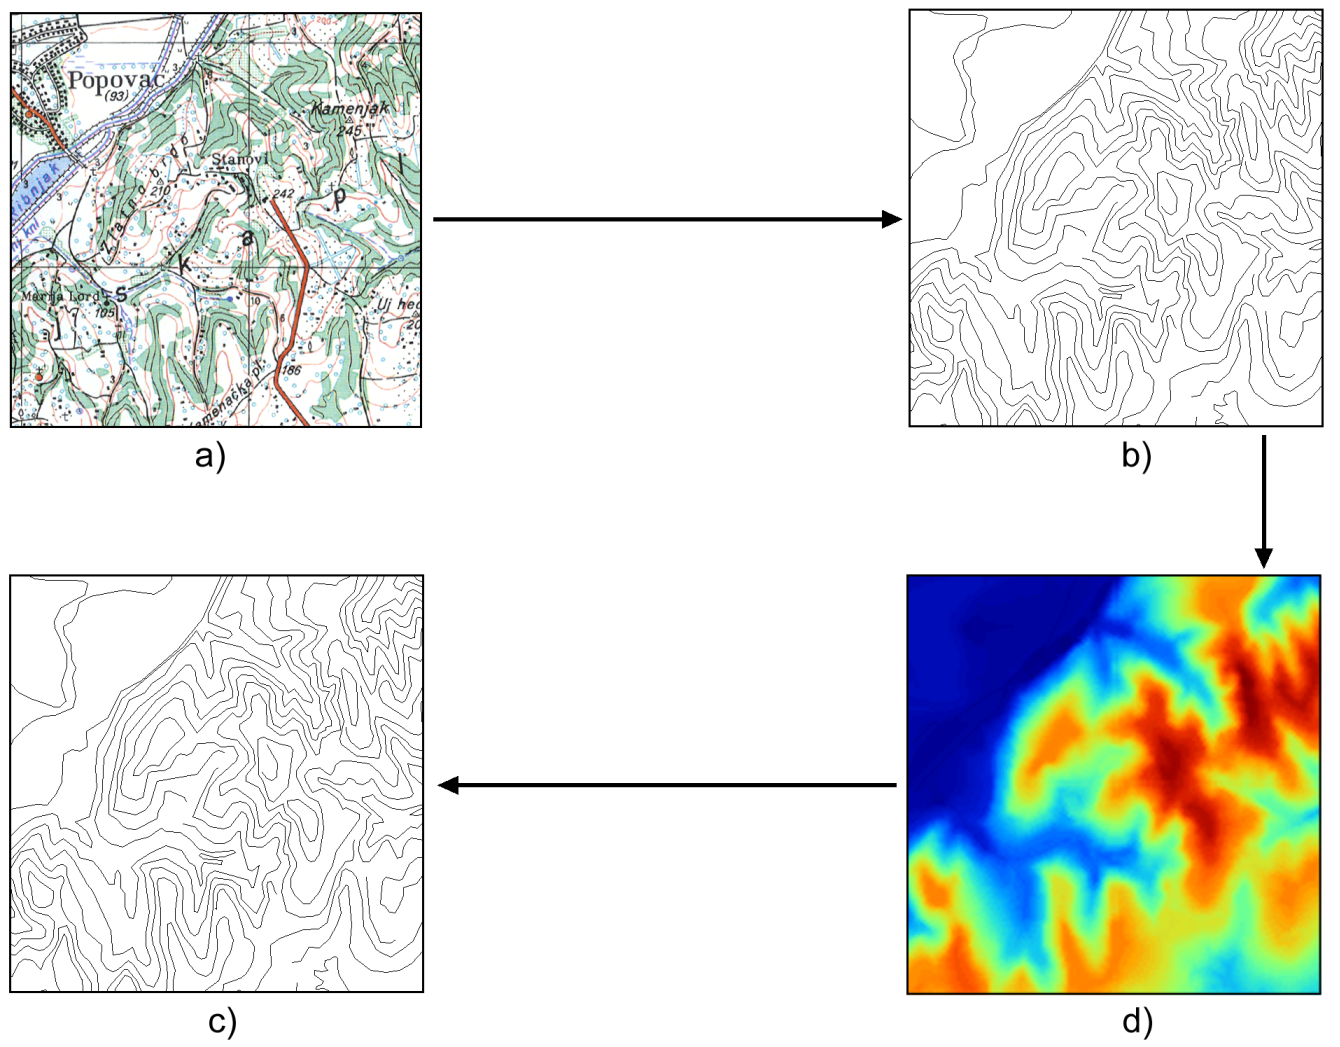
\includegraphics[width= \columnwidth]{Analises/Conversiones.png}
\caption{\small Conversão entre modelos de dados para uma camada de elevação.}
\label{Fig:Conversiones} 
\end{figure}

\subsection{Análise de superfícies}

Inclui:

\begin{itemize}
 \item \textbf{Declividade}, \textbf{orientação}
 \item Análises morfométricas
 \item \textbf{Modelagem hidrológica}
\end{itemize}

\subsection{Estatística descritiva}

Permite avaliar os dados espacialmente com:

\begin{itemize}
 \item Média, mediana, variância
 \item Dependência espacial
 \item Padrões espaciais
\end{itemize}

Exemplos:

\begin{itemize}
 \item A altura média é constante no país?
 \item Há direção predominante nos deslocamentos de uma espécie?
\end{itemize}

\subsection{Inferência}

Utilizada para \textbf{modelar comportamento e prever evolução} espacial ao longo do tempo. Fundamental para análises de mudança e tendência.

\subsection{Tomada de decisão e otimização}

Permite cruzar múltiplos fatores:

\begin{itemize}
 \item Onde construir com menor impacto ambiental?
 \item Onde posicionar um hospital para atender melhor a população?
\end{itemize}

\subsection{Modelagem}

Modelos espaciais são cada vez mais viáveis em SIG — pela estrutura de dados e possibilidade de automação de processos.

\section{Particularidades dos dados espaciais na análise}

\subsection{Escala}

Além da escala cartográfica, existe a \textbf{escala de análise}, que depende dos dados e do tipo de estudo.

Ver Figura~\ref{Fig:Escalas_formas_terreno} — um ponto pode ser uma colina ou fundo de vale dependendo da escala.

\begin{figure}[h]   
\centering
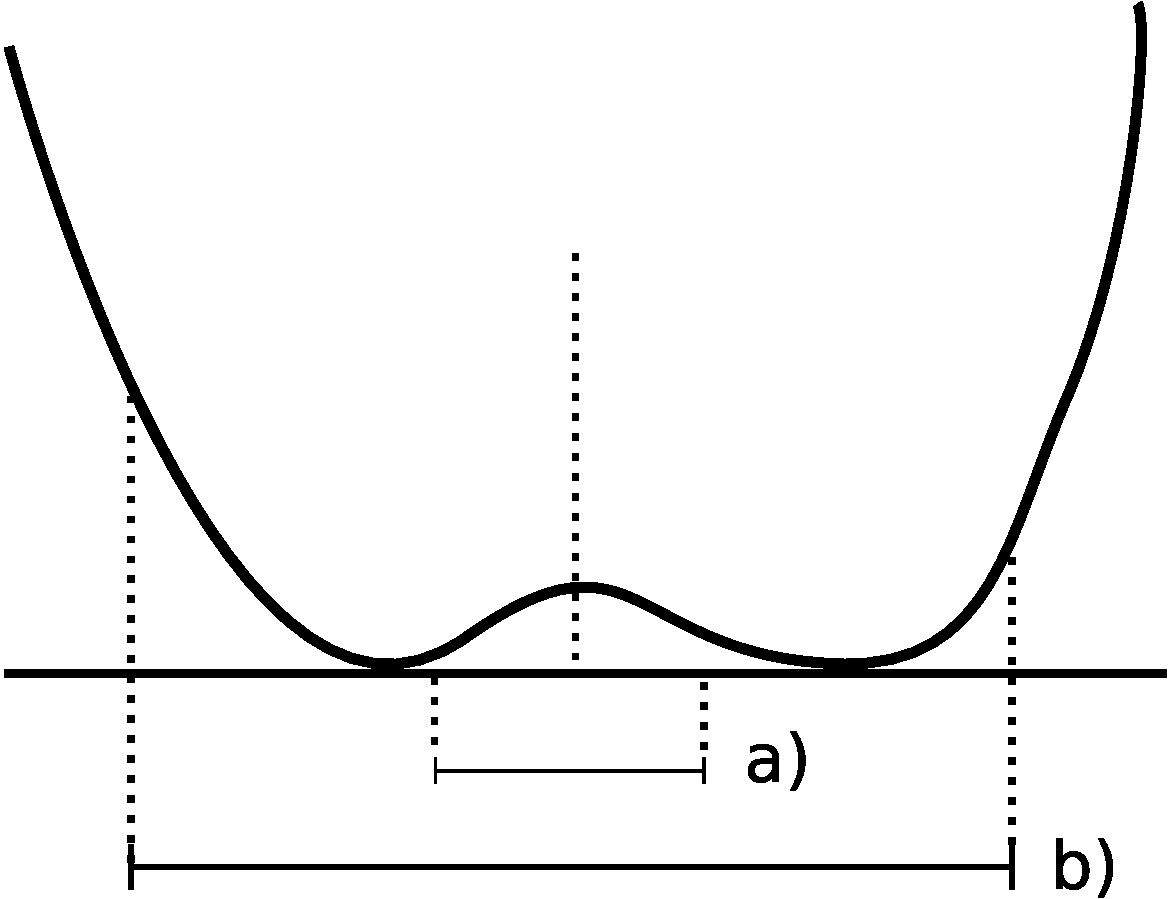
\includegraphics[width= .45\columnwidth]{Analises/Escalas_formas_terreno.pdf}
\caption{\small Um mesmo ponto pode ser identificado como cume (a) ou vale (b), dependendo da escala.}
\label{Fig:Escalas_formas_terreno} 
\end{figure}

Também se aplica à \textbf{medição de comprimentos}, como mostra a Figura~\ref{Fig:Medida_linea_fractal}.

\begin{figure}[h]   
\centering
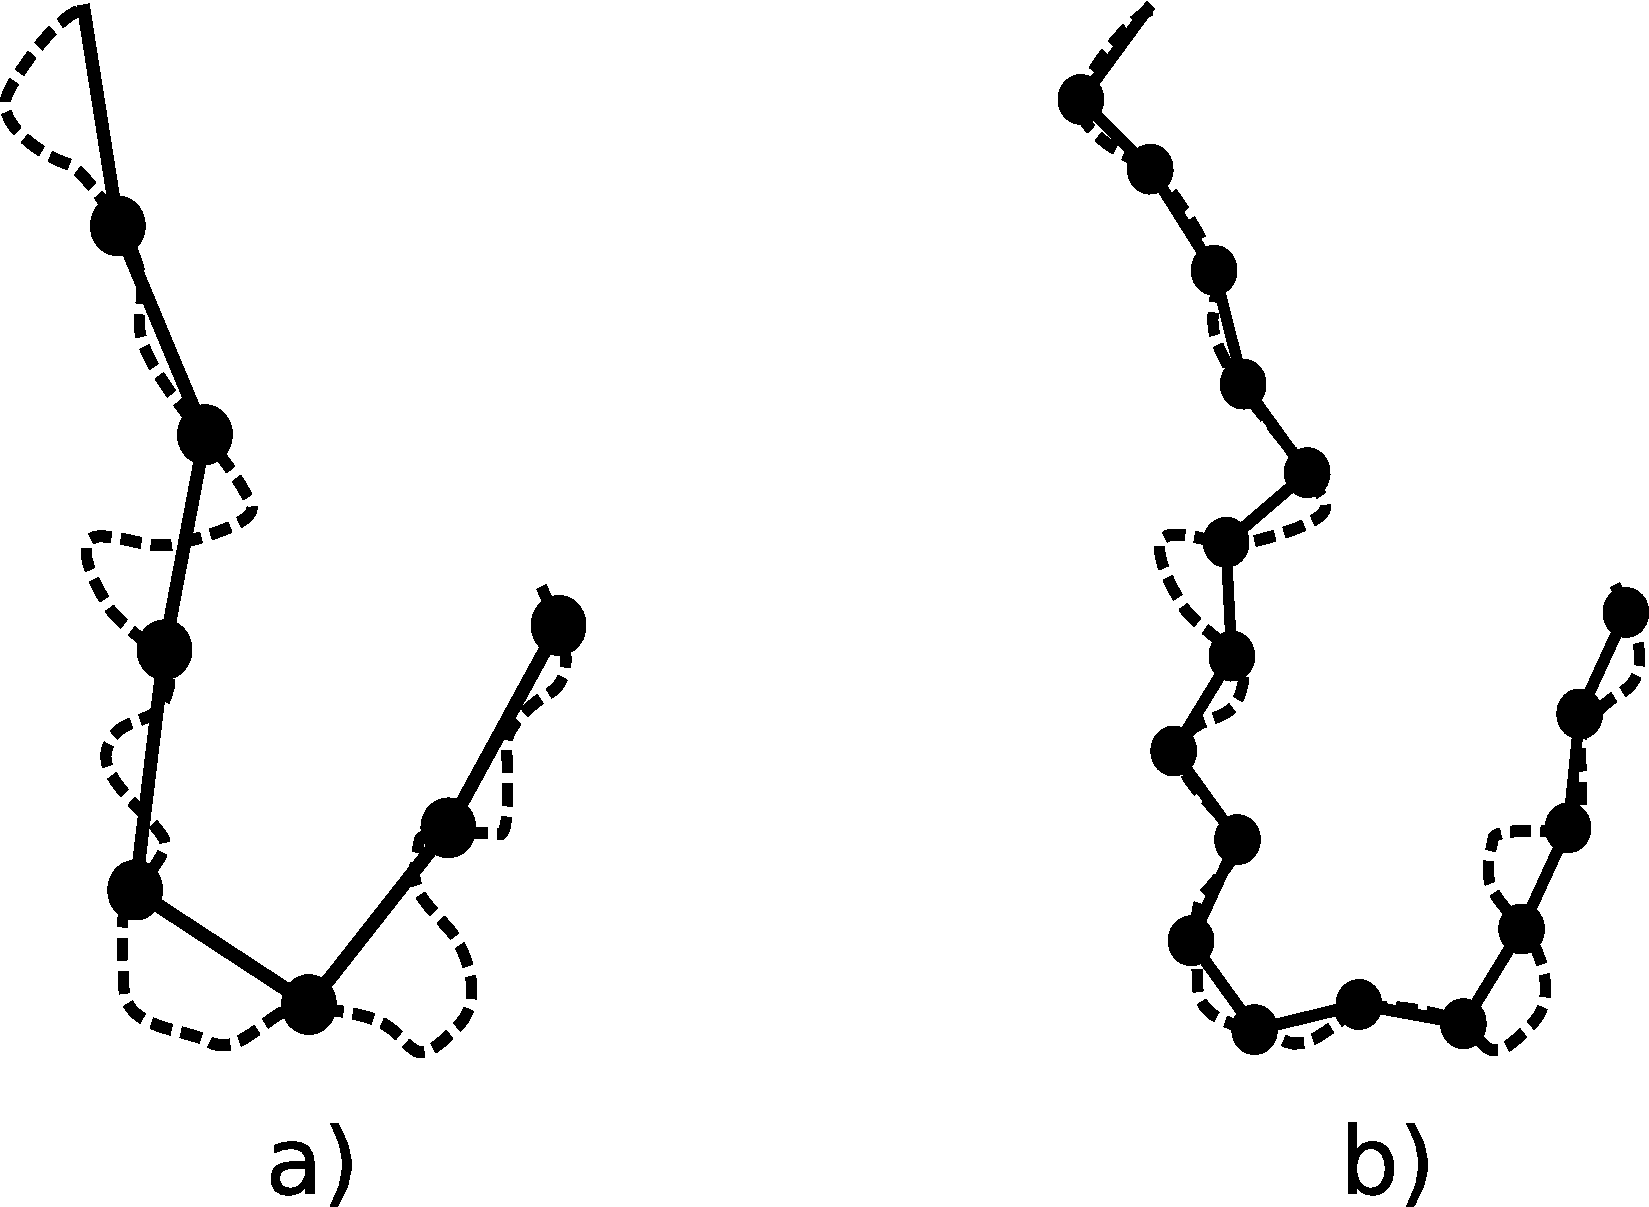
\includegraphics[width= .45\columnwidth]{Analises/Medida_linea_fractal.pdf}
\caption{\small O comprimento medido depende da unidade usada.}
\label{Fig:Medida_linea_fractal} 
\end{figure}

Isso está diretamente ligado ao conceito de \textbf{fractal}.

O \textbf{formato de dados} também limita a escala — ex: \textbf{tamanho da célula} em dados raster.

\subsection{Problema da Unidade de Área Modificável (PUAM)}

Algumas variáveis (ex: densidade populacional) não são pontuais, mas calculadas por área.

As unidades usadas (distritos, municípios) são arbitrárias e \textbf{afetam os resultados}. Isso é o PUAM.

Relacionado a isso, temos a \textbf{falácia ecológica}: assumir que os dados médios de uma área valem para todos os indivíduos nela contidos.

\subsection{Autocorrelação espacial}

É a \textbf{correlação de uma variável consigo mesma no espaço}. Pode ser:

\begin{itemize}
 \item \textbf{Positiva} — valores semelhantes próximos (temperatura)
 \item \textbf{Negativa} — valores opostos próximos
 \item \textbf{Inexistente} — valores independentes no espaço
\end{itemize}

Ver Figura~\ref{Fig:Autocorrelacion_espacial}.

\begin{figure}[!hbt]   
\centering
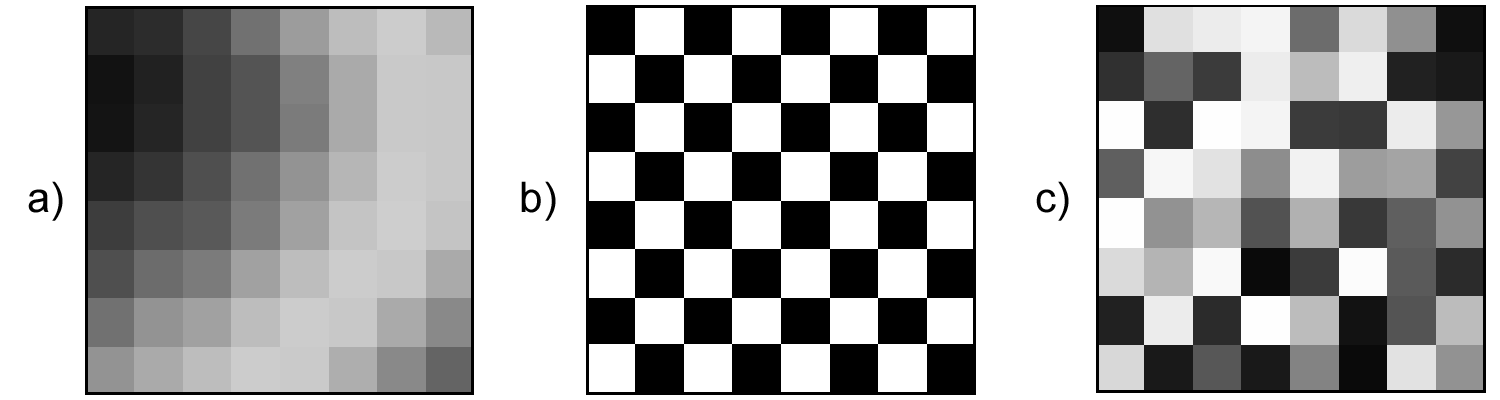
\includegraphics[width=\textwidth]{Analises/Autocorrelacion_espacial.png}
\caption{\small a) Positiva, b) Negativa, c) Sem correlação espacial.}
\label{Fig:Autocorrelacion_espacial} 
\end{figure}

A autocorrelação viola suposições estatísticas de independência. Deve ser considerada nos modelos. Porém, pode ser usada para \textbf{interpolação}.

\subsection{Estrutura dos dados espaciais}

Dois conceitos definem a estrutura espacial:

\begin{itemize}
 \item \textbf{Estacionaridade} — invariância por translação (sem tendência espacial)
 \item \textbf{Isotropia} — invariância por rotação (mesmo comportamento em todas as direções)
\end{itemize}

\subsection{Efeitos de borda}

Limites artificiais ou naturais distorcem análises, especialmente em parâmetros que dependem de área (ex: densidade).

Além disso, o \textbf{efeito pode se propagar} — elementos conectados ao limite também são afetados, mesmo se estiverem longe.

\pagestyle{empty}

  %  \chapter{Visualização e representação de dados espaciais}

\pagestyle{fancy}

Visualizar a informação geográfica é parte fundamental do trabalho com SIG. Embora alguns dados já incluam sua forma própria de representação — como imagens de satélite, ortofotos ou serviços de mapas —, no SIG geralmente é o usuário quem define como o dado será representado. Ou seja, o usuário de SIG \textbf{assume o papel de cartógrafo}, devendo, portanto, conhecer os fundamentos utilizados na criação de mapas.

Além das ferramentas e conceitos clássicos da cartografia, os SIG incorporam elementos da chamada \textbf{visualização científica}, como a \textbf{interatividade} e a \textbf{representação de dados multidimensionais}. Esse novo enfoque, mais rico que o da cartografia tradicional, é conhecido como \textbf{geovisualização}.

Neste capítulo, veremos as ideias fundamentais da visualização de dados, abordando tanto sua aplicação na cartografia tradicional quanto em SIGs e geovisualização.

\section{Conceitos básicos de visualização}

Sempre que visualizamos informação geográfica — em um mapa impresso ou em uma tela de computador — utilizamos uma forma de \textbf{linguagem visual}.

O estudo dos signos de uma linguagem é chamado de \textbf{semiologia}. Quando aplicada à linguagem visual, temos a \textbf{semiologia gráfica}, que define uma gramática visual para compreender como os elementos gráficos transmitem a informação desejada.

\subsection{As variáveis visuais}

Existem diferentes propriedades dos elementos visuais que podemos usar para comunicar informação. Cada uma é mais ou menos adequada dependendo do tipo de dado representado.

\begin{figure}[!hbt]
\centering
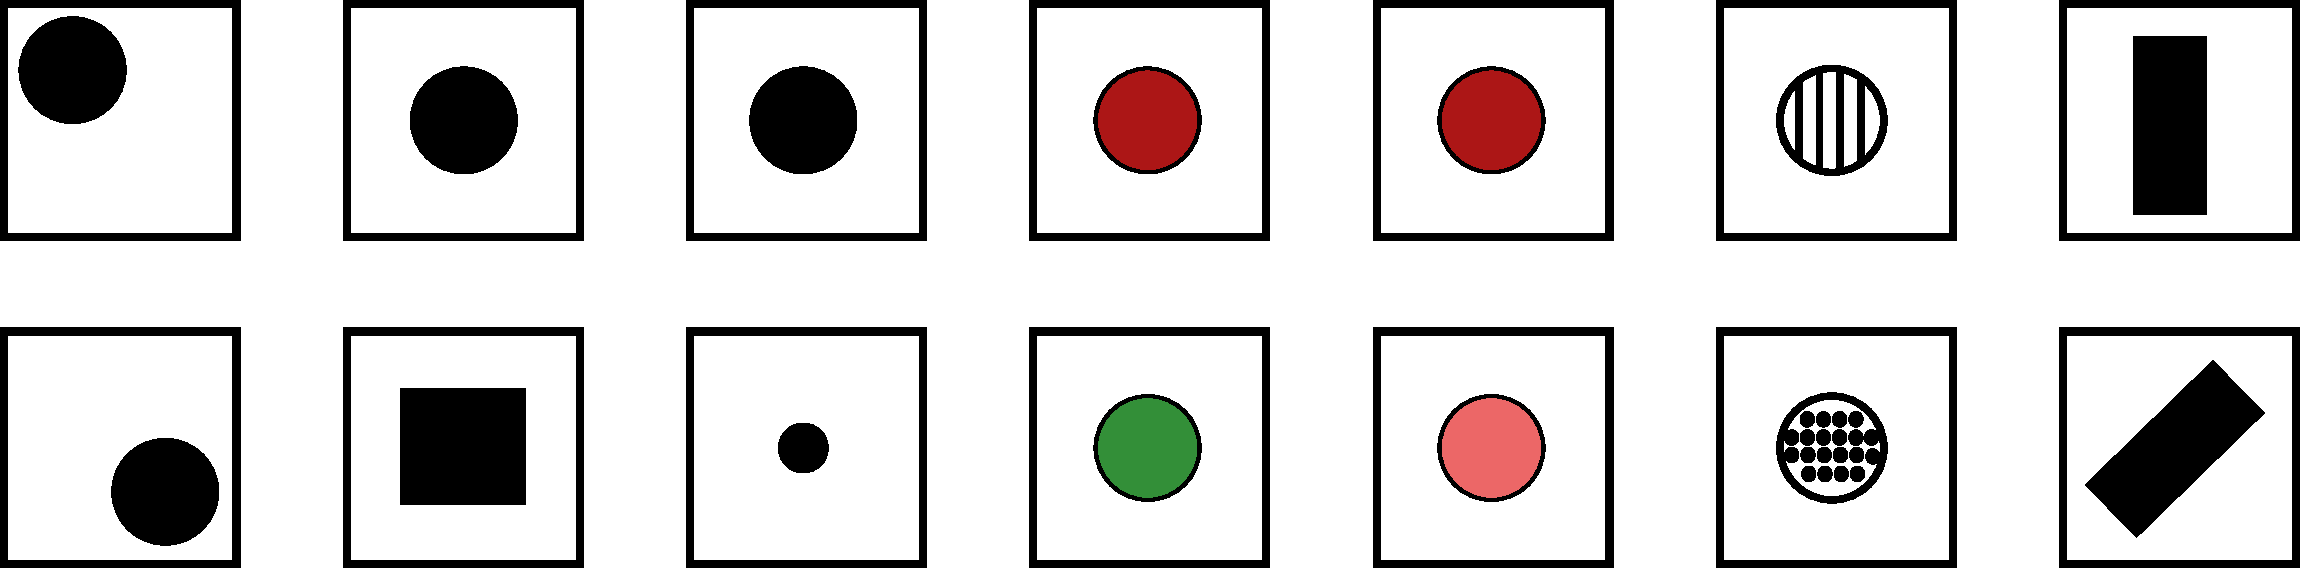
\includegraphics[width=\columnwidth]{Visualizacao/VariablesVisuales.pdf}
\caption{\small Exemplos de uso das variáveis visuais: posição, forma, tamanho, tom, valor, textura e orientação.}
\label{Fig:VariablesVisuales} 
\end{figure}

Essas propriedades são chamadas de \textbf{variáveis visuais}. Elas se aplicam aos elementos geométricos básicos da representação. São: posição, forma, tamanho, textura, cor e orientação (Figura~\ref{Fig:VariablesVisuales}).

- A \textbf{posição} não é livre em mapas, pois deve respeitar a localização geográfica real.
- A \textbf{forma} refere-se ao contorno dos símbolos, especialmente em pontos. Seu uso em linhas e polígonos é limitado.
- O \textbf{tamanho} aplica-se diretamente em pontos (maior símbolo = maior valor) e linhas (espessura). Para polígonos, aplica-se mais à textura.
- A \textbf{textura} envolve padrões internos nos símbolos, como hachuras.
- A \textbf{cor} é a variável visual mais poderosa. Divide-se em:
  - \textbf{Tom}: nome da cor (ex: vermelho, azul)
  - \textbf{Valor}: claridade ou escuridão da cor
- A \textbf{orientação} altera o ângulo de símbolos ou padrões.

\subsection{Propriedades das variáveis visuais}

Cada variável visual pode ter uma ou mais destas 4 propriedades:

\begin{itemize}
	\item \textbf{Associativa}: não altera o destaque de um símbolo
	\item \textbf{Seletiva}: permite categorizar os símbolos
	\item \textbf{Ordenada}: transmite uma ordem ou sequência
	\item \textbf{Quantitativa}: expressa proporções ou quantidades
\end{itemize}

Essas propriedades estão organizadas em \emph{níveis de organização}. A Tabela~\ref{Tabla:PropiedadesVariablesVisuales} resume como cada variável se comporta:

\begin{table}[!hbt]
\small
\centering  \label{Tabla:PropiedadesVariablesVisuales}
\begin{tabular}{p{3.6cm}ccccccc}  
 & \rotatebox{90}{\textbf{Posição}} & \rotatebox{90}{\textbf{Tamanho}} & \rotatebox{90}{\textbf{Forma}} & \rotatebox{90}{\textbf{Valor}} & \rotatebox{90}{\textbf{Tom}} & \rotatebox{90}{\textbf{Textura}} & \rotatebox{90}{\textbf{Orientação}} \\ \midrule   
\textbf{Associativa} & $\diamondsuit$ & - & $\diamondsuit$ & - & $\diamondsuit$ & $\diamondsuit$ & $\diamondsuit$ \\
\textbf{Seletiva}   & $\diamondsuit$ & $\diamondsuit$ & - & $\diamondsuit$ & $\diamondsuit$ & $\diamondsuit$ & $\diamondsuit$ \\
\textbf{Ordenada}   & $\diamondsuit$ & $\diamondsuit$ & - & $\diamondsuit$ & - & - & - \\
\textbf{Quantitativa} & $\diamondsuit$ & $\diamondsuit$ & - & - & - & - & -  \\
\bottomrule \end{tabular}
\caption{\small Resumo das propriedades das variáveis visuais.}
\end{table}

\subsection{Percepção das variáveis visuais}

A percepção de uma variável visual pode ser afetada pelo \textbf{contexto visual} — como cor de fundo, contraste com vizinhos, entre outros.

Conceitos importantes:

- \textbf{Constância perceptiva}: percebemos um objeto como o mesmo, mesmo sob mudanças (ex: forma circular vista em perspectiva).
- \textbf{Contraste perceptivo}: a percepção muda mesmo que o objeto não tenha mudado.

Recomendações para minimizar erros de percepção:

- Evitar sobreposição de tamanhos diferentes
- Cuidar do contraste de valor e tom
- Usar cores com cuidado para evitar ilusões visuais (ex: vibração entre complementares)
- Estabelecer uma \textbf{hierarquia visual} clara entre elementos (Figura~\ref{Fig:JerarquiaMapa})

\begin{figure}[!hbt]
\centering
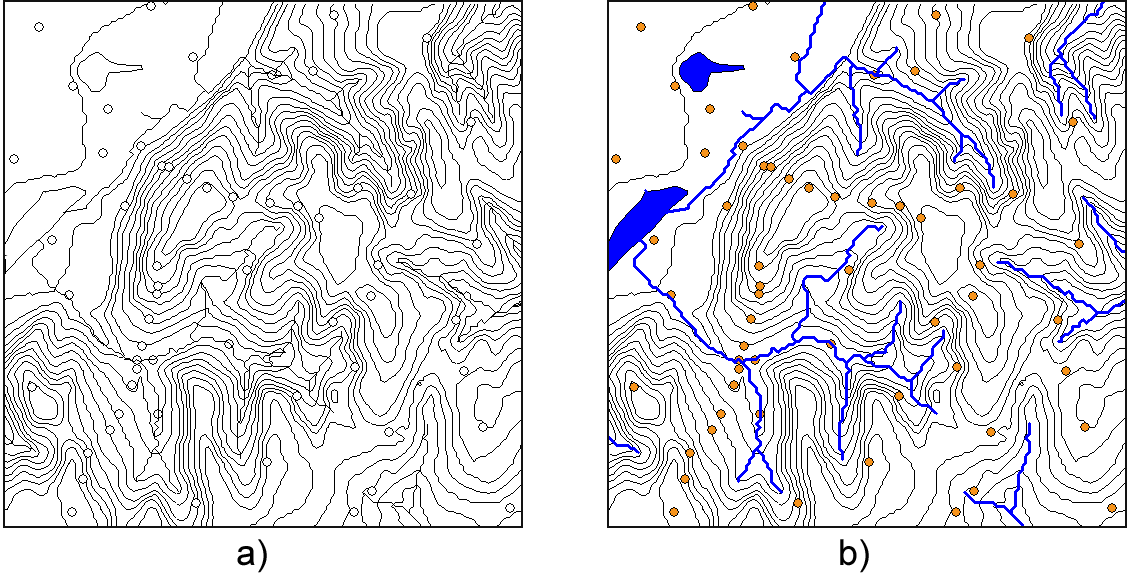
\includegraphics[width=\columnwidth]{Visualizacao/JerarquiaMapa.png}
\caption{\small Mapa com hierarquia incorreta (a) e correta (b).}
\label{Fig:JerarquiaMapa} 
\end{figure}

\section{Mapas e comunicação cartográfica}

Mapas são formas visuais de comunicar relações espaciais. São abstrações simbólicas e generalizadas da realidade.

Dois tipos principais:

\begin{itemize}
 \item \textbf{Cartografia base (topográfica)}: descreve o terreno físico
 \item \textbf{Cartografia temática}: representa uma variável específica (social, política, ambiental etc.)
\end{itemize}

Cartografia temática costuma se apoiar na cartografia base.

\subsection{Tipos de informação e representação}

Escolher a variável visual correta depende do tipo de dado:

\begin{itemize}
 \item \textbf{Nominal}: usar forma, tom ou textura
 \item \textbf{Ordinal}: requer variável com propriedade \emph{ordenada}
 \item \textbf{Intervalar e razão}: preferir \emph{tamanho}, que tem a propriedade \emph{quantitativa}
\end{itemize}

É comum agrupar valores contínuos em classes: intervalos iguais, percentis, intervalos naturais, etc. (ver Figura~\ref{Fig:TiposIntervalosClases})

\begin{figure}[!hbt]
\centering
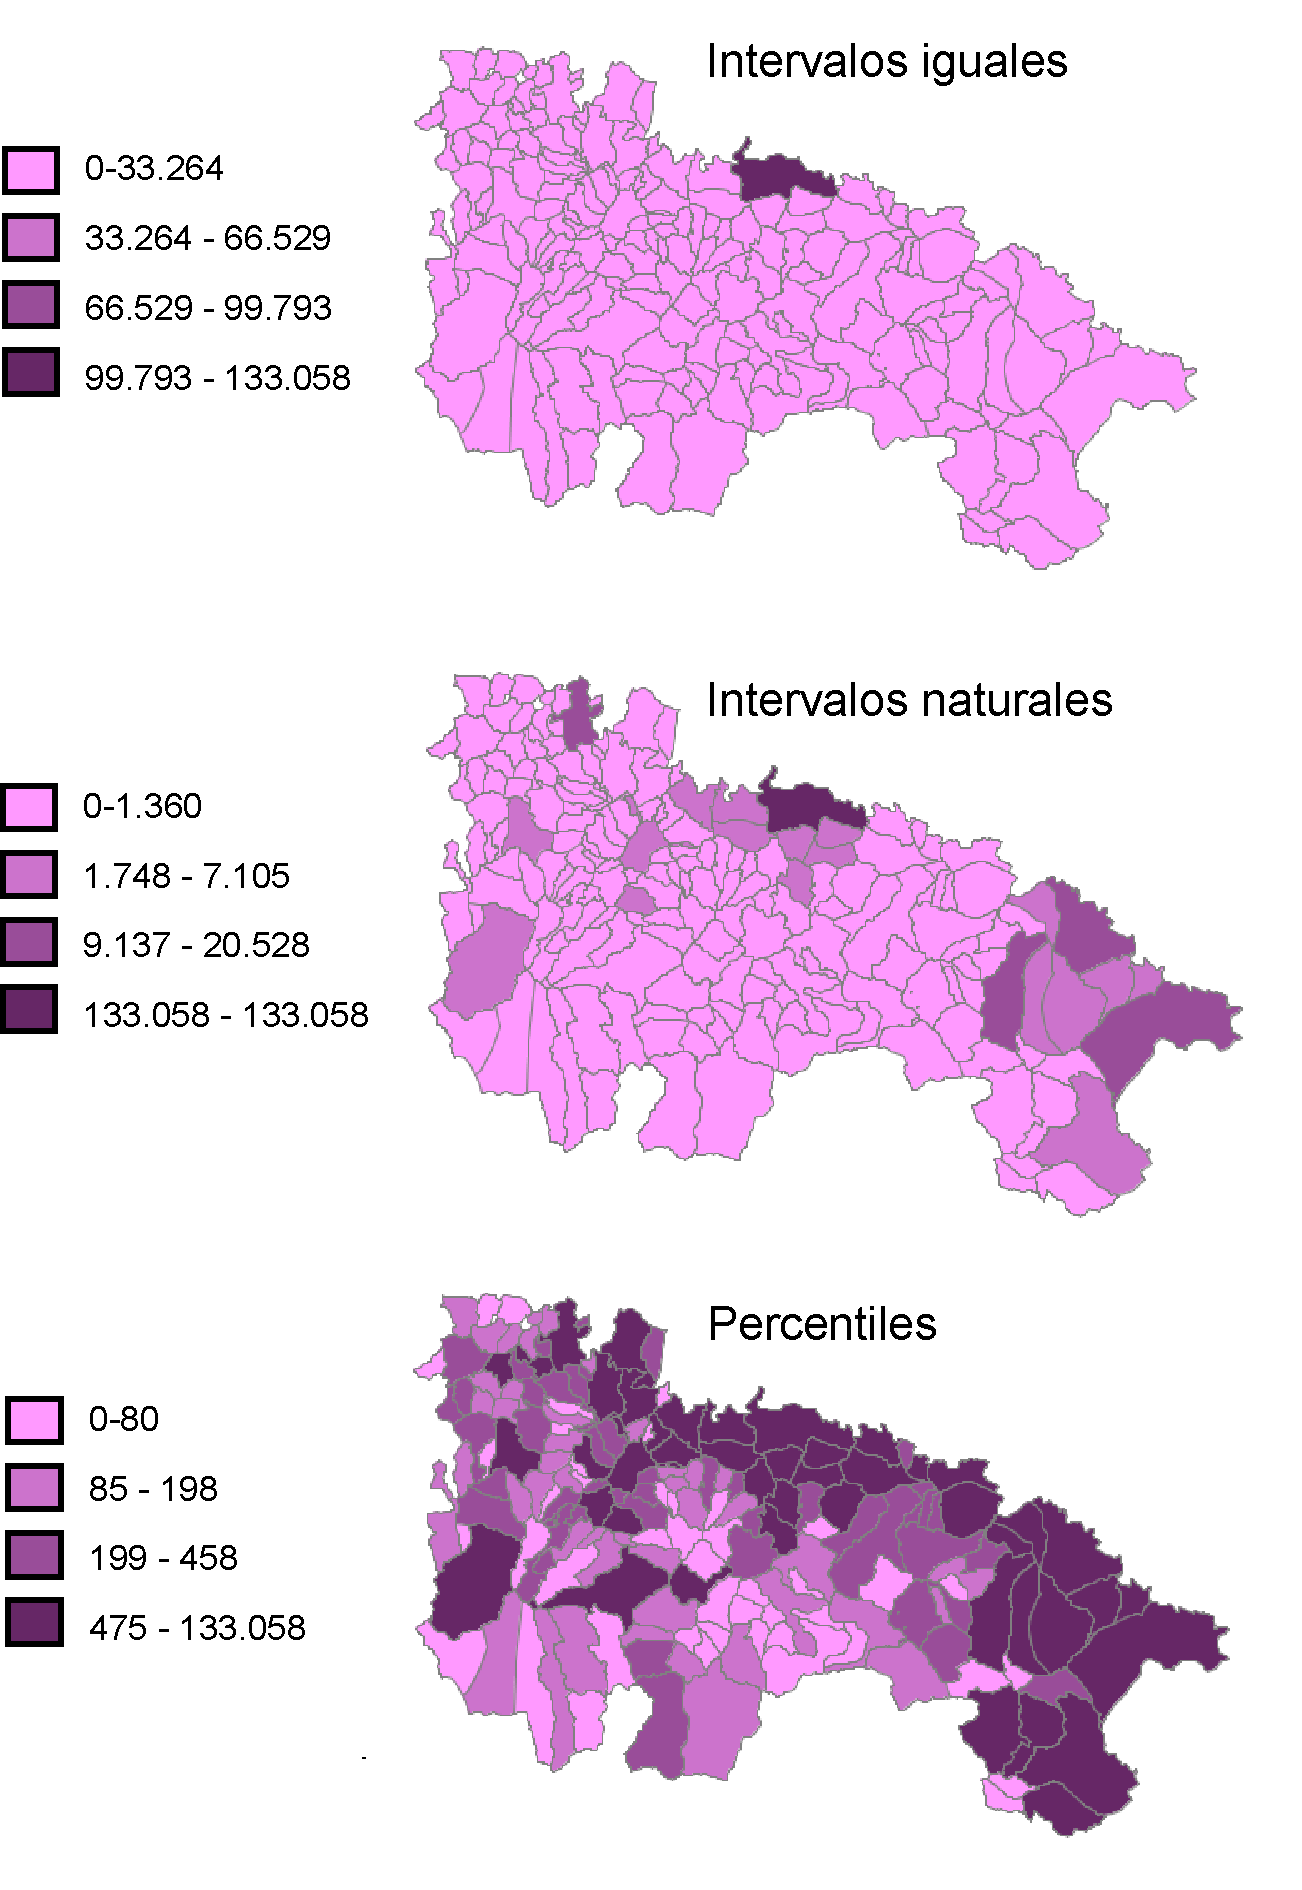
\includegraphics[width=.7\columnwidth]{Visualizacao/TiposIntervalosClases.pdf}
\caption{\small Diferenças entre métodos de classificação em mapas.}
\label{Fig:TiposIntervalosClases} 
\end{figure}

\subsection{Elementos do mapa}

Elementos comuns em mapas (Figura~\ref{Fig:ElementosMapa}):

\begin{figure}[!hbt]
\centering
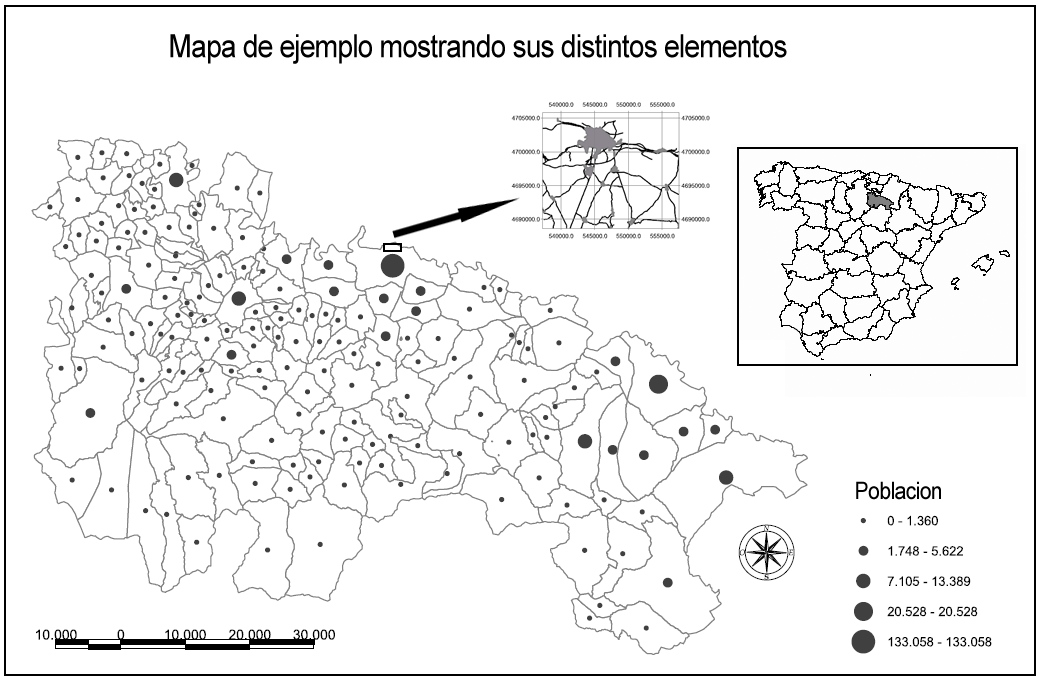
\includegraphics[width=\columnwidth]{Visualizacao/ElementosMapa.png}
\caption{\small Elementos principais de um mapa.}
\label{Fig:ElementosMapa} 
\end{figure}

\begin{itemize}
 \item Título
 \item Autor
 \item Informações complementares (ex: sistema de referência)
 \item Canevás (grade)
 \item Legenda
 \item Norte
 \item Escala (gráfica e numérica)
 \item Mapa de localização (contexto geográfico)
 \item Mapa de detalhe (zoom em áreas específicas)
\end{itemize}

\section{Tipos de mapas temáticos}

Apresentamos aqui os quatro principais tipos para variáveis quantitativas:

\subsection{Símbolos proporcionais}

Tamanho do símbolo proporcional ao valor representado.

Importante:

- Usar escalonamento discreto (classes)
- Incluir legenda clara (Figura~\ref{Fig:EjemplosLeyendaSimbolosProporcionales})

\begin{figure}[!hbt]
\centering
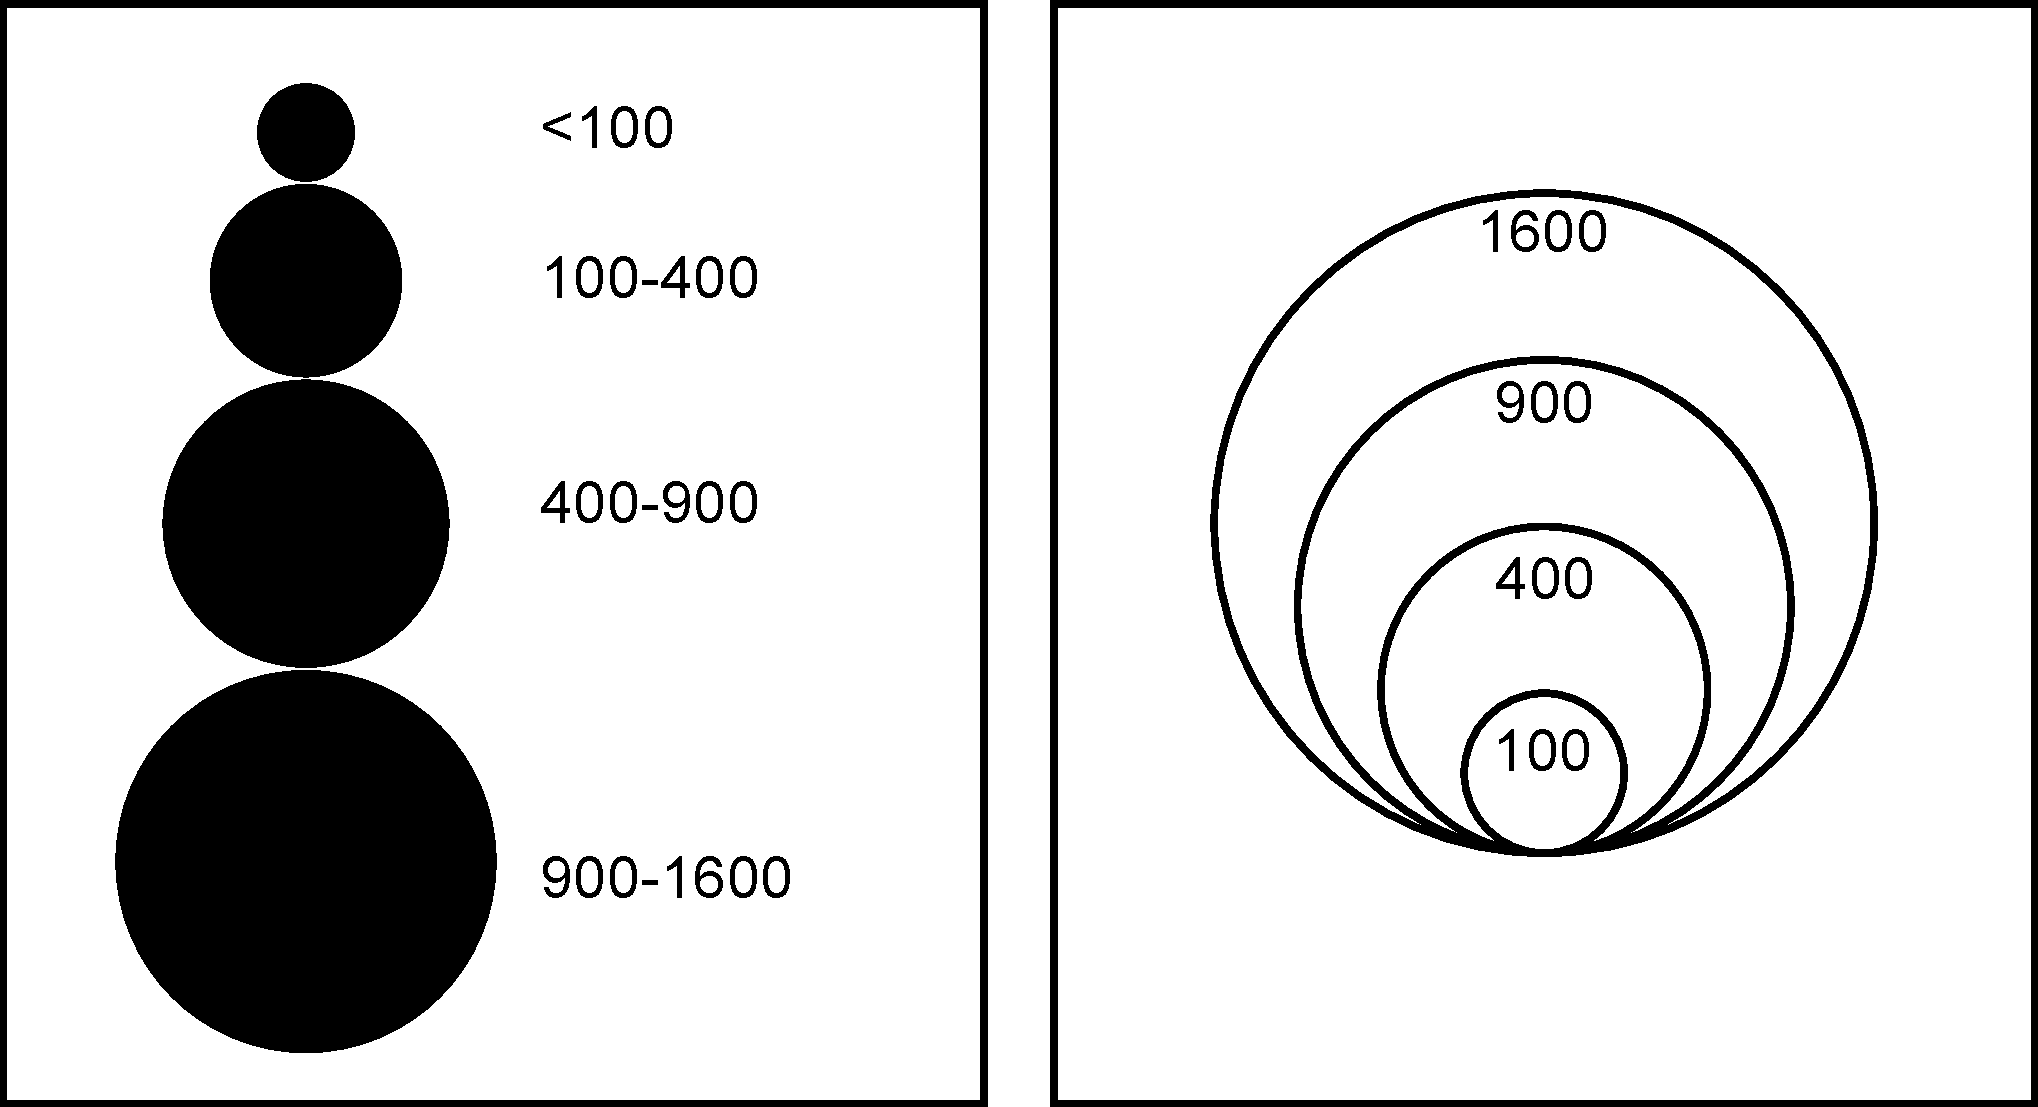
\includegraphics[width=.65\columnwidth]{Visualizacao/EjemplosLeyendaSimbolosProporcionales.pdf}
\caption{\small Exemplos de legendas para símbolos proporcionais.}
\label{Fig:EjemplosLeyendaSimbolosProporcionales} 
\end{figure}

\subsection{Mapas de pontos}

Usados para variáveis como população ou produção agrícola.

Aspectos importantes:

- Valor unitário por ponto
- Tamanho visível e adequado
- Posição coerente com distribuição esperada (Figura~\ref{Fig:MapaPontos})

\begin{figure}[!hbt]
\centering
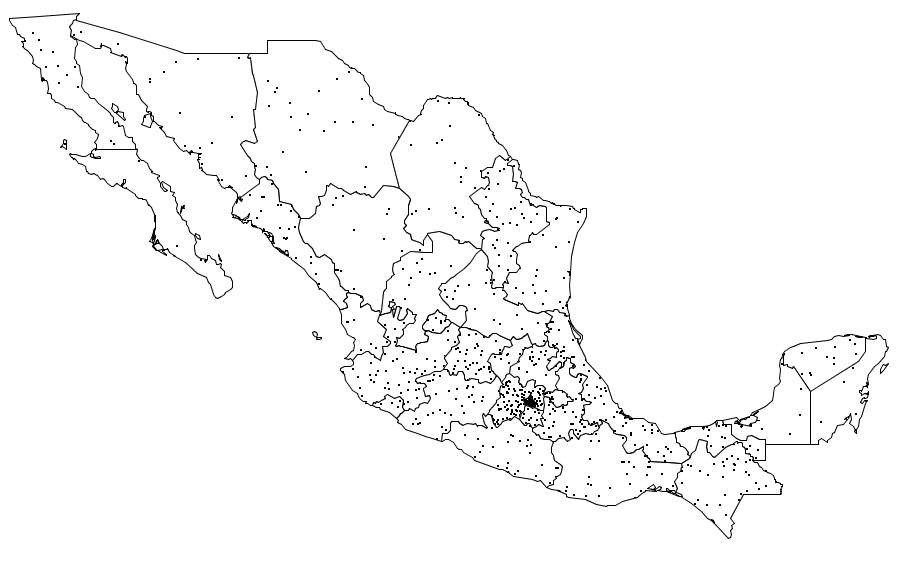
\includegraphics[width=.8\columnwidth]{Visualizacao/MapaPuntos.png}
\caption{\small Exemplo de mapa de pontos.}
\label{Fig:MapaPontos} 
\end{figure}

\subsection{Mapas de isolinhas}

Representam variáveis contínuas, como altitude ou temperatura.

- Linhas conectam pontos de mesmo valor
- \emph{Equidistância} define o espaçamento entre linhas
- Variável visual usada: espessura (para linhas principais)
- Pode-se usar coloração entre as linhas: \emph{isocoropletas} (Figura~\ref{Fig:Isolineas})

\begin{figure}[!hbt]
\centering
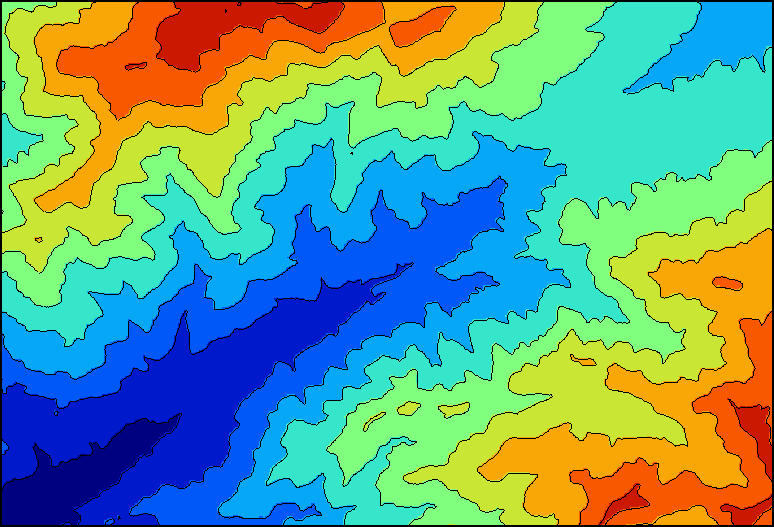
\includegraphics[width=.8\columnwidth]{Visualizacao/Isolineas.png}
\caption{\small Mapa com isolinhas e preenchimento por classes.}
\label{Fig:Isolineas} 
\end{figure}

\subsection{Mapas de coropléticas}

Usados para dados agregados por áreas.

- Representam o valor da variável por meio da cor
- Devem normalizar por área (ex: densidade populacional)
- Podem induzir interpretação errada: mudança brusca nos limites; homogeneidade interna

\section{Visualização em SIG}

Dois aspectos fundamentais:

\begin{itemize}
 \item \textbf{Composição de múltiplas camadas}
 \item \textbf{Particularidades da tela e da interatividade}
\end{itemize}

\subsection{Composição de camadas}

Importante para enriquecer a interpretação.

Boas práticas:

- Definir a \textbf{ordem de desenho}: ráster abaixo de vetores; polígonos abaixo de linhas e pontos
- Usar \textbf{transparência} quando necessário (Figura~\ref{Fig:CombinacionCapas})

\begin{figure}[!hbt]
\centering
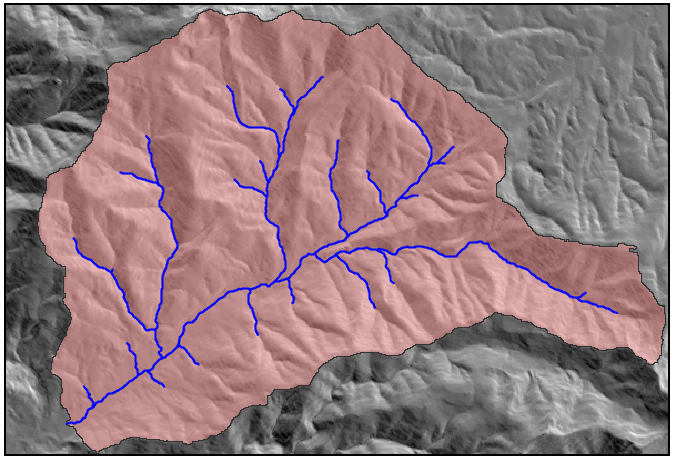
\includegraphics[width=.7\columnwidth]{Visualizacao/CombinacionCapas.png}
\caption{\small Uso de transparência para visualizar camadas sobrepostas.}
\label{Fig:CombinacionCapas} 
\end{figure}

\subsection{Particularidades da tela}

Duas limitações:

\begin{itemize}
 \item \textbf{Baixa resolução}: evitar fontes com ornamentos ou linhas muito finas
 \item \textbf{Interatividade}: o usuário pode mudar a escala (zoom)
\end{itemize}

Problemas comuns:

- Símbolos ficam ilegíveis em escalas pequenas ou exagerados em escalas grandes (Figura~\ref{Fig:ProblemasRepresentacionSimbolos})

\begin{figure}[!hbt]
\centering
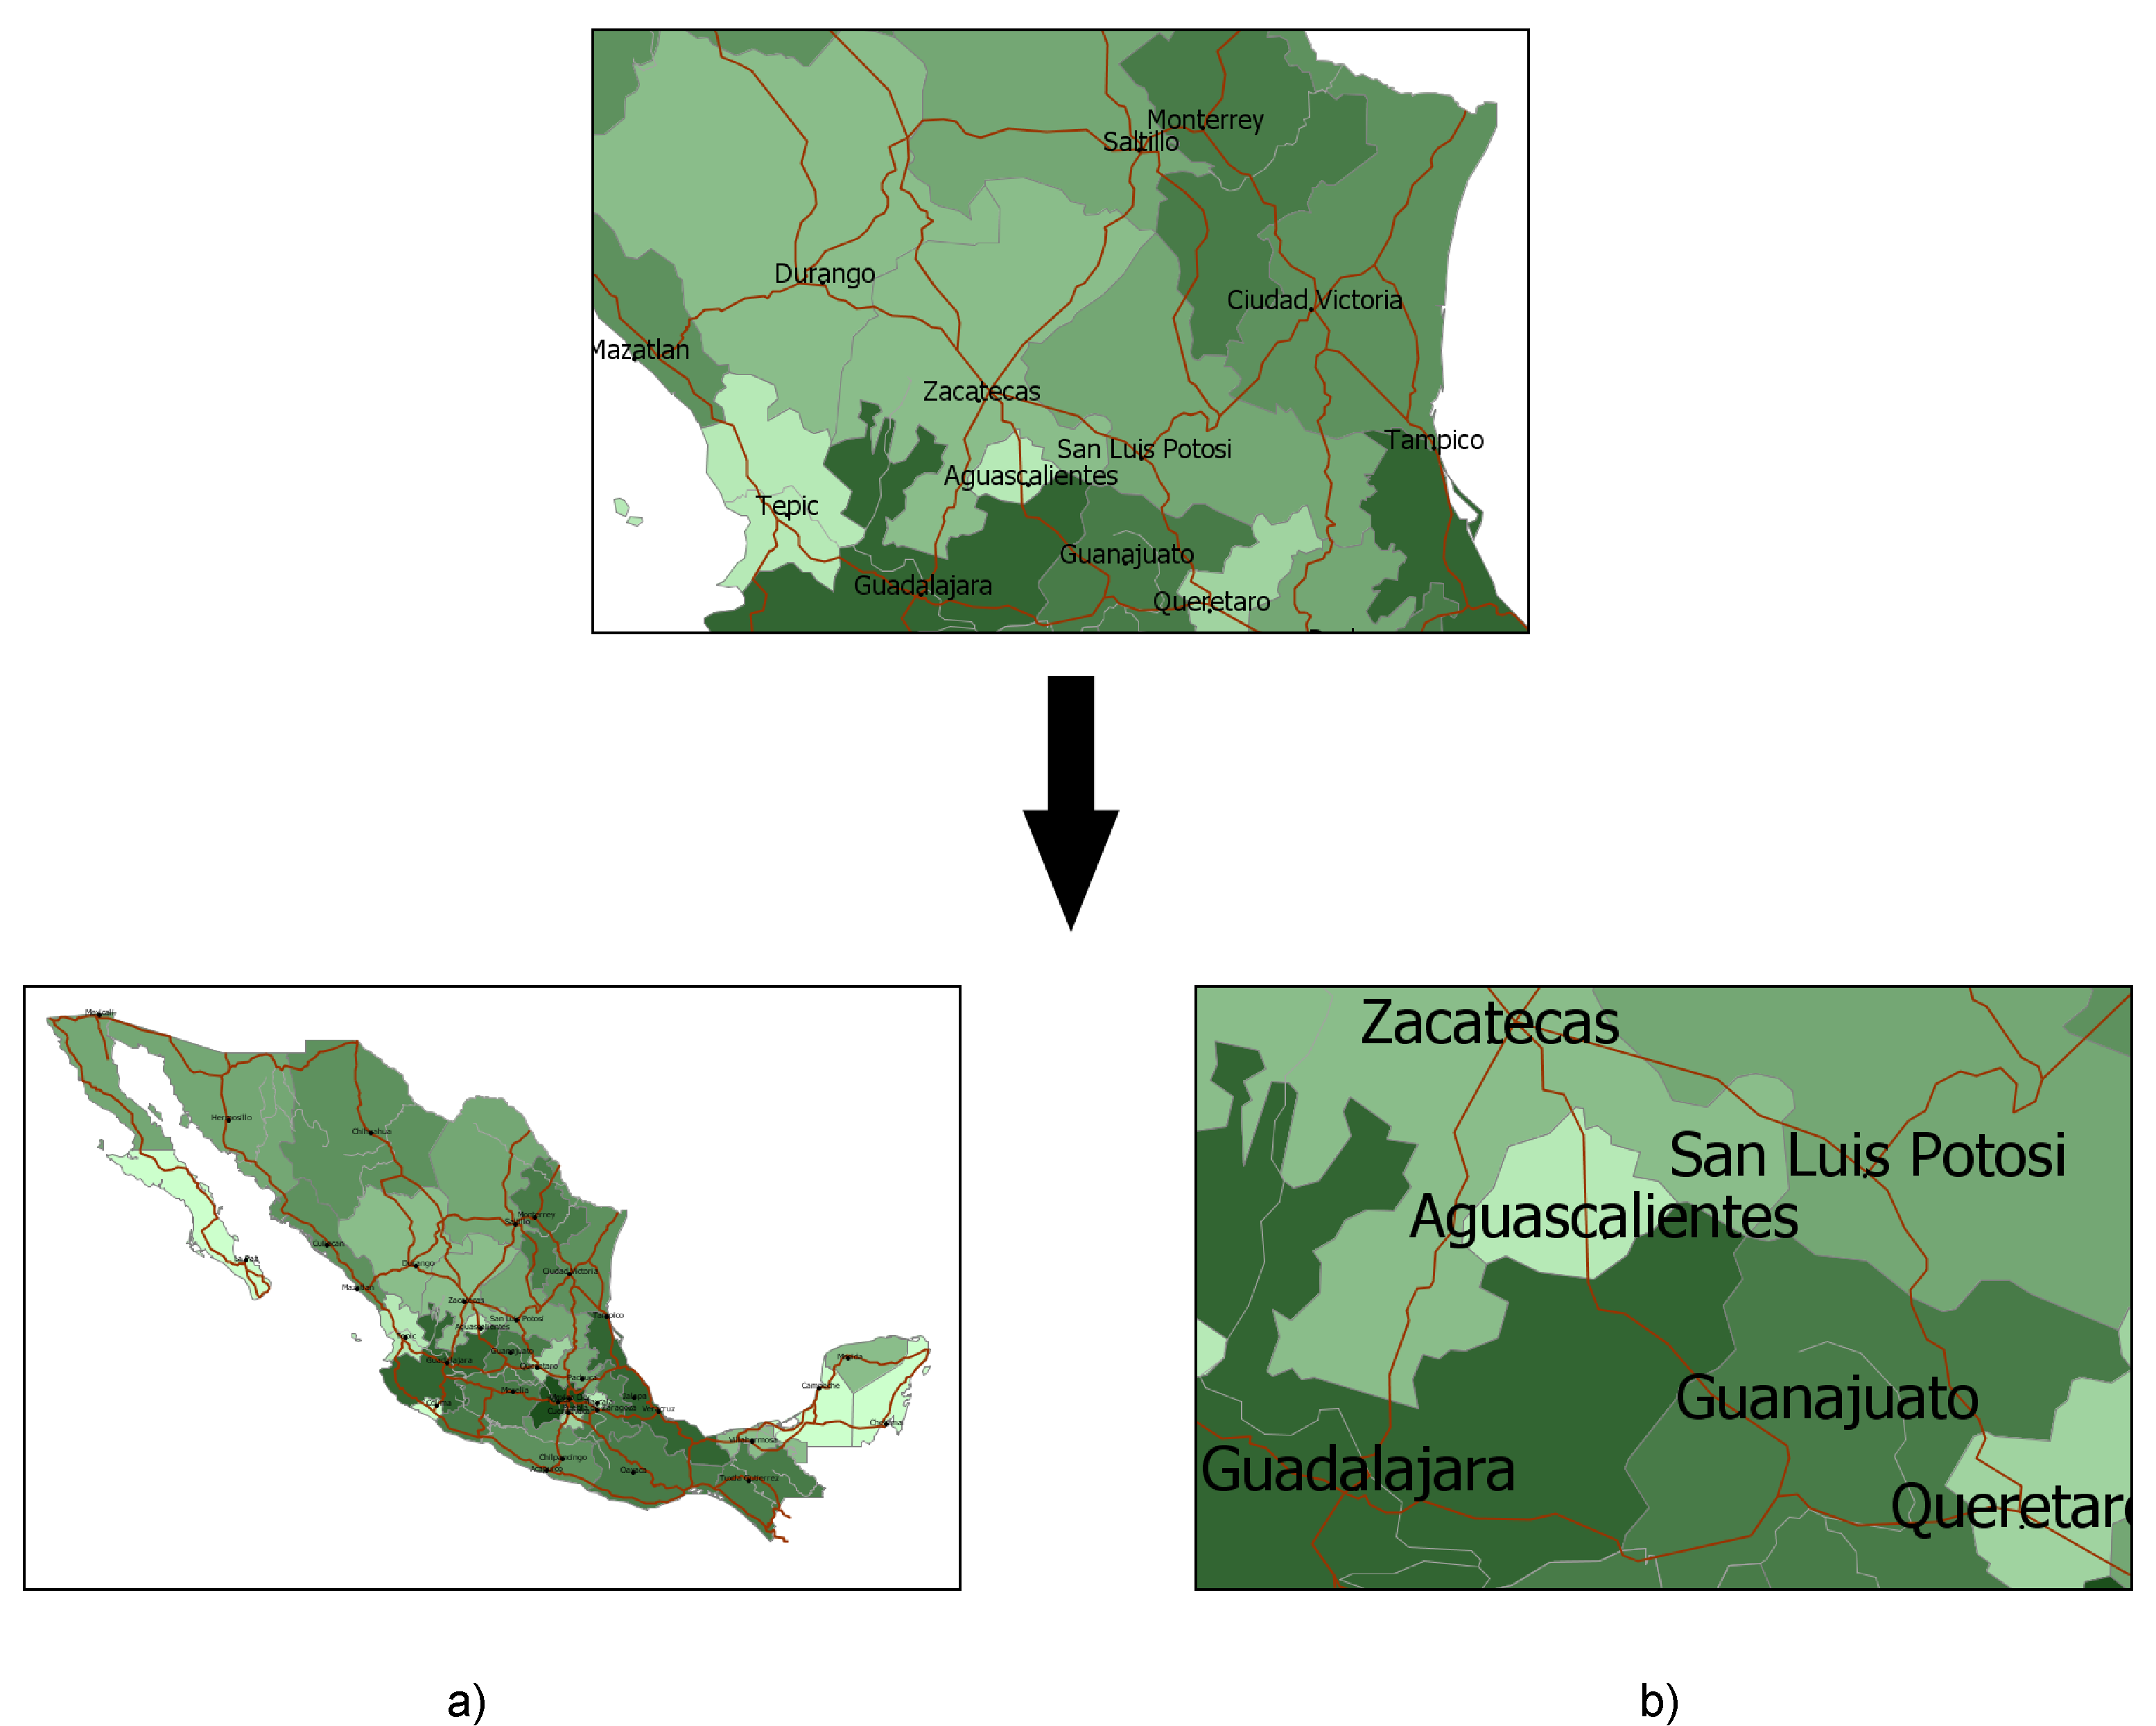
\includegraphics[width=\columnwidth]{Visualizacao/ProblemasRepresentacionSimbolos.pdf}
\caption{\small Problemas com tamanho de símbolos ao mudar a escala.}
\label{Fig:ProblemasRepresentacionSimbolos} 
\end{figure}

- Representações saturadas (Figura~\ref{Fig:RepresentacionSaturada})

\begin{figure}[!hbt]
\centering
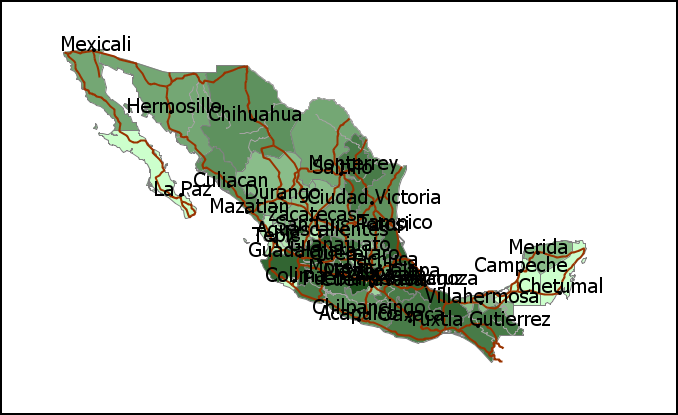
\includegraphics[width=.9\columnwidth]{Visualizacao/RepresentacionSaturada.png}
\caption{\small Representação saturada com muitos elementos.}
\label{Fig:RepresentacionSaturada} 
\end{figure}

Recomendações:

- Usar \textbf{tamanho fixo em pixels} com cautela
- Adotar abordagem \textbf{multi–escala} com diferentes camadas por escala

\pagestyle{empty}
 


\end{mainmatter}

\cleardoublepage

\end{document}


